%\chapter{det-comp}
%This chapter is split into individual files by section

%%%%%%%%%%%%%%%%%%%%%%%%%
\subsection{Overview of detector components}

\fixme{THIS SECTION IN PROGRESS}
The elements composing the detector, listed in Section~\ref{intro:detector}, include the time projection chamber (TPC), the cold electronics (CE), and the photon detection system (PDS).  Each of these elements is composed of smaller pieces, and all the components must fit together to form the whole. This section outlines how the detector is constructed by listing the components with data about their dimensions, quantities, etc., and a figure showing how they fit together.  Subsequent sections describe each component in more detail.

\begin{cdrtable}[TPC components, dimensions and quantities]{ccccccccc}{tpc-components}{TPC components, dimensions and quantities}
Major & Component  & Dimensions  & Quantity & Other characteristics &  \\ \colhline 
Element &   & Dimensions  &  &  &  \\ \toprowrule

APA &           & 5.920~m H by 2.295~m W (active) & 3 per anode plane, &  &  \\  \colhline
& &                   & 2 anode planes       &  &  \\  \colhline
       & frame & 6.06~m H, 2.3~m W, 76.2~mm thick & 1 per APA & 3 by 4 by 0.120-in SS wall tubing&  \\  \colhline
& &  &  &cross pieces 2 by 3 by 0.120-in   &  \\  \colhline
       & grid wire layer G &  full height of frame &  &  &  \\  \colhline
       & induction wire layer U &  &  &  &  \\  \colhline
       & induction wire layer V &  &  &  &  \\  \colhline
       & collection wire layer X &  &  &  &  \\  \colhline
       & mesh wire layer M &  &  &  &  \\  \colhline
& &  &  &  &  \\  \colhline
& &  &  &  &  \\  \colhline
& &  &  &  &  \\  \colhline
& &  &  &  &  \\  \colhline
& &  &  &  &  \\  \colhline
& &  &  &  &  \\  \colhline
& &  &  &  &  \\  \colhline
& &  &  &  &  \\  \colhline
& &  &  &  &  \\  \colhline
& &  &  &  &  \\  \colhline
\end{cdrtable}

In the ProtoDUNE-SP TPC, 
the six APAs are arranged into two APA planes, each consisting of three side-by-side APAs. Between them,  
a central cathode plane splits the TPC volume into two electron-drift regions, one between
each pair of facing cathode and anode planes.  A field cage (FC) must completely surround the four
open sides of the entire drift region to ensure that the electric field within is uniform and unaffected by the presence of the cryostat walls and other nearby conductive structures.

\begin{cdrfigure}[The field cages]{fc-overview}{A view of the TPC field cage}
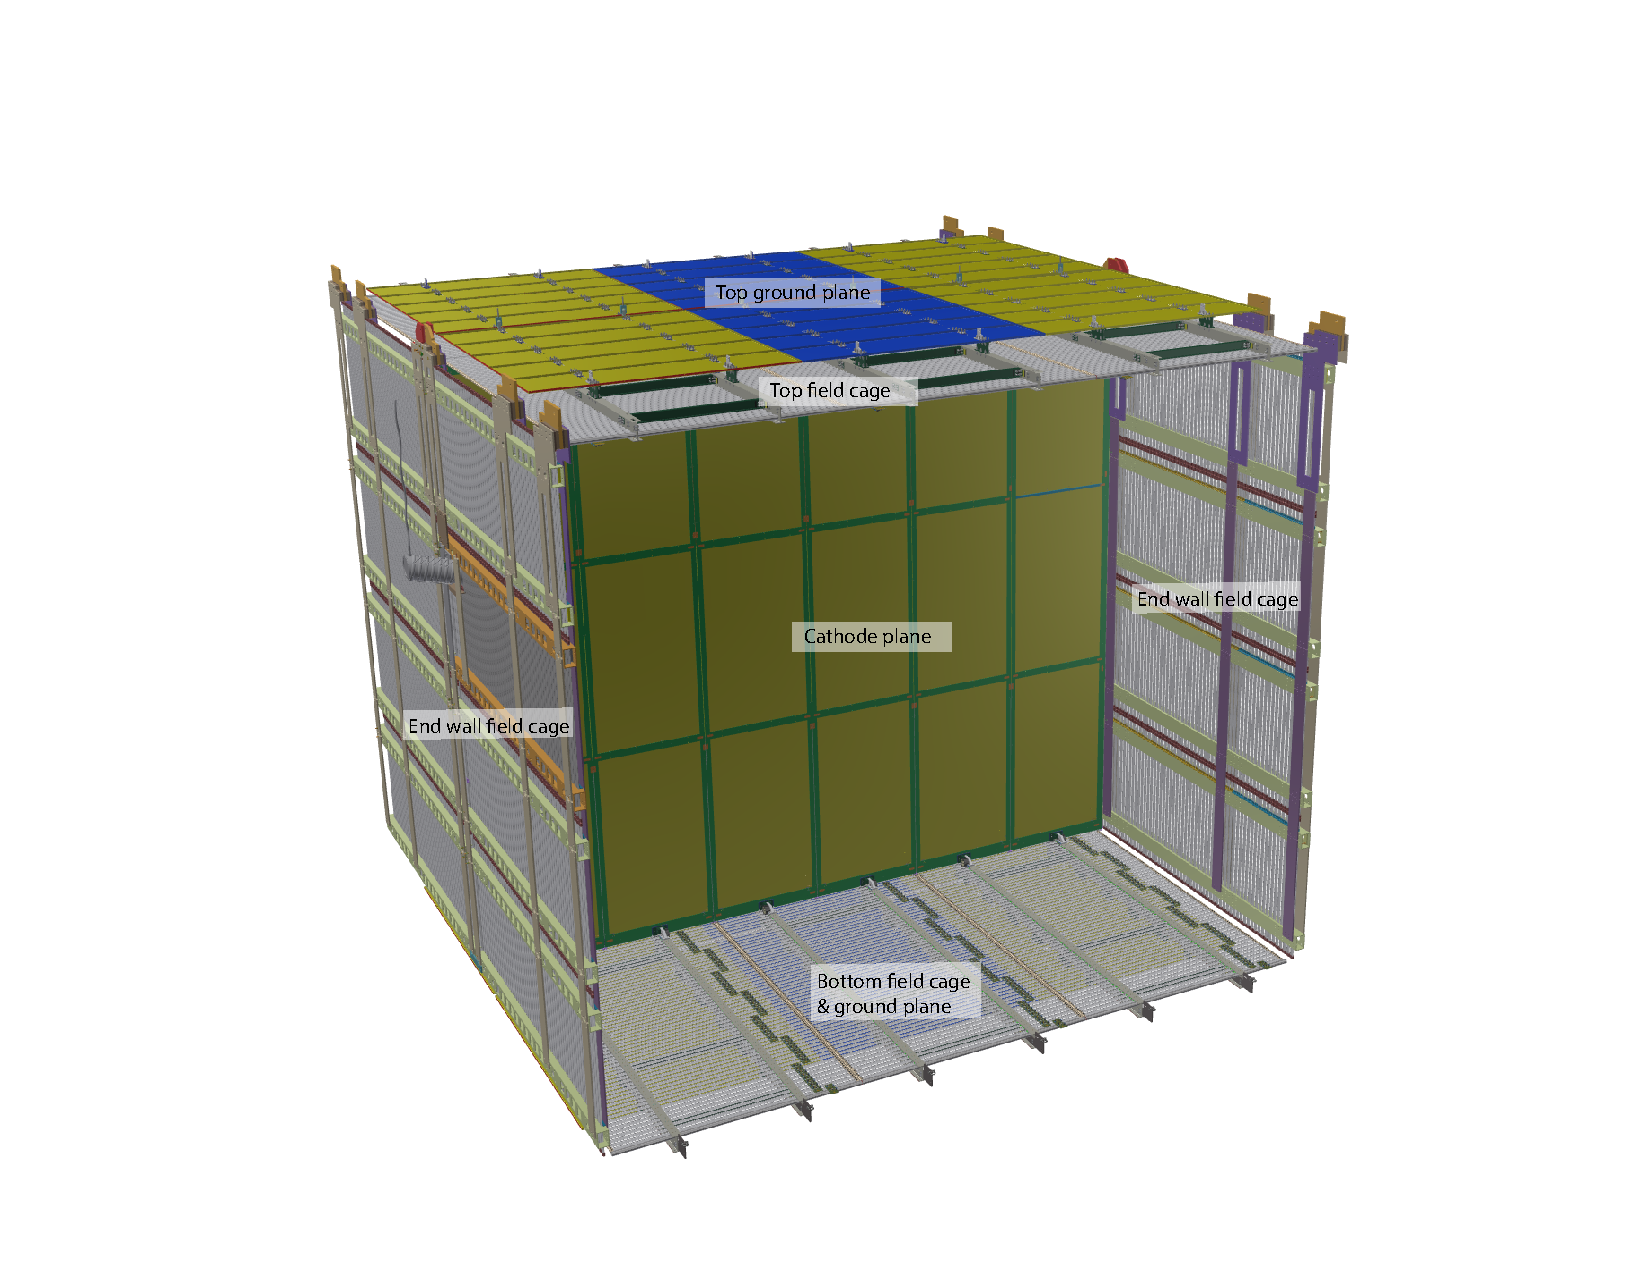
\includegraphics[width=0.6\linewidth]{tpc_fc_overview.png}
\end{cdrfigure}
\fixme{Figure~\ref{fig:fc-overview} needs a fuller, more descriptive caption}


\fixme{maybe need a bit of intro for the other components here, too}

%\chapter{det-comp}

%%%%%%%%%%%%%%%%%%%%%%%%%%%%%%%%%%%%%%%%%%%%%%
\section{Anode Plane Assemblies (APA)}

%%%%%%%%%%%%%%%%%%%%%%%%%%
\subsection{Scope and requirements}

Anode Plane Assemblies (APAs) are the detector elements utilized to sense ionization created by charged particles traversing the liquid argon volume inside the single-phase TPC.  The scope of the APAs includes:
\begin{itemize}
\item a framework of lightweight, rectangular stainless steel tubing;
\item a mesh layer attached directly to both sides of the APA frame;
\item layers of sense and shielding wires wrapped at varying angles relative to each other;
\item stacked head electronics boards, which are wire boards for anchoring the wires at the top (head) of the APA;
\item capacitive-resistive (CR) boards that link the wire boards to the CE;
\item side and foot boards along the other three edges of the APA with notches and pins to hold the wires in place;
%\item glue and solder;
\item modular boxes to hold the CE;
\item comb wire supports, mounted on cross braces distributed along the length of the APA, to prevent wire deflection; and
\item pin/slot pairs on the side edges of adjacent APAs to maintain coplanarity.
\end{itemize}

The initial physics performance requirements that drive the design of the APA are listed in Table~\ref{tab:physicsrequirements}.  These are chosen to enable high-efficiency reconstruction throughout the entire active volume of the LArTPC.  

\begin{cdrtable}[APA Physics Requirements]{lr}{physicsrequirements}{Preliminary physics requirements that motivate APA design parameters.}   
Requirement & Value  \\ \toprowrule
MIP Identification & 100$\%$ efficiency \\ \colhline
High efficiency for charge reconstruction & $>$90$\%$ for $>$100 MeV \\ \colhline
Vertex Resolution (x,y,z) & (1.5 cm, 1.5 cm, 1.5 cm)\\ \colhline
\textbf{Particle Identification} & \\ 
Muon Momentum Resolution & $<$18$\%$ for non-contained \\
            & $<$5$\%$ for contained\\ 
Muon Angular Resolution & $<$1$^{\circ}$\\            
Stopping Hadrons Energy Resolution & 1-5$\%$\\
Hadron Angular Resolution & $<$10$^{\circ}$ \\ \colhline
\textbf{Shower identification} & \\
Electron efficiency & $>$90$\%$\\
Photon mis-identification & $<$1$\%$\\
Electron Angular Resolution & $<$1$^{\circ}$ \\
Electron Energy Scale Uncertainty & $<$5$\%$\\
\end{cdrtable}

\fixme{add drawing ahead of this table showing TPC coordinate system; per Justin}

The ability to identify minimum-ionizing particles (MIPs) is a function of several detector parameters, including argon purity, drift distance, diffusion, wire pitch, and Equivalent Noise Charge (ENC).  It is required that MIPs originating anywhere inside the active volume of the detector be reconstructed with 100$\%$ efficiency.   The choice of wire pitch (i.e., $\sim$5 mm), combined with the design values of the other high-level parameters, listed in Table~\ref{tab:apaparameters},  is expected to enable  this  efficiency.

The fine wire spacing of the APA enables excellent precision in identifying the location of any vertices in an event (e.g., the primary vertex in a neutrino interaction, or gamma conversion points in a $\pi^{0}$ decay), which has a direct impact on reconstruction efficiency. It is required to reach a vertex resolution of $\sim$1.5 cm along each coordinate direction.  In practice, the resolution on the drift-coordinate ($x$) of a vertex or hit will be better than that on its location in the $y$-$z$ plane, due to the combination of drift-velocity and electronics sampling-rate uncertainties.

%%%%%%%%%%%%%%%%
\subsection{APA design overview}
\label{sec:apa-design-overview}

An APA is constructed from a framework of lightweight, rectangular stainless steel tubing, with a fine mesh covering the rectangular area within the frame, on both sides, that defines a uniform ground across the frame. Along the length of the frame and around it, over the mesh layer, layers of sense and shielding wires are strung or wrapped at varying angles relative to each other, as illustrated in  Figure~\ref{fig:tpc_apa1}. The wires are terminated on  boards that anchor them and also provide the connections to the cold electronics. The APAs are 2.3\,m wide, 6.3\,m high, and 12\,cm thick.  
The size of the APAs is chosen for fabrication purposes, compatibility with over-the-road shipping, and for eventual transport to the 4850 level at SURF and installation into the membrane cryostat of a detector module. Sufficient shock absorption and clearances are taken into account at each stage.  The dimensions are also chosen such that an integral number of electronic readout channels and boards fill in the full area of the APA. The modularity of the APAs allows them to be built and tested at off-site production facilities, decoupling their manufacturing time from the construction of the membrane cryostat. 
As mentioned above, the principal design parameters are listed in Table~\ref{tab:apaparameters}.

\begin{cdrtable}[APA Design Parameters]{lr}{apaparameters}{APA Design Parameters.}   
Parameter & Value  \\ \toprowrule
Active Height & 5.920 m\\ \colhline
Active Width & 2.295 m\\ \colhline
Wire Pitch (U,V) & 4.67 mm\\ \colhline
Wire Pitch (X,G) & 4.79 mm\\ \colhline
Wire Position Tolerance & 0.5 mm \\ \colhline
Wire Plane Spacing & 5 mm\\ \colhline
Wire Angle (w.r.t. vertical) (U,V) & 35.7$^{\circ}$\\ \colhline
Wire Angle (w.r.t. vertical) (X,G) & 0$^{\circ}$\\ \colhline
Number Wires / APA & 960 (X), 960 (G), 800 (U), 800 (V) \\ \colhline
Number Electronic Channels / APA & 2560 \\ \colhline
Wire Tension & 5.0 N \\ \colhline
Wire Material & Beryllium Copper \\ \colhline
Wire Diameter & 150 $\mu$m \\ \colhline
Wire Resistivity & 7.68 $\mu\Omega$-cm $@$ 20$^{\circ}$ C \\ \colhline
Wire Resistance/m & 4.4 $\Omega$/m $@$ 20$^{\circ}$ C \\ \colhline
Frame Planarity & 5 mm \\ \colhline
Photon Detector Slots & 10 \\
\end{cdrtable}

\fixme{Justin: The reference I always use for wire pitches is a talk by Christos from last April:
https://indico.cern.ch/event/516637/contributions/2029960/attachments/1259510/1860698/SPSC-121-protoDUNE-SP.pdf
In that talk, he has the G plane wire spacing at 4.5 mm, and the wire plane spacing at 4.8 mm, which are slightly different from the numbers in the Table here. I don’t know myself which numbers are right, but since there’s a slight discrepancy here I want to flag these up as something to be checked.}

Starting from the outermost wire layer, 
there is first a shielding (grid) plane, followed by two induction planes, and finally the collection plane. All wire layers span the entire height of the APA frame. The layout of the wire layers is illustrated in  Figure~\ref{fig:tpc_apa1}.

\begin{cdrfigure}[APA Diagram]{tpc_apa1}{Sketch of a ProtoDUNE-SP APA. This shows only portions of each of the three wire layers, U (green), V (magenta), the induction layers; and X (blue), the collection layer, to accentuate their angular relationships to the frame and to each other.  The induction layers are connected electrically across both sides of the APA.  The grid layer (G) wires (not shown), run vertically, parallel to the X layer wires;  separate sets of G and X wires are strung on the two sides of the APA.  The mesh is not shown.}
\includegraphics[width=0.8\textwidth, angle=90]{figures/tpc_apa1.png} 
\end{cdrfigure}

The angle of the induction planes in the APA ($\pm$35.7$^{\circ}$) is chosen such that each induction wire only crosses a given collection wire one time, reducing the ambiguities that the reconstruction must address.  The design angle of the induction wires, coupled with their pitch, was also chosen such that an integer multiple of electronics boards reads out one APA.

The wires of the grid (shielding) layer, G,  are not connected to the electronic readout; the wires run parallel to the long edge of the APA frame; there are separate sets of G wires on the two sides of the APA. 
 The two planes of induction wires (U and V) wrap in a helical fashion around the long edge of the APA, continuously around both sides of the APA.  The collection plane wires (X) run vertically, parallel to G.   The ordering of the layers, from the outside in, is G-U-V-X, followed by the mesh.   

The operating voltages of the APA layers are listed in Table~\ref{tab:bias}.  When operated at these voltages, the drifting ionization follows trajectories around the grid and induction wires, ultimately terminating on a collection plane wire; i.e., the grid and induction layers are completely transparent to drifting ionization, and the collection plane is completely opaque.  The grid layer is present for pulse-shaping purposes, effectively shielding the first induction plane from the drifting charge and removing the long leading edge from the signals on that layer; again, it is not connected to the electronics readout. The mesh layer serves to shield the sense planes from pickup from the Photon Detection System and from ``ghost'' tracks that would otherwise be visible when ionizing particles have a trajectory that passes through the collection plane. 

\begin{cdrtable}[Baseline bias voltages for APA wire layers]{lr}{bias}{Baseline bias voltages for APA wire layers}   
Anode Plane & Bias Voltage  \\ \toprowrule
Grid (G) & -665 V\\ \colhline
Induction (U) & -370 V\\ \colhline
Induction (V) & 0 V\\ \colhline
Collection (X) & 820 V\\ \colhline
Mesh (M) & 0 V\\
\end{cdrtable}

The wrapped style allows the APA plane to fully cover the active area of the LArTPC, minimizing the amount of dead space between the APAs that would otherwise be occupied by electronics and associated cabling.   

In the current design of the DUNE-SP far detector module, a central row of APAs is flanked by  drift-fields, requiring sensitivity on both sides. The wrapped APAs allow the induction plane wires to sense drifting ionization originating from either side of the APA.  This double-sided feature is not strictly necessary for the ProtoDUNE-SP arrangement, which has APAs located against the cryostat walls and a drift field on one side only, but it is compatible with this setup as the grid layer facing the wall effectively blocks any ionization generated outside the TPC from drifting in to the wires on that side of the APA.

The choices of wire tension and wire placement accuracy are made to ensure proper operation of the LArTPC at voltage, and to provide the precision necessary for reconstruction.  The tension of 5~N, when combined with the intermediate support combs (described in Section~\ref{subsec:apa_combs}) ensure that the wires are held taught in place with no sag.  Wire sag can impact the precision of reconstruction, as well as the transparency of the TPC.  The tension of 5~N is low enough that when the wires are cooled, which increases their tension due to thermal contraction, they will stay safely below the break load of the beryllium copper wire, as described in Section~\ref{subsec:apa_wires}.  To further mitigate wire breakage and its impact on detector performance, each wire in the APA is anchored twice on both ends, with both solder and epoxy.  %Details of this arrangement are provided in Section~\ref{subsubsec:apa_wire_wrap}. 


%%%%%%%%%%%%
\subsection{Wire properties}
\label{subsec:apa_wires}

Beryllium copper (CuBe) wire is known for its high durability and yield strength. It is composed of $\sim$98$\%$ copper, 1.9$\%$ beryllium, and a negligible amount of other elements. The APA wire has a diameter of 150$\mu$m (.006~in), and is strung in varying lengths across the APA frame. Three key properties for its usage in the APA are: low resistivity, high tensile or yield strength, and coefficient of thermal expansion suitable for use with the APA's stainless steel frame.

Tensile strength of the wire describes the wire-breaking stress (see Table~\ref{tab:wire}).  The yield strength is the stress at which the wire starts to take a permanent (inelastic) deformation, and is the important limit stress for this case, though most specifications give tensile strength.  Fortunately, for the CuBe alloys of interest, the two are fairly close to each other.  Based on the tensile strength of wire purchased from Little Falls Alloy (over 1,380~MPa or 200,000~psi), the yield strength is greater than 1,100~MPa.  Given that the stress while in use is around 280~MPa, this leaves a comfortable margin.

The coefficient of thermal expansion (CTE) describes how material expands and contracts with changes in temperature.  The CTEs of CuBe alloy and 304 stainless steel are very similar.  Integrated down to 87~K, they are 2.7e-3 for stainless and 2.9e-3 for CuBe~\cite{cryo-mat-db}.
Since the wire contracts slightly more than the frame during cool-down the wire tension increases.  If it starts at 5~N, the tension rises to about 5.5~N when everything is cool.  

The change in wire tension during cool-down could also be a concern.  In the worst case, the wire
 cools quickly to 87\,K before any significant cooling of the frame  -- a realistic case because of the differing thicknesses.  In the limiting case, with complete contraction of the wire and none in the frame, the tension would be expected to reach $\sim$11.7 N.  This is still well under the $\sim$20 N yield tension.
In practice, the cooling will be done gradually to avoid this tension spike as well as other thermal shock to the APA.

\begin{cdrtable}[CuBe wire tensile strength and CTE]{lr}{wire}{Tensile strength and coefficient of thermal expansion (CTE) of beryllium copper (CuBe) wire.}
%\multicolumn{2}{c}{Properties of beryllium copper wire} \\ 
Parameter & Value \\ \toprowrule
Tensile Strength (from property sheets) (psi) & 208,274 \\ \colhline
Tensile Strength (from actual wire) (psi) & 212,530 \\ \colhline
CTE of CuBe, integrated to 87 K (m/m) & 2.9e-3 \\ \colhline
CTE of 304 stainless steel, integrated to 87 K (m/m) & 2.7e-3 \\
\end{cdrtable}


%%%%%%%%%%%%
\subsection{APA frame and mesh}
\label{subsec:apa_frame}

%\paragraph{Dimensions}

The stainless steel frame of the APA (Figure~\ref{fig:tpc_apa_framedrawing}) is 6.06~m long, not counting electronics and mounting hardware, and 2.30~m wide.  It is 76.2~mm thick, made from imperial size 3-in $\times$ 4-in $\times$ 0.120-in wall rectangular tubing.  The cross pieces have a cross-sectional area of 2\,in $\times$ 3\,in, and are connected to edge pieces using joints, as in Figure~\ref{fig:tpc_apa_boltedjointdrawing}.  It is mounted in the cryostat with its long axis vertical; multiple APAs are mounted edge-to-edge to form a continuous plane. An electron deflection technique is used to ensure that electrons drawn towards a joint between two APAs will be deflected to one or the other, and not lost.

\fixme{Justin: describe electron deflection technique }

\begin{cdrfigure}[APA dimensions]{tpc_apa_framedrawing}{An APA showing overall dimensions and main components. }
\includegraphics[width=0.9\textwidth]{figures/tpc_apa_framedrawing.png} 
\end{cdrfigure}
\fixme{COMMENT from Justin: it would be good if the dimensions of the upper figure had the same precision as the numbers in the text, i.e. 6.06 m and 2.30 m. (Anne agrees, but we're not updating figures right now.)}

\begin{cdrfigure}[APA Bolted Joint Drawing]{tpc_apa_boltedjointdrawing}{A model of the bolted joint.  The holes on the top of the tube are for access to tighten the screws.  The heads actually tighten against the lower hole, inside the tube.}
\includegraphics[width=0.4\textwidth]{figures/tpc_apa_boltedjointdrawing.png} 
\end{cdrfigure}

A fine mesh screen is glued directly to the steel frame surface, over the frame on both sides.  It creates a uniform ground layer beneath the wire planes.  

The mesh is clamped around the perimeter of the opening and then pulled tight (by opening and closing clamps as needed during the process).  When the mesh is taut, a 25-mm-wide strip is masked off around the opening and glue is applied through the mesh to attach it to the steel.  Although measurements have shown that this gives good electrical contact between the mesh and the frame, a deliberate electrical connection is also made.  Figure~\ref{fig:tpc_apa_fullsizemeshdrawing} depicts the mesh application setup for a full-size ProtoDUNE-SP APA.

\begin{cdrfigure}[APA Full-Size Mesh Drawing]{tpc_apa_fullsizemeshdrawing}{The mesh clamping jig for the full size APA. }
\includegraphics[width=0.8\textwidth]{figures/tpc_apa_fullsizemeshdrawing.png} 
\end{cdrfigure}

\fixme{COMMENT from Justin: this jig is currently being redesigned. If the design changes significantly, we should remember to update this picture.}


%%%%%%%%%%%%%%%%%%%%%%%%
\subsection{Anchoring elements and wire boards}
\label{subsubsec:apa_wire_anchor}


%%%%%%%%%%%%
\subsubsection{Head electronics boards}

At the head end of the APA, stacks of electronics boards (referred to as ``wire boards'') are arrayed to anchor the wires.  They also provide the connection between the wires and the %data acquisition electronics -- usually called the 
cold electronics.

All APA wires are terminated on the wire boards, which are stacked along the electronics end of the APA frame; see Figure~\ref{fig:tpc_apa_boardstack}. 
Attachment of the wire boards begins with the X plane (innermost). After the X-plane wires are strung top to bottom along each side of the APA frame, they are soldered and epoxied to their wire boards and trimmed. The remaining wire board layers are attached as each layer is wound.  The main CR boards (capacitive-resistive), which provide DC bias and AC coupling to the wires, are attached to the bottom of the wire board stack. They are described in Section~\ref{sec:crboards}.

\begin{cdrfigure}[APA Board Stack]{tpc_apa_boardstack}{Left: View of the APA wire board stack, as seen from the top/side. The wire board layers can be seen at the bottom-left of the illustration, X on the bottom (it doesn't go all the way back, but extends farther forward and has the main CR board attached), followed by U, V, then G (which doesn't go all the way forward, and has its own CR board attached).  Right: the same stack viewed from below.  }
\includegraphics[width=0.45\textwidth]{figures/tpc_apa_boardstack_top.png}
\includegraphics[width=0.45\textwidth]{figures/tpc_apa_boardstack_bottom.png}
\end{cdrfigure}

\fixme{figure \ref{fig:tpc_apa_boardstack} needs labeling}

The outermost G-plane wire boards connect adjacent groups of four wires together, and bias each group through an R-C filter whose components are placed on special CR boards  %The filter components are located on daughter boards 
that are attached after the wire plane is strung. The X, U and V layers of wires are connected to the CE (housed in boxes mounted on the APA) either directly or through DC-blocking capacitors. The X and U planes have wires individually biased through 50-M$\Omega$ resistors. Electronic components for the X- and U-plane wires are located on a common CR board. 

Mill-Max pins and sockets provide electrical connections between circuit boards within a stack. They are pressed into the circuit boards and are not repairable if damaged. To minimize the possibility of damaged pins, the boards are designed so that the first wire board attached to the frame has only sockets. All boards attached subsequently contain pins that plug into previously mounted boards. This process eliminates exposure of any pins to possible damage during winding, soldering, or trimming processes.

Ten stacks of wire boards are installed across the width of each side along the head of the APA.  The X-layer board in each stack has room for 48 wires, the V layer has 40 wires, the U layer 40 wires and the G layer 48 wires.  Each board stack, therefore, has 176 wires but only 128 signal channels since the G wires are not read out.  
With a total of 20 stacks per APA, this results in 2,560 signal channels per APA and a total of \SI{3520} wires starting at the top of the APA and ending at the bottom.  There is a total of $\sim$23.4 km of wire on the two surfaces of each APA.  Many of the capacitors and resistors that in principle could be on these wire boards are instead
placed on the attached CR boards to improve their accessibility in case of component failure.   Figure~\ref{fig:tpc_apa_electronics_connectiondiagram} depicts the connections between the different elements of the APA electrical circuit. \fixme{this figure could use some labelling}

At the head end of the APA, the wire-plane spacing is set by the thickness of these wire boards.  The first layer's wires solder to the surface of the first board, the second layer's wires to the surface of the second board, and so on.  For installation, temporary toothed-edge boards beyond these wire boards align and hold the wires until they are soldered to pads on the wire boards.  After soldering, the extra wire is snipped off. 

\begin{cdrfigure}[APA wire board connection to electronics]{tpc_apa_electronics_connectiondiagram}{Diagram of the connection between the APA wires, viewed from the APA edge. The set of wire boards within a stack can be seen on both sides of the APA, with the CR board extending further to the right, providing a connection to the cold electronics, which are housed in the boxes at the far right of the figure}.
\includegraphics[width=0.7\textwidth]{figures/tpc_apa_electronics_connectiondiagram.png}
\end{cdrfigure}

%%%%%%%%%%%%
\subsubsection{CR boards}
\label{sec:crboards}

The CR boards carry a bias resistor and a DC-blocking capacitor for each wire in the X and U planes. These boards are attached to the board stacks after fabrication of all wire planes.  Electrical connections to the board stack are made though Mill-Max pins that plug into the wire boards. Connections from the CR boards to the CE are made through a pair of 96-pin Samtec connectors.

Surface-mount bias resistors on the CR boards have resistance of 50\,M$\Omega$ are constructed with a thick film on a ceramic substrate. Rated for 2.0-kV operation, the resistors measure 0.12 $\times$ 0.24 inches. Other ratings include operation from $-$55 to +155 C, 5\% tolerance, and a 100-ppm/C temperature coefficient.
Performance of these resistors at LAr temperature is verified through additional bench testing.

The selected DC-blocking capacitors have capacitance of 3.9\,nF and are rated for 2.0-kV operation. Measuring 0.22 $\times$ 0.25\,inches across and 0.10\,inches high, the capacitors feature flexible terminals to comply with PC board expansion and contraction. They are designed to withstand 1,000 thermal cycles  
between the extremes of the operating temperature range. Tolerance is also 5\%.

\fixme{Eric has question mark on the temp range}

In addition to the bias and DC-blocking capacitors for all X- and V-plane wires, the CR board includes two R-C filters for the bias voltages. The resistors are of the same type used for wire biasing except with a resistance of 2\,M$\Omega$. Capacitors are 47\,nF at 2\,kV. Very few choices exist for surface-mount capacitors of this type, and they are exceptionally large. %Currently the plan is to use 
Polyester or Polypropylene film capacitors that are known to perform well at cryogenic temperatures are used.


%%%%%%%%%%%%
\subsubsection{Side and foot boards}

The boards along the sides and foot of the APA have notches, pins and other location features to hold the wires in the correct position as they wrap around the edge from one side of the APA to the other.

G10 circuit board material is ideal for these side and foot boards due to its physical properties alone, but it has an additional advantage: a number of hole or slot features in the edge boards provide access to the underlying frame.  In order that these openings are not covered by wires, the sections of wire that would go over the openings are replaced by traces on the boards.  After the wires are wrapped, the wires over the opening are soldered to pads at the ends of the traces, and the section of wire between the pads is snipped out (Figure~\ref{fig:tpc_apa_sideboardmodel}).  These traces are easily and economically added to the boards by the many commercial fabricators who make circuit boards. 

\begin{cdrfigure}[APA Side Board Model]{tpc_apa_sideboardmodel}{Model of board with wires showing how traces connect wires around openings in the side boards.  The wires are wound straight over the openings, then soldered to pads at the ends of the traces.  After soldering the sections between the pads are trimmed away.}
\includegraphics[width=0.9\textwidth]{figures/tpc_apa_sideboardmodel.png} 
\end{cdrfigure}


\begin{cdrfigure}[APA Side Board Photo]{tpc_apa_sideboardphoto}{Boards with injection molded tooth strips glued on.  The left shows an end board with teeth for fixing the position of the longitudinal wires.  The teeth there form small notches. The right is a side board for fixing the position of the angled wires where the wires are angled around a pin.}
\includegraphics[width=0.7\textwidth]{figures/tpc_apa_sideboardphoto.png} 
\end{cdrfigure}

The placement of the angled wires are fixed by pins 
as shown in the right-hand picture of Figure~\ref{fig:tpc_apa_sideboardphoto}.  The wires make a partial wrap around the pin as they change direction from the face of the APA to the edge.  The X- and G-plane wires are not pulled to the side so they cannot be pulled against a pin.  Their positions are fixed %located 
by teeth with slots, as shown in the left-hand picture in Figure~\ref{fig:tpc_apa_sideboardphoto}. 
	
The polymer used for the strips is Vectra e130i (a trade name for 30$\%$ glass filled liquid crystal polymer or LCP). It retains its strength at cryogenic temperature and has a CTE similar enough to G10 that differential expansion/contraction is not a problem.

%%%%%%%%%%%%
\subsubsection{Glue and solder}
The ends of the wires are soldered to pads on the edges of the wire boards.  Solder provides both an electrical connection and a physical anchor to the wires.  As an additional physical anchor, roughly 10~mm of the wires are glued near the solder pads.  For example, in Figure~\ref{fig:tpc_apa_sideboardphoto}, in addition to soldering the wires on the pads shown in the left-hand photograph, an epoxy bead is applied on the wires in the area between the solder pads and the injection-molded tooth strips.

Gray epoxy 2216 by 3M is used for the glue.  It is strong, widely used (therefore much data is available), and it retains good properties at cryogenic temperatures.  A 62$\%$ tin, 36$\%$ lead and 2$\%$ silver solder was chosen.  A eutectic mix (63/37) is the best of the straight tin/lead solders but the 2$\%$ added silver gives better creep resistance.

%%%%%%%%%%%%
\subsubsection{Comb wire supports on inner frame members}
\label{subsec:apa_combs}

%\paragraph{Purpose}

Some wire segments are quite long; for instance, the X- and G-plane wires 
extend from one end of the APA to the other without going around a side -- a length of 6\,m.  Even the diagonal wires across the middle of the APA are 3.9\,m long.  To prevent deflection from gravity, electrostatic forces, or liquid drag from moving argon, the wires are supported at regular locations along the length of the APA.  This is done with \textit{combs} mounted on each of the four cross braces that are  %evenly 
regularly spaced along the length of the APA.  This keeps the longest unsupported wire length under 1.6\,m.

The nominal wire tension is 5\,N but even the 1.6-m-long wires could fall to 3\,N of tension before the wire, held horizontally, would deviate 150\,microns -- one wire diameter.  During operation the wires are either vertical or 35.7$^{\circ}$ from vertical, so the actual deviation would be less.

%\paragraph{Geometry}

The combs are made from 0.5-mm-thick G10 with slots cut into it.  The comb for the lowest layer is glued to a base strip that is glued to the frame.  After each layer is wound, another comb strip is glued to the tips of the teeth of the previous one to position the wires in the next layer.  Each successive comb holds the previous layer of wires in the bottom of its slots (Figure~\ref{fig:tpc_apa_supportcombmodel}).

\begin{cdrfigure}[APA Support Comb Model]{tpc_apa_supportcombmodel}{A model of the combs showing how they stack.  After winding a layer, the comb for the next layer is put in place.  Each comb holds the wires from the previous layer in its slots.}
\includegraphics[width=0.7\textwidth]{figures/tpc_apa_supportcombmodel.png} 
\end{cdrfigure}

Periodic holes along the length of the strip allow the use of pins to accurately position each successive strip with respect to the previous one.  A series of jigs is used to create and install these combs.  One jig aligns the first strip to the base strip during gluing.  Another jig locates this assembly on the frame as it is glued in place. A third jig locates each successive comb using these holes (labeled registration holes in Figure~\ref{fig:tpc_apa_supportcombmodel}).

The wire openings in the comb stack are small enough that the wires are accurately positioned at the combs, and therefore the gluing of wires into the combs is not required.

%%%%%%%%%%%%
\subsection{Cabling}
\fixme{Justin: Something that’s being discussed a lot at the moment is how the APAs will be cabled up. Is there a section somewhere else in the TDR that covers cabling? 
(It’s fine for it to be in a different section, but I think it’s important that it’s covered in the TDR.) (Anne says I don't find this topic covered. Not sure we need a full subsection or not, but am putting this here as a placeholder) }

%%%%%%%%%%%%
\subsection{Interconnection features}

%%%%%%%%%%%%
\subsubsection{CE boxes}

Pins extending outward from the CR boards provide connections from the APA to the modularly designed CE, and the CE modules are housed in small boxes that provide shielding.
The CE boxes are illustrated in Figure~\ref{fig:tpc_apa_electronicsmountingdiagram}. 
%The design being developed for attaching the CE to the APAs consists of small boxes, 
Each board stack has one CE box installed near it that holds the CE module for the stack.  

Putting the electronics in small boxes simplifies installation and replacement, and also helps with the dissipation 
\fixme{getting rid of}
of argon gas generated by the warm electronic components.  The CE modules are mounted in such a way that any of them can be removed from a single side of the APA after APA installation.

\begin{cdrfigure}[Solid model of modular CE boxes]{tpc_apa_electronicsmountingdiagram}{Solid model of %revised, 
modular CE boxes.}
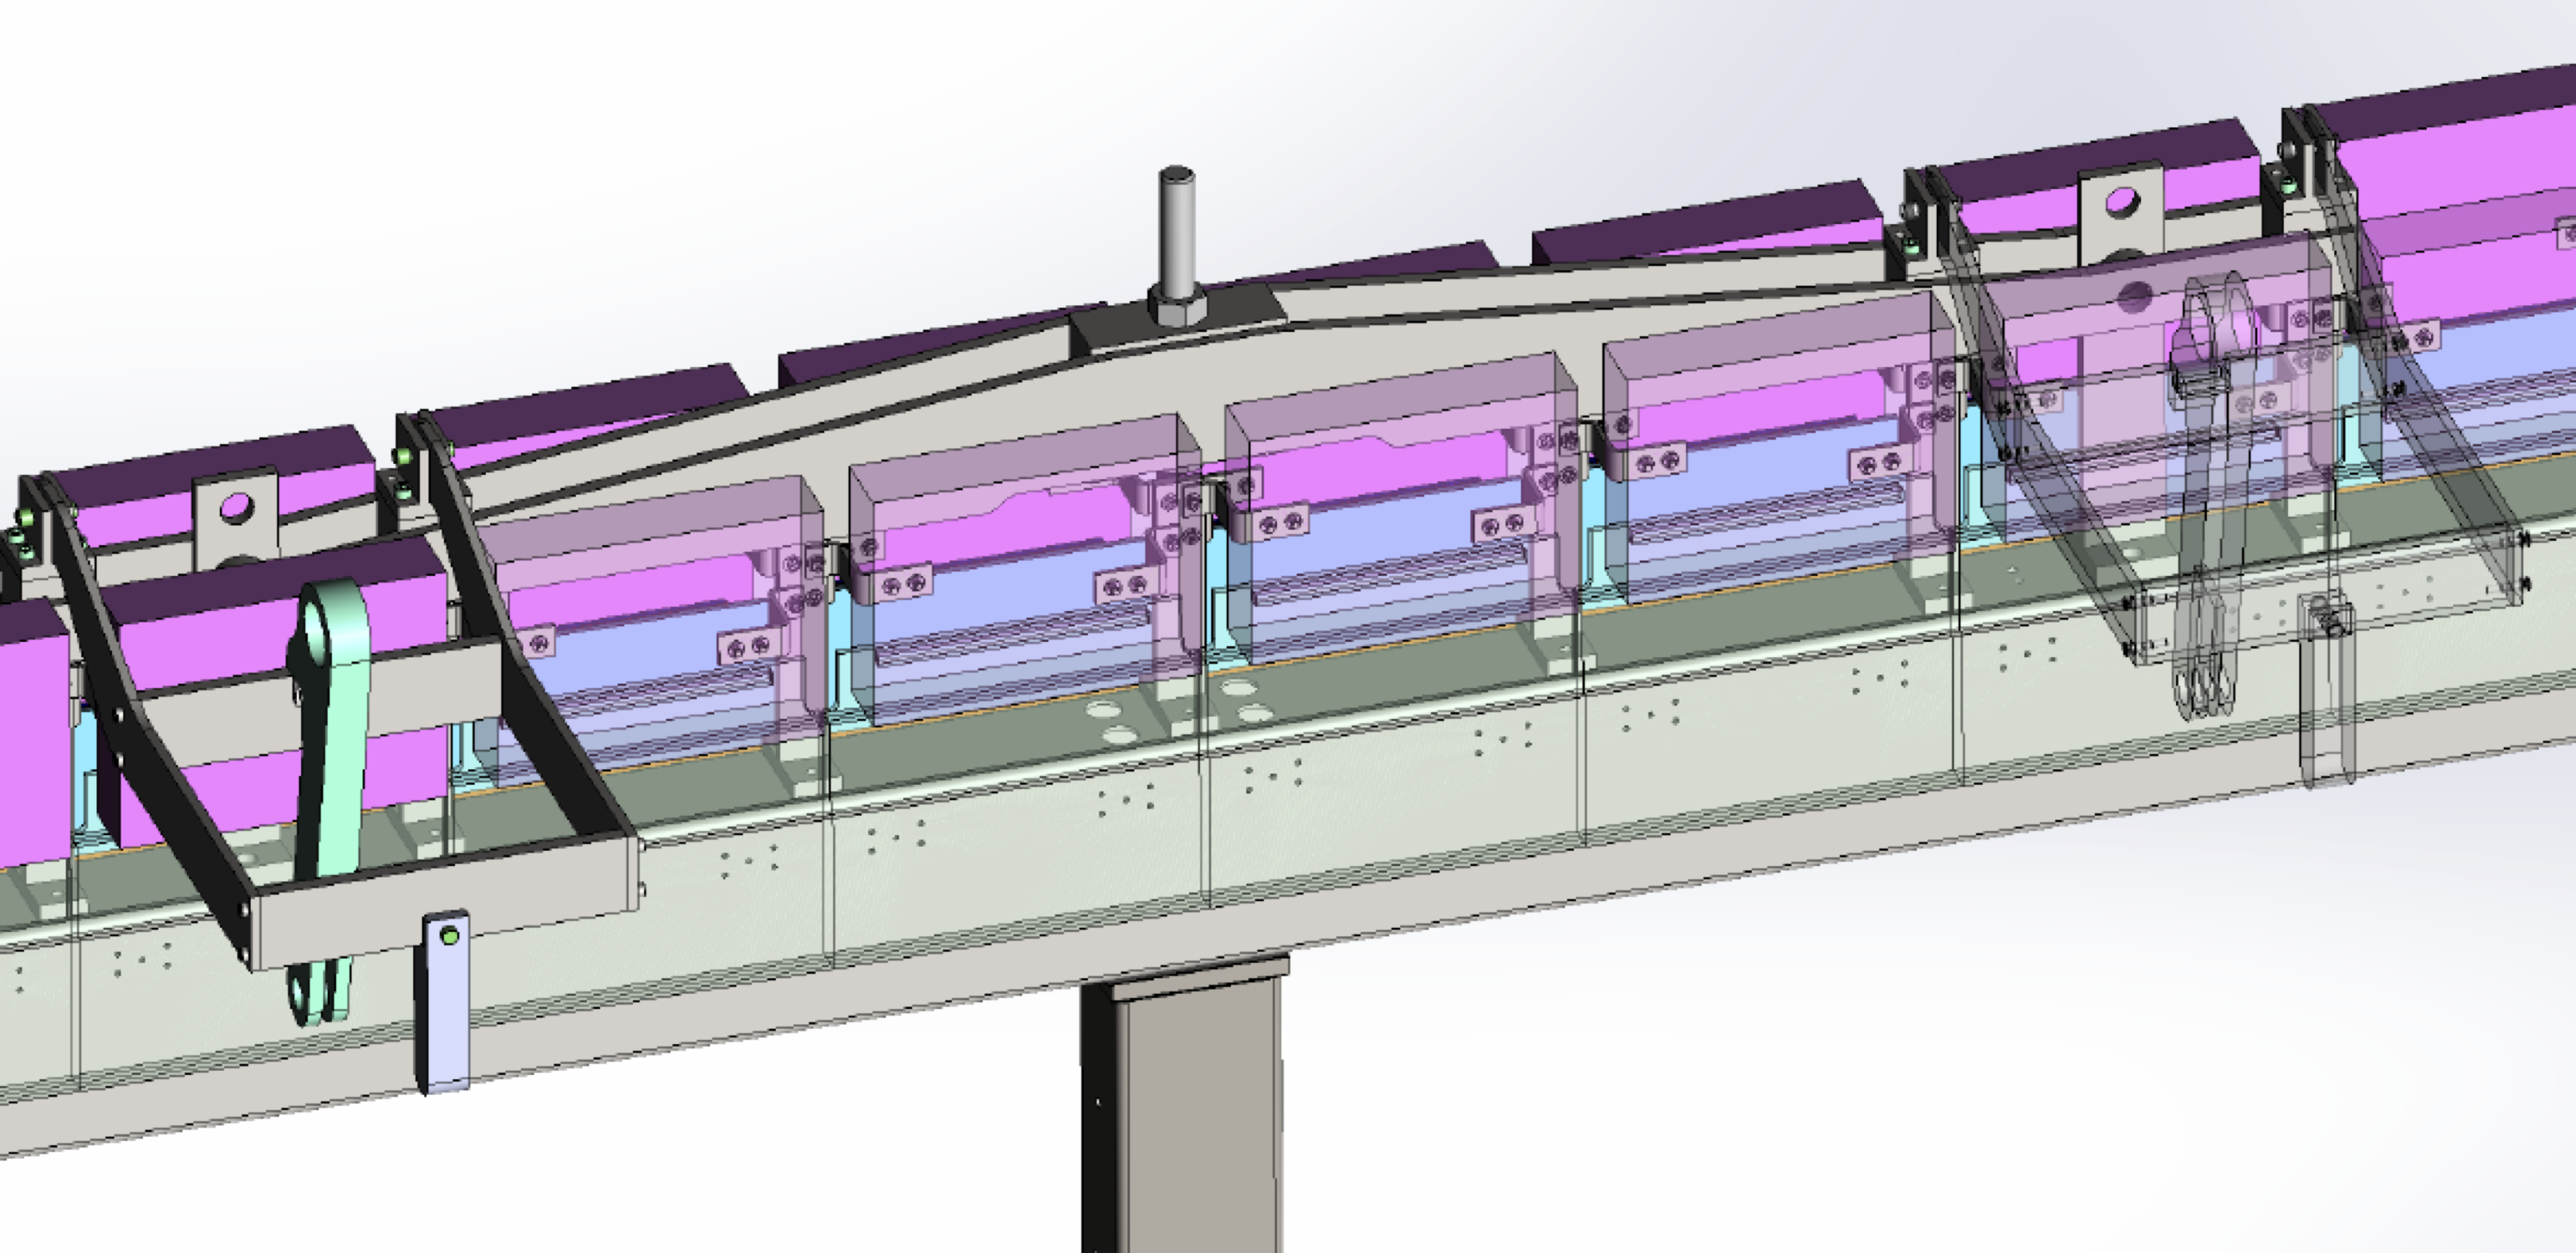
\includegraphics[width=0.9\textwidth]{figures/tpc_apa_electronicsmountingdiagram.png} 
\end{cdrfigure}

%%%%%%%%%%%%
\subsubsection{Adjacent APAs}

A constraint is needed between adjacent APAs to keep them co-planar.  It is also important that this constraint not apply a vertical load to adjacent APAs.  The constraint takes the form of 
 a pair of protruding pins on one edge of the APA (one high and one low) and a pair of matching slots %on the other edge 
on the edge of the adjacent APA
to engage the pins (Figure~\ref{fig:tpc_apa_pinslotdrawing}). The pins have steel cores for strength.

\begin{cdrfigure}[APA Interconnect Drawing]{tpc_apa_pinslotdrawing}{The pin/slot constraint.  The pin screws into an insert in the outside frame member of one APA and engages a slot in the outside frame member of the adjacent APA.}
\includegraphics[width=0.9\textwidth]{figures/tpc_apa_pinslotdrawing.png} 
\end{cdrfigure}

Electronics noise concerns have made it desirable to isolate APAs from each other.  Therefore, the alignment pins have G10 sleeves covering their steel cores at places where they come into contact with the frame of the adjacent APA.



%\chapter{det-comp}


%%%%%%%%%%%%%%%%%%%%%%%%%%%%%%%%%%%%%%%%%%%%%%
%\section{Anode Plane Assemblies}

%%%%%%%%%%%%%%%%%%%%%%%%%%%%%%%%%%%%%%%%%%%%%%
\section{Cathode Plane Assembly (CPA)}
\label{sec:cpa}

%\subsection{Scope, requirements and design considerations}
\subsection{Scope and requirements}

The cathode plane, also called the cathode plane assembly, or CPA, is located in the middle of the TPC, dividing the detector into two equal-distance drift volumes. The cathode plane's 7\,m $\times$ 6\,m area is made up of six \textit{CPA columns}, each of which is constructed of three vertically stacked \textit{CPA modules}. The CPA therefore consists of 18 CPA modules. 

The scope of the CPA includes:

\begin{itemize}
\item 18 CPA modules, each with a frame and resistive cathode panel, 
\item HV bus connecting the CPA columns and modules, and
\item HV cup for receiving input from the power supply.
\end{itemize}


%%%%%%%%%%%%%%%%%%%%%%%%%
%\subsubsection{Requirements}
The CPA plane is required to:
\begin{itemize}
\item provide equipotential surfaces at $-$180kV nominal bias voltage,
\item maintain a flatness better than 1~cm when submerged in the liquid argon,
\item be constructed of materials with comparable CTEs to that of stainless steel, 
\item limit the electric field exposed to LAr to under 30~kV/cm 
\item prevent damage to the TPC, including its readout electronics, in case of a HV discharge anywhere on the cathode,
\item provide constant bias voltage and current to all attached field cage (FC) resistor divider chains,
\item support the full weight of the four connected top/bottom FC modules plus a person on the bottom FC during installation,
\item accommodate cryostat roof movement between warm and LAr-filled states,
\item be constructed in a modular form that can be easily installed in the cryostat,
\item accommodate Photon Detection System (PDS) calibration features, and
\item avoid any trapped volume of LAr.
\end{itemize}

%%%%%%%%%%%%%%%%%%%%%%%%%
\subsection{Design considerations}


For the future DUNE-SP far detector, the cathode planes are planned to be 12\,m tall by nearly 60\,m long.  When biased to the nominal voltage of $-$180\,kV, each of these cathode planes stores more than 100\,J of energy. If this energy were to be released  suddenly and completely in a high-voltage discharge event, it could greatly affect the integrity of the detector elements, including the sensitive front-end electronics.  
Study has shown~\cite{cathode-hv-1320} that a cathode plane made of interconnected metallic electrodes would present significant risk to the front-end ASICs based on the potential charge injection through the capacitive coupling between the cathode and the anode wires originating from such an event.  

To address this issue in ProtoDUNE, the entire cathode plane is made out of highly resistive material such that it has a very long discharge time constant.  In the event of HV breakdown at a given location on the cathode plane, the sudden change in voltage is restricted to  a relatively localized area on the CPA module in question.  The rest of the CPA maintains its original bias voltage, and gradually discharges to ground through the large resistivity of the cathode material.  This greatly reduces the instantaneous charge injection to the front-end electronics.


%%%%%%%%%%%%%%%%%%%%%%%%%
\subsection{CPA design}

%%%%%%%%%%%%%%%%%%%%%%%%%
\subsubsection{CPA modules}

%The cathode plane design has evolved through several iterations over the years.  The design chosen for the ProtoDUNE-SP TPC is an array of moderately sized modules constructed from strong FR4 (the fire-retardant version of G10) frames holding thin FR4 sheets laminated with a commercial resistive Kapton film on both sides.   Compared with the size of an APA, the CPA modules are 1/2 in width (1.16\,m) and 1/3 in height (2\,m).   Each module has four FR4 bars holding a 3mm thick FR4 sheet with resistive coating.  The thickness of the FR4 bars is 6cm.  The surfaces of the bars facing the APAs are covered by another set of resistive FR4 strip with a different bias voltage such that these FR4 bars do not cause any distortion in the drift field beyond the resistive surfaces.

The cathode plane design chosen for the ProtoDUNE-SP TPC is an array of 18 moderately sized modules constructed from strong 6-cm-thick FR4 (the fire-retardant version of G10) frames. The frames hold 3-mm-thick FR4 panels laminated on both sides with a commercial resistive Kapton film.   Each CPA module is 1.16\,m wide and 2\,m high, and they stack to form six CPA columns of height 6\,m.  The six-column-wide CPA has the same dimensions as each of the two APA planes, with a width of about 7\,m.

 The surface of the frame facing the APAs is covered by a set of resistive FR4 strips with a different bias voltage, set such that 
 the frame itself causes no distortion in the drift field beyond the resistive surfaces.

Each CPA column is suspended under the cathode support rail by a single insulating FR4 bar.  On the top and bottom edges of a CPA, two hinges support the partial weight of the top and bottom field cage modules.   Adjacent CPAs are aligned through pin-and-slot connections to maintain co-planarity while allowing minor relative vertical shifts due to cryostat roof movement.

The electrical connectivity of the resistive panels within a CPA column is maintained by several tabs through the edge frames.  There is no direct electrical connection across the CPA columns. 
Instead, the voltage is passed from one column to another through embedded cables in the CPA panels referred to collectively as the HV bus.  Redundant connections in the HV bus between CPA columns are used to ensure reliability.  
The HV bus also provides a low-resistance path for the voltage needed to operate the FC resistive divider chains.
The required connections to the FC modules are made at the edges of the cathode plane. 
Along the perimeter of the CPA, the HV bus cables are hidden between the field-shaping strip overhang and the main cathode resistive sheet.  The cables must be capable of withstanding the full cathode bias voltage to prevent direct arcing to (and as a result, the recharging of) a CPA panel that discharges to ground. 

The outer edges of the cathode plane facing the cryostat wall are populated with the same metal profiles, with insulating polyethylene caps, as used in the field cage.  This eliminates the need for a special design of the most crucial regions of the cathode plane: the edges of the CPA now look just like a continuation of the FC.  Since these profiles are the only objects facing grounded surfaces, they are the most likely candidates to have HV discharges to ground.   To limit peak current flow, these edge profiles are resistively connected to the field shaping strips.

%to the main cathode panels through
%their laminated resistive surfaces.  

The resistive surface concept is illustrated in Figure~\ref{fig:cpa-concept}.

\begin{cdrfigure}[Resistive surface CPA concept]{cpa-concept}{The resistive surface CPA concept showing  
 a 3D model of a corner of the cathode with major components.} 
\includegraphics[width=\linewidth]{tpc_cpa_concept_leftonly}
\end{cdrfigure}


The CPA is connected to the HV feedthrough through a receptacle, called the \textit{HV cup}, at the back end of the cryostat (with respect to the beam entrance) and biased at $-$180\,kV.   It provides this voltage and the required current to all the FC modules (top, bottom and end walls) through electrical interconnects (Section~\ref{detcompsec-fc}). 

%The CPA is suspended by insulating bars from the CPA installation rail.  It also mechanically supports %six pairs of top/bottom FC modules.


%%%%%%%%%%%%%
%\subsubsection{Resistive material}

The main criteria for the selection of Kapton as the resistive material to be used to coat the CPA module panels are: %for the CPA modules are: 
\begin{itemize}
\item surface resistivity range,
\item compatibility with cryogenic temperatures,
\item robustness to HV discharges, 
\item material ageing,
\item radio-purity,
\item ability to coat a large surface area, and %availability on large area, and 
\item flatness, per the cathode flatness requirement. 
\end{itemize}

%The selected material is a \textregistered{Kapton} polyimide film made by \texttrademark{DuPont}.
%%%%%%%%%%%%
%\subsubsection{Support frame} % material properties}

Figures~\ref{fig:cpa-geometry} and~\ref{fig:cpa-view2} show the basic geometry of the cathode plane. Figure~\ref{fig:cpa-view2}a shows the block at the top of a CPA that is secured to the top cross bar and extends to the top supporting I-beam.  This block must support the weight of four half FCs (4 $\times$ 150~lbs) and the weight of the CPA itself (160~lbs) for a total weight of approximately 750~lbs.  Design analysis was done with earlier, heavier FCs (220~lbs). Figure~\ref{fig:cpa-hinge1} shows how the FC is attached to the assembled cathode plane. 

\begin{cdrfigure}[CPA geometry]{cpa-geometry}{Basic geometry of the CPA array, close ups and a CPA column (on its side)} 
\includegraphics[width=\linewidth]{tpc_cpa_front_views1.png}
\end{cdrfigure}

\begin{cdrfigure}[Views of various parts of a CPA]{cpa-view2}{Views of various parts of a CPA. Top: the block at the top of a CPA. Middle: hardware connecting two vertically stacked CPA modules. Bottom: connection between two adjacent CPA columns.} 
\includegraphics[width=0.8\linewidth]{tpc_cpa_views2.png}
\end{cdrfigure}

\begin{cdrfigure}[Hinged connection between CPA and FC module]{cpa-hinge1}{Hinged connection between CPA and FC module; the top field cage modules are hung vertically with the CPAs when moved into the cryostat, then rotated to horizontal to attach to the APA.} 
\includegraphics[width=\linewidth]{tpc_cpa_fc_hinge.png}
\end{cdrfigure}


\textit{Deformation and stress due to pressure from circulating LAr}

Calculations indicate that a uniform 2-Pa pressure 
  applied to the resistive panels  during cooldown will result in 0.090~inch deflections of the panel at its center.  The entire TPC (i.e., the CPA/FC/APA assembly) will displace 8.8~mm laterally as a result of the net force from this pressure.  

\textit{Thermal considerations}

When the CPA modules are cooled, their width will shrink by 0.9~mm.  The supporting stainless steel beam will shrink by 1.6~mm over the width of the CPA.  If the CPA supports are rigidly attached to the supporting stainless steel beam, then an interference of 0.7~mm (the difference) will occur.  To prevent this interference and ensure contact between CPAs after cooldown, an initial gap of 0.7~mm between CPAs is required.  

The steel beam between the CPA and APA will shrink by 5.2~mm relative to the field cage length when cooled to LAr temperature.  The joint between the FC and the CPA is designed to accommodate this shrinkage.



%%%%%%%%%%%%
\subsection{Mechanical and electrical interconnections between modules}

Three modules are stacked vertically to form the 6-m height of a CPA. %the ProtoDUNE-SP  cathode.  
The frames of these modules are bolted together using tongue-and-groove connections at the ends. The resistive cathode sheets and the field-shaping strips are connected using metallic tabs to ensure redundant electrical contact between the CPAs. %vertical modules. 


%There are six 6\,m tall CPA modules in  ProtoDUNE-SP.  
Each CPA is suspended from the cathode rail using a central lifting bar.  Due to the roof movement between the warm and cold phases of the cryostat as it is cooled, each CPA is expected to move $\sim$2~mm relative to its neighbors.  Several pin-and-slot connections are implemented at the long edges of the CPA columns to ensure the co-planarity of the modules while allowing for a small vertical displacement.  

The HV bus provides the high voltage to the FC
circuits and CPA modules with a voltage drop much less than 0.1\% of the
default voltage. The location of the bus with respect to the CPA frame is shown in Figure~\ref{fig:HVbusmodel}. The field-shaping electrodes on the faces of the CPA module
frames are part of the FC circuit, described in Section~\ref{detcompsec-fc}. 
FC electrodes on the outer edges of the
CPA are held at the cathode potential to provide field
uniformity and to protect the HV bus from discharge.  

\begin{cdrfigure}[Model of the HV bus]{HVbusmodel}{A perspective view of CPA frame showing the location of the HV bus cable and attachments to the HV cup and resistive cathode, with CPA frame electrodes omitted to make HV bus visible.}
\includegraphics[height=0.35\textheight]{DUNE_SP_CPA_Design_Update-slide17-mod}
\end{cdrfigure}


%\chapter{det-comp}


%%%%%%%%%%%%%%%%%%%%%%%%%%%%%%%%%%%%%%%%%%%%%%
%\section{Anode Plane Assemblies}

%%%%%%%%%%%%%%%%%%%%%%%%%%%%%%%%%%%%%%%%%%%%%%
%\section{Cathode Plane Assemblies}

%%%%%%%%%%%%%%%%%%%%%%%%%%%%%%%%%%%%%%%%%%%%%%
\section{Field Cage}
\label{detcompsec-fc}
%%%%%%%%%%%%%%%%%%%%%%%%%
\subsection{Scope, Requirements and Design Parameters}

\fixme{I added a bit of explanation that isn't in earlier sections yet (Anne)}
In the ProtoDUNE-SP TPC, 
the six APAs are arranged into two APA planes, each consisting of three side-by-side APAs. Between them,  
%, flanking either side of 
a central cathode plane splits the TPC volume into two
electron-drift regions, one between
each pair of facing cathode and anode planes. %forms an electron-drift region. 
A field cage (FC) must completely surround the four
open sides of the entire drift %this 
region %to provide the necessary boundary conditions
to ensure that the %a uniform
 electric field within is uniform and unaffected by the presence
of the cryostat walls and other nearby conductive structures.

\fixme{Adding a bit from docdb 1504; would be nice to include its fig 6.1; need orig, not one copied from Word doc.  }
\fixme{One field cage with many assemblies or modules? Clarify assembly vs module} 

The ProtoDUNE-SP TPC will have six top and six bottom field cage assemblies, arranged three across each horizontal edge of the two drift regions. It will have 
four endwall panels, one at each vertical edge of the two drift regions, see Figure~\ref{fig:fc-overview}.
Each endwall panel consists of four assemblies in ``landscape'' orientation, stacked vertically.
FC assemblies are constructed from pultruded G10 I-beams and box beams that support extruded field-shaping aluminum profiles. The support structure for each of the top and bottom FC assemblies consists of two main I-beams that are 3.6~m long, and three cross I-beams that brace the main I-beams for structural stability.


The main I-beams have cutouts to hold the field-shaping profiles. Main I-beams are spliced at 2.5~m to facilitate drift distance %change of the TPC from 3.6 m to 
of 2.5~m. Splice joints and cross I-beam joints are held together using an arrangement of shear pins and plates. 

Aside from the profiles themselves, the nuts and bolts holding them, and the ground planes, all FC components are made of insulating material. The material selected for these structural components is fiberglass-reinforced plastic (FRP), which will prevent binding when the structure is at cryogenic temperatures. The ground planes are made of stainless steel. 

\fixme{from docdb 1504 sec 6.3 I can't tell if there's ONE ground plane at the TOP, ONE at the BOTTOM or two. In this section it appears plural. 1504 needs clarification. }

The inward-facing face of the ground planes will be approximately 20~cm away from the top of the field-shaping profiles. The ground planes are mounted at a fixed distance from the field shaping profiles by standoffs, as shown in Figure 6.2 \fixme{reference properly}, which shows ground planes over I-beams and cross beams.

%The ProtoDUNE-SP field cages are constructed from tiled field cage modules.  
%Each FC module is built with a number of 
The parallel metal profiles in each FC assembly 
 are interconnected by a resistive divider chain, and supported by the FRP beams that span the drift distance.  Between adjacent field cage assemblies, however,  
the metal profiles are neither mechanically nor electrically connected. Gaps between assemblies range from a few millimeters to a few centimeters are designed into the TPC assembly to ensure sufficient clearance for the installation.  The electrical isolation between the field cage modules minimizes the peak energy dump in case of a HV discharge.


\begin{cdrfigure}[The field cages]{fc-overview}{A view of the TPC field cage}
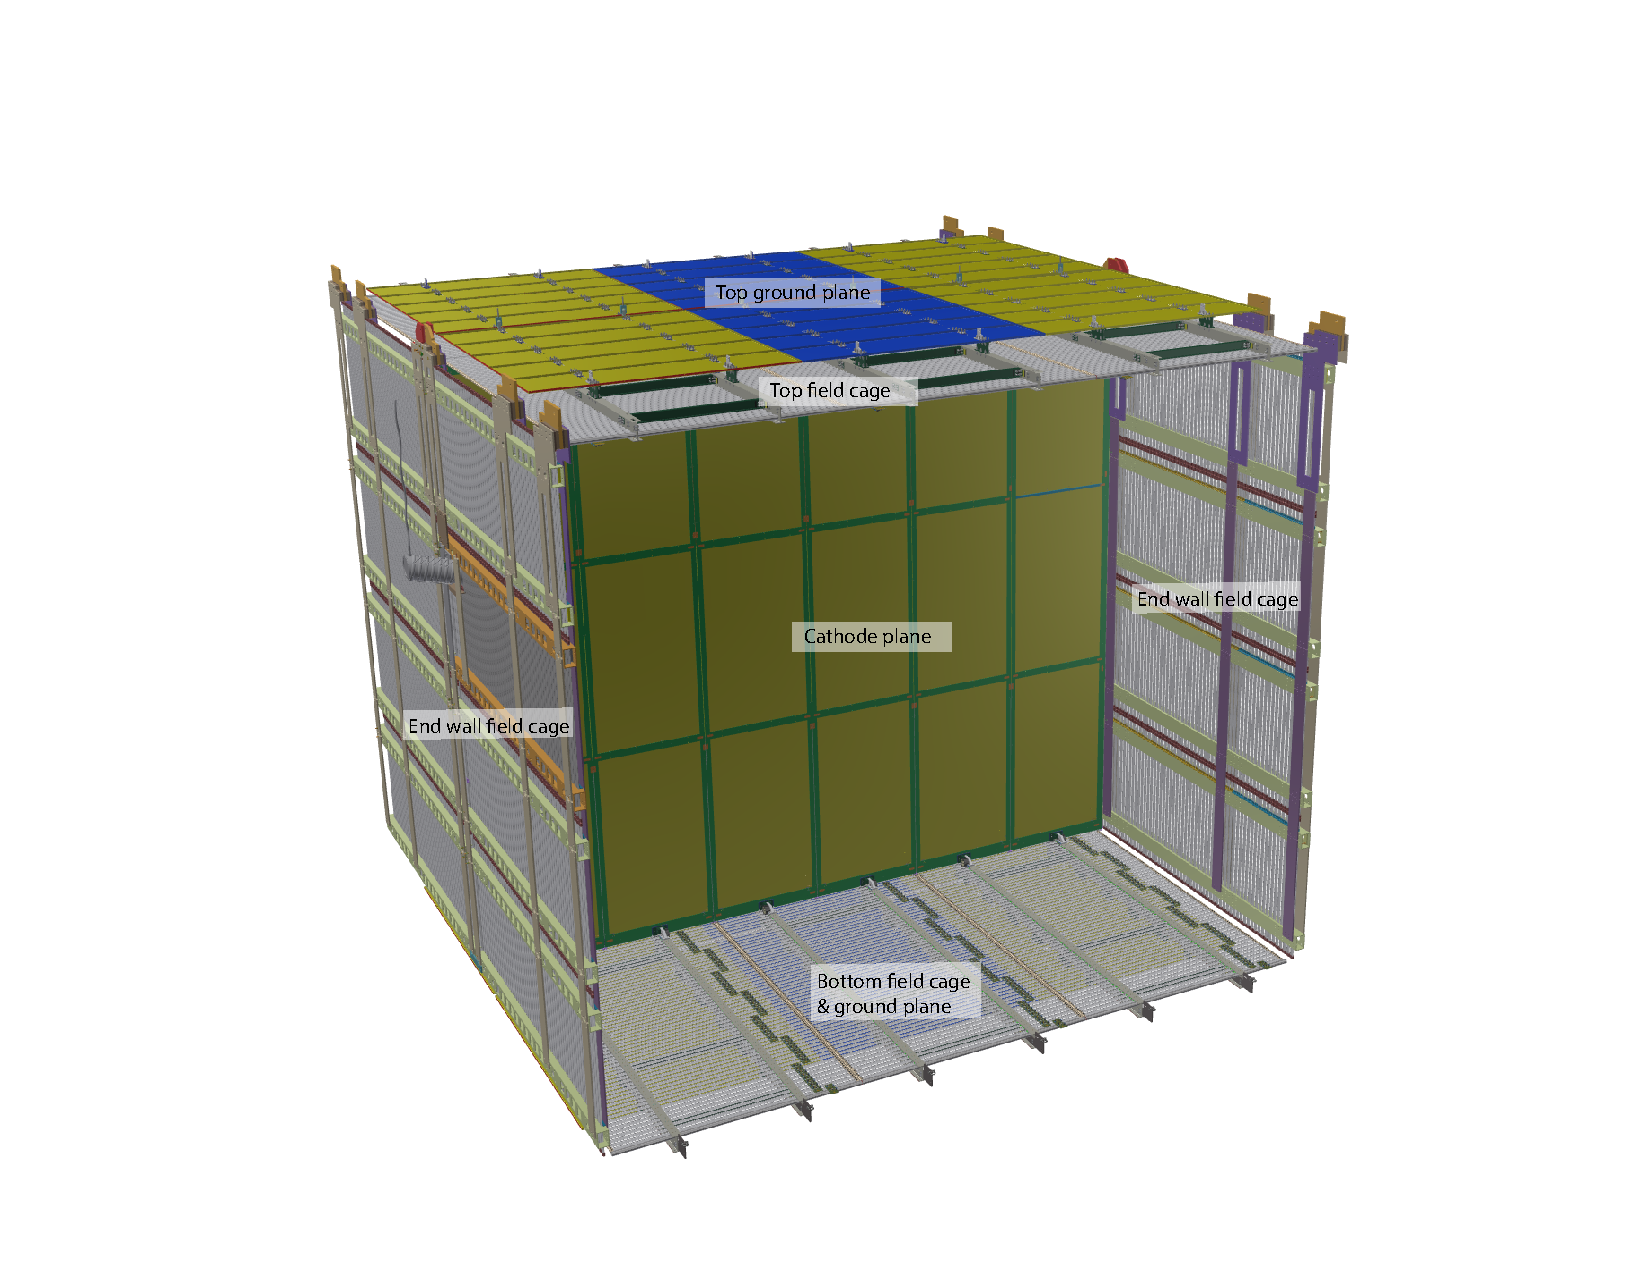
\includegraphics[width=0.8\linewidth]{tpc_fc_overview.png}
\end{cdrfigure}
\fixme{Figure~\ref{fc-overview} is not referenced. It also needs a fuller, more descriptive caption}

The FC is required to:
\begin{itemize}
\item provide the nominal drift field of 500V/cm;
\item withstand $-$180kV near the cathode;
\item define the drift distance between the APAs and CPAs to <1~cm;
\item limit the electric field %exposed to LAr 
in the LAr volume to under 30~kV/cm;
\item miminize the peak energy transfer in case of a HV discharge anywhere on the field cage or cathode;
\item provide redundancy in the resistor divider; \fixme{this feels incomplete... ``in the resistor-divider chain?}
\item maintain the divider current %must be >> 
much greater than the ionization current in the TPC drift cell, yet less than the power supply current limit when all dividers are connected in parallel;
\item %Constructed in 
be modular in form such that they can be easily installed in the cryostat;
\item provide support for the beam plug;
\item allow calibration laser beams to enter into the active volume; 
\item support a 200-lb. person standing on the support beam of the bottom field cage module;
\item be configurable to either 3.6~m or 2.5~m drift length inside the cryostat; and
\item %No 
prevent any trapped volume.

\end{itemize}

%%%%%%%%%%%%%%%%%%%%%%%%%
\subsection{Electrical Design}

Given a large standoff distance between the field cage and the grounded cryostat wall, it is relatively easy to design a field cage that meets the 30-kV/cm E field limit with 180-kV bias.  However, It becomes challenging %if we want 
to reduce the clearance between the FC and ground in order to make more efficient use of liquid argon.  %To achieve this goal, one must look for 
This requires an electrode with a low profile, rounded edges, no trapped volume, and low cost.  Several commercially available roll-formed metal profiles were studied and appear to meet these requirements. \fixme{what's challenging about it then?}


%%%%%%%%%%%%
\subsubsection{Electrostatic analysis}

%One particular profile (
The Dahlstrom Roll Form \#1071 was found to have the lowest surface E field, which was about 12~kV/cm when biased at 180~kV with only a 20-cm ground clearance (see Figure~\ref{fig:fc-profile1071}).

\begin{cdrfigure}[2D FEA of roll formed profiles]{fc-profile1071}{A 2D FEA of a configuration using profile 1071, and a conceptual design of the field cage module}
\includegraphics[width=0.8\linewidth]{tpc_fc_profile1071.png}
\end{cdrfigure}
  
In order to maintain a modular design of the field cage while minimizing peak energy transfer in a discharge,% we chose to construct 
the field cage will be constructed with electrical isolation between neighboring modules. %such that 
If a discharge occurs on one field cage, the %nearby 
electrodes from the neighboring modules will not arc over and cause a domino effect.  This requires a 
electrical insulation between profile ends of the order of 180~kV.  UHMW PE caps of 5-mm thickness are placed over both ends of each profile to serve this purpose. This technique also limits the exposed electric field in LAr at the corner of the field cage, see Figure~\ref{fig:fc_corner}. 

\begin{cdrfigure}[3D FEA of field cage corner]{fc_profile_corner}{A 3D FEA of a field cage corner.  The PE caps (in outline form) limit the exposed E field below the 30kV/cm threshold.}
\includegraphics[width=0.6\linewidth]{tpc_fc_profile_corner.png}
\end{cdrfigure}

The center-to-center distance between the profiles is set to 6~cm, and the inner surface of all profiles on a field cage module is placed 5~cm beyond the nearest surface of the TPC active volume (defined by the APA active aperture over the drift distance). The E field uniformity at the edge of the active volume is expected to be within $\pm$2\% of the nominal value.


%%%%%%%%%%%%  
\subsubsection{Surge suppressor on field cage}

The resistors along the divider provide a linear DC voltage gradient. However, at shorter time scales ($\ll$1~s), the electrical behavior of the divider is determined by the various capacitances on and between each electrode, and %.  This divider
 is no longer linear at this time scale. 

A perfect capacitive divider requires the capacitance of each node to ground to be zero.  In reality, there is always a finite capacitance from each node to ground, and these capacitances resist change in the voltages on the nodes. In the event of a HV breakdown between the cathode %to 
and ground (cryostat), the cathode voltage quickly collapses to ground, but the first FC electrode-to-ground capacitance keeps its voltage from changing instantaneously to follow the cathode voltage, resulting in a momentarily larger voltage differential between the cathode and the first FC electrode. This voltage differential can be a significant fraction of the cathode operating voltage, large enough to cause HV breakdown between the two electrodes, or worse yet, to destroy the divider resistors between the two electrodes.

A natural solution to this problem is to significantly increase the capacitance between the nodes of this divider. This was the approach adopted in the 35-ton prototype's field cage through the use of double-sided printed circuit boards (PCB).  However, the cost of the PCB version of the field cage at DUNE scale is very high, and adding discrete HV capactitors between divider taps is also expensitive.

An alternative is to use surge surpressors in parallel with the divider resistors to divert the transient current from the resistors. Extensive tests have been done by MicroBooNE (docdb 3242, arXiv:1406.5216v2) \fixme{add in bib and cite here} on the use of metal oxide varistors (MOVs) and gas discharge tubes (GDTs) as a means of limiting the over-voltage condition in the event of a HV discharge in the TPC. 

Both types will work for the purpose of restricting the voltage differential between field cage rings in LAr temperature. 
A GDT quickly shorts the terminals when the voltage differential exceeds a threshold, while
a varistor changes its resistance to keep the voltage differential near the threshold voltage.
The smooth transition and well defined clamping voltage of the varistors are preferred to the abrupt switching of the GDTs.
The varistors could also function as redundant ``resistors'' in a divider chain in case a resistor is open circuit. \fixme{open circuited?}

One readily available MOV famility \fixme{family?} with high threshold voltage is the Panasonic ERZ-VXXD182.  These have a threshold voltage around 1600~V.  Two of these in series could work with the current 3-kV differential between divider taps.  However, this configuration would not allow raising the E field much above the nominal 500~V/cm.  To allow some headroom in operating field, three such MOVs in series would be needed.


%%%%%%%%%%%%
\subsubsection{Resister tolerance and specification}

\begin{cdrfigure}[The resistive divider]{fc-divider-view}{A view of a resistive divider}
\includegraphics[width=0.8\linewidth]{tpc_fc_r_divider.png}
\end{cdrfigure}

%%%%%%%%%%%%
\subsubsection{Electrical schematic}
 
\begin{cdrfigure}[Field cage schematic diagram]{fc-schematic}{A schematic diagram of the CPA and a top/bottom field cage module pair}
\includegraphics[width=0.8\linewidth]{tpc_fc_schematic.png}
\end{cdrfigure}

%%%%%%%%%%%%%%%%%%%%%%%%%
\subsection{Validation tests of roll-formed FC design}

A dedicated test setup has been designed and constructed to validate the field cage concept  in purified LAr.
It consists of a field cage (Figure~\ref{fig:fc-test}), fitting into the ICARUS 50-liter cryostat (1.1~m hight, 0.6~m diameter) available at CERN, and  includes:

\begin{itemize}	
\item roll-formed metal profiles with UHMW PE caps,
\item pultruded fiberglass I-beams form four mini panels,
\item HV cable feed-through (equipped with corona monitor) allowing application of up to 150~kV on FC profiles,
\item all profiles at same potential to simplify HV connection,
\item ICARUS-like stainless steel ground planes placed  66~mm away from FC profiles ($\sim$1/3 of FD bias voltage to reach
same E field), and
\item video cameras in the gas phase to monitor bubbles and sparks.
\end{itemize}

\begin{cdrfigure}[The field cage test setup]{fc-test}{The field cage test setup. 
 {\bf Left:} schematic drawings of the cage showing the main elements: metal profiles, I-beams, ground planes.
  {\bf Right:} Picture of the realized setup.}
\includegraphics[width=0.45\linewidth]{tpc_fc-test-1.png}
\includegraphics[width=0.45\linewidth]{tpc_fc-test-2.png}
\end{cdrfigure}

Two choices of material (aluminum, stainless steel) for the metal profiles have been tested. In the aluminum case, the surface finish has also been tested with scratches up to 100 microns deep. 

The cage was operated both in commercial LAr and, connected to the ICARUS 50-liter recirculation system, in LAr with purity  better that 0.1 ppb O$_2$ equivalent. HV above 80~kV (corresponding to an electric field about 20\% higher than nominal) could be 
\fixme{was?} applied for several days, without recording any discharge. Two additional regimes have been studied:
\begin{itemize}	
\item  With the 50-liter vessel fully thermalized (no visible bubble formation along the detector), no sparks appear %(were ever recorded) 
with voltage up to 100~kV.
\item  HV instabilities arise in the 80$-$100 kV range if the LAr is not perfectly thermalized, allowing bubble formation from heat sources (HV feedthrough, ground connections): a few random sparks were recorded, developing however around the HV cable and not between the field cage and the ground plates.
\end{itemize}

All tested materials exhibited the same behavior in the applied HV range. 

Nickel coating (up to 20 microns) of aluminum profiles was also proposed as a way to avoid oxidation of the surface, which % could possibly be 
is a potential source of HV instability. Its stability against  thermal gradients was positively tested. \fixme{tested and found to be positive, i.e, stable? Pls clarify} However HV tests showed no difference with respect to the uncoated version.

A specific breakdown test has been performed to check dielectric rigidity of the UHMW PE end caps in LAr. %exposing a few metal profiles equipped with PE end caps and connected the HV, to a ground plane (Figure~\ref{fig:endcap-test}).
A few metal profiles equipped with PE end caps and connected the HV were exposed to a ground plane (Figure~\ref{fig:endcap-test}).
Results demonstrated that the proposed end-cap geometry and thickness can safely hold 150~kV.

\begin{cdrfigure}[Setup to test dielectric rigidity]{endcap-test}{Setup to test dielectric rigidity of the UHMW PE end caps}
\includegraphics[width=0.65\linewidth]{tpc_fc_endcap-test.png}
\end{cdrfigure}

%%%%%%%%%%%%%%%%%%%%%%%%%
\subsection{Ground Plane Design}
%% by A. Zani

In order to confine the electric field in the liquid argon region, it is foreseen to install a grounded metallic plane,  between the upper field cage module and the liquid-gas interface. The design of such a Ground Plane (GP) \fixme{need to define acronym above and just use it} is inspired by the one from the ICARUS T600 detector, and it is meant to limit the residual electric field in the liquid below the usual 30~kV/cm value. 
\fixme{Is it to keep the E field from going outside the LAr volume or is it to keep the residual field that's already in the LAr volume very small?}
%The design details of the planes were verified to comply with the requests on residual electric field with FEA.  It is noted that a similar GP could be added in front of all the other Field Cage (FC) modules, in order to smooth the field in the LAr dead volume. However, so far it is foreseen to add an actual GP only below the bottom FC, to further smooth the field in the region where pipings for the cryostat filling are running. The distance between the cryostat walls and the end-wall field cage does not require to insert a GP, instead.
The design details of the planes were verified for compliance with the requests on residual electric field with FEA. \fixme{I cannot parse prev sentence} It is noted that a similar GP could be added in front of each of the other Field Cage (FC) modules in order to smooth the field in the LAr dead volume. However, so far it is planned to add one only below the bottom FC, to further smooth the field in the region where pipings for the cryostat filling  run. The distance between the cryostat walls and the end-wall field cage does not require insertion of a GP.

As mentioned, the GP design is inspired by the ICARUS T600 detector: in that case, 1 mm thick Stainless Steel (SS) plates, punched with $10$ mm holes, 15 mm pitch ($\sim 50\%$ transparency), could stand a potential differential of $-150$ kV over $100$ mm. In order to smooth the field, the edges of the planes were rounded to $\sim 10$ mm. The fraction of punched structure was selected to ensure light-weight even with SS, and to allow fluid circulation above the planes.

\fixme{Does this mean: This GP is similar to the one in the ICARUS detector, (the listed features are the same for both). The ICARUS GP can withstand a potential differential of $-150$ kV over $100$ mm, therefore ours can, too.  In  ICARUS, the edges of the GPs were rounded to $\sim 10$ mm, so we plan to do the same?  Is our punched fraction different than ICARUS's because we want it to be lighter-weight or allow more fluid flow? }

In the ProtoDUNE-SP configuration, the GP will be put at a distance of 200~mm from the FC profile, with a structure of $6$ mm holes, $10$ mm pitch ($\sim 25\%$ transparency): the lower fraction of pierced surface is verified by simulations to maintain the field within the required values. The edges of the plates, $20$ mm high, are rounded at $5$ mm, while the holes rounding radius, at production is around $0.5$ mm. The liquid level is expected to be at 40 mm above the GP bottom, i.e. 20 mm above the edges. The radius of curvature for the holes is not a strict requirement. It depends on the punching technique, and usually is at around $0.5$ mm. The actual requirement is to have the hole curvature on the inside (of the TPC) looking out.
\fixme{The previous pgraph needs clarification}

Two sets of pieces \fixme{two sets of GPs? Define ``piece''} were initially produced in Europe:
\begin{itemize}
\item 8 pieces of dimension $198 \times 571$ mm (weight $< 1$ kg each) to be installed in the CERN field cage prototype,
\item 6 more pieces of  $525 \times 2318$ mm (weight around $8.5$ kg each), which represent full scale components for ProtoDUNE-SP. The drawing of this second set of pieces, sent to the U.S. for test assemblies, in shown in Figure~\ref{fig:gp_panels}.
\end{itemize}

\begin{cdrfigure}[ProtoDUNE GP]{gp_panels}{Top: Techincal Drawing, by Claudio Montanari, of the Ground Plane panels for ProdoDUNE-SP. Bottom: 3D model of one panel}
\includegraphics[width=1.0\linewidth]{tpc_fc_gp525x2318piece.png}
\end{cdrfigure}

The choice of electropolished Stainless Steel \textit{AISI 304 L} over Aluminum derives from the experience of the ICARUS detector, moreover:
\begin{itemize}
\item SS and G10 have very similar dilatation coefficients, while Aluminum does not. Choosing SS ensures that all the $GP\,+\,G10$ structure contracts consistently, without too large stresses at the connections; 
\item SS is more ductile than Aluminum, which makes \textit{easier} to machine the corners of the pieces. Note that anyway some imperfections are present even in the SS case, and not all corners will be perfectly identical. 
\item Though Aluminum would guarantee a factor-of-three lighter GP, the overall weight of the SS pieces remains contained (order of 550 kg). \fixme{in other words, SS would also be light enough?}
\end{itemize}

%%%%%%%%%%%%%%%%%%%%%%%%%
\subsection{Field Cage prototype at CERN}
%The main description of the Field Cage Prototype built at CERN, and the tests performed on it, is provided in section ...\fixme{fix}. In here simply the details concerning the GP are reminded. The smaller pieces of GP were installed on the field cage prototype at CERN, to test the configuration. As described elsewhere, the actual distance between the field cage profiles and the GP in this prototype is of 60 mm, therefore a voltage of 60 kV minimum must be attained to verify the ProtoDUNE field configuration. (Figure ~\ref{fig:fc_prot}) During multiple tests in LAr, both with open-air dewars and in a clean liquid configuration, the structure always stood the 60 kV voltage, and it was in general possible to reach the value of 80-100 kV, after which discharges would start. However discharges were always localized on the HV cables, not involving the GP-FC structure.

The main description of the Field Cage Prototype built at CERN, and the tests performed on it, is provided in section ...\fixme{fix}. This section aims to serve as a reminder of the details.
The smaller pieces of the GP were installed on the field cage prototype at CERN to test the configuration. As described elsewhere \fixme{where?} the actual distance between the field cage profiles and the GP in this prototype is of 60~mm, therefore a  minimum voltage of 60~kV must be attained to verify the ProtoDUNE-SP field configuration. (Figure~\ref{fig:fc_prot} \fixme{This figure needs more explanation; what's right and left? where's the 60mm separation?} During multiple tests in LAr, both with open-air dewars \fixme{how do you have LAr in an open dewar?}  and in a clean liquid configuration, the structure consistently withstood the 60 kV voltage, and in fact 80-100 kV was typically achieved, above which discharges would start. The discharges remained localized on the HV cables, and did not involve the GP-FC structure.

\begin{cdrfigure}[CERN Prototype]{fc_prot}{Details of the Field Cage Prototype at CERN, showing the installed GP panels.}
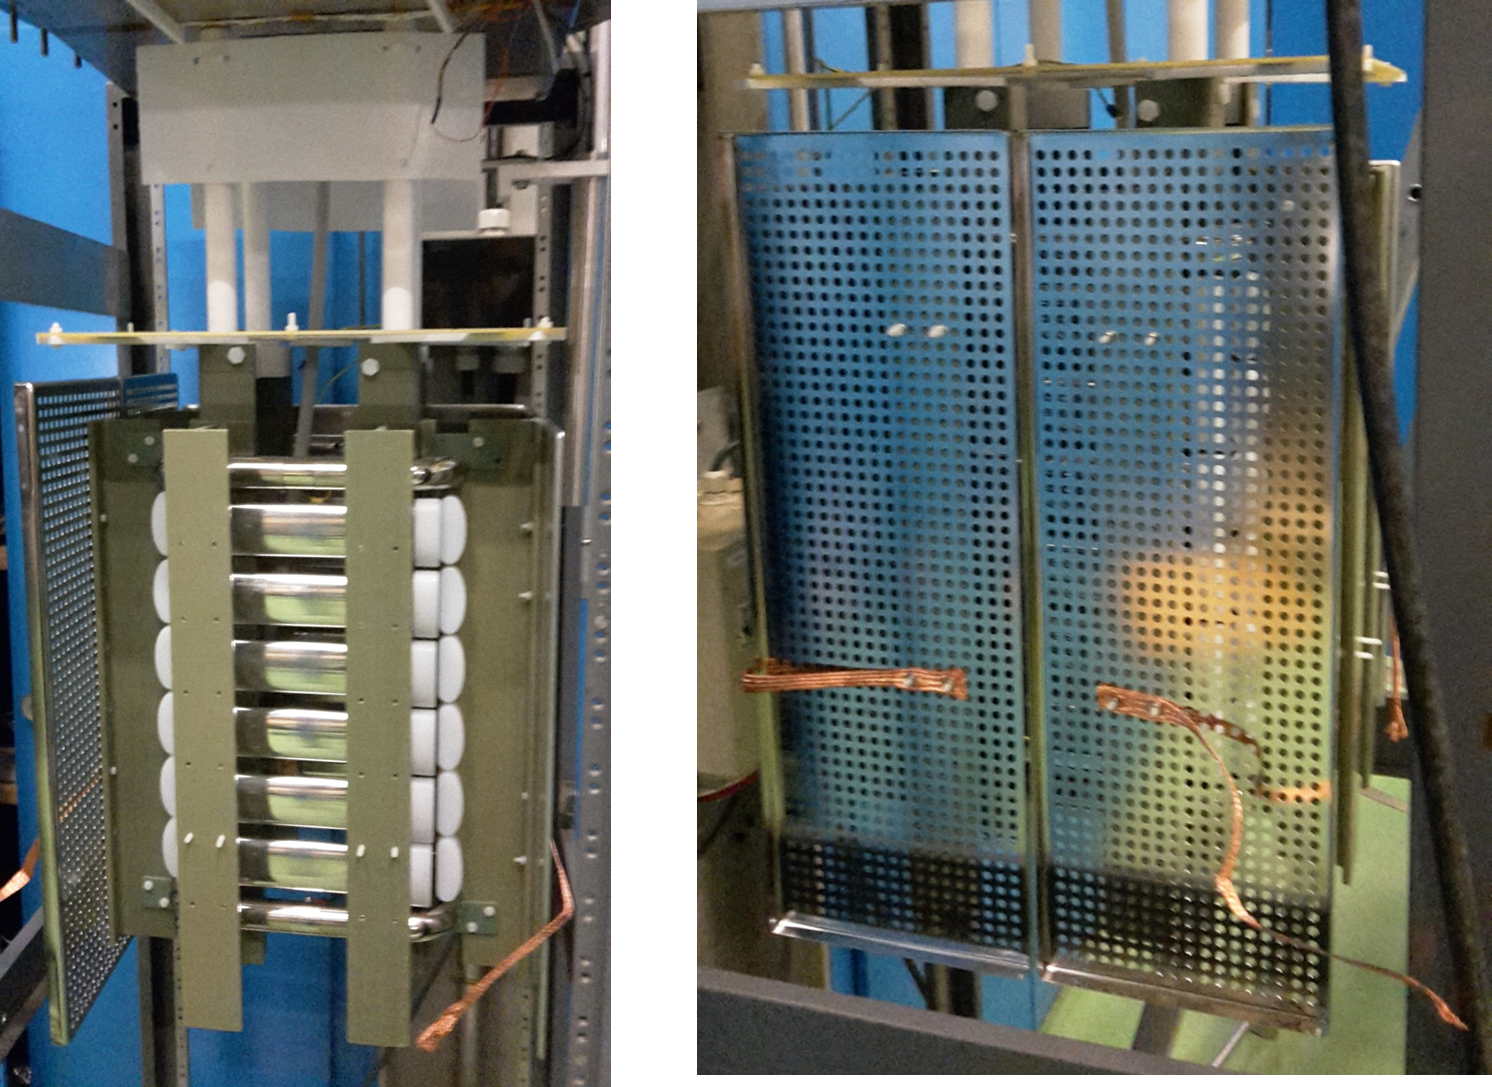
\includegraphics[width=0.8\linewidth]{tpc_fc_prototype.png}
\end{cdrfigure}

%%%%%%%%%%%%%%%%%%%%%%%%%
\subsection{Field Cage and Ground Plane in ProtoDUNE-SP}

The design details of the FC+GP modules for ProtoDUNE is described and shown in the next section. \fixme{add proper reference} Figure~\ref{fig:fc_full} shows a 3D model of one fully assembled module to provide an initial understanding.

\begin{cdrfigure}[CERN Prototype]{fc_full}{3D model of one fully assembled FC+GP module, for the top of the field cage. }
\includegraphics[width=0.8\linewidth]{tpc_topFC.png}
\end{cdrfigure}

One module will be made of six pieces, aligned %put next to each other 
along their long (2318-mm) dimension %direction%: this dimension is made to 
 in order to match the APA and FC module widths. The planes are connected to the FC beam with additional %further 
G10 pieces that are used also to connect adjoining %two neighboring 
GP panels. \fixme{piece vs panel?}

The electrical continuity between consecutive panels can be made %performed 
with metallic screws (with holes on the planes edges) or with looser connections, e.g., copper strips, that better adapt to the shrinking of the structure during cooldown. Copper strips were successfully employed on the CERN FC prototype.
As for most detector systems, the GP should be referenced to the detector ground, located % set 
at the cryostat top.

The GP modules will be installed on the corresponding FC modules in the clean room outside the cryostat, to facilitate the connections. The description of how the top/bottom FC modules are assembled and connected to the CPA before insertion in the cryostat is provided in section ... \fixme{add reference}.

Further GP panels need to be attached to the top FC module:
\begin{itemize}
\item Smaller panels will have to be connected on the modules on one side of the CPA so that, once in position, they %should 
cover the CPA frame. Their dimensions are % is 
still to be defined, depending on the final design of the CPA hanging scheme. Such \fixme{the same pieces are connected, or similar ones are?} pieces should also be connected to the modules covering the opposite drift region, when in final position.
\item An additional % further 
set of small panels should be installed on the outer modules of the FC to extend the GP over the vertical FC walls, which will %to 
further constrain the electric field in these regions. A FEA (Figure ~\ref{fig:fea_overhang}) shows that the optimized overhang distance is 20~cm, provided LAr is at 40~mm above the bottom of the GP. The maximal residual field in this configuration is of the order of 13~kV/cm, with less than 1~kV/cm field in the gas phase.
\end{itemize}

\begin{cdrfigure}[FEA overhang]{fea_overhang}{2D FEA showing the field profile in liquid with a 200-mm overhang, gas-liquid interface 40~mm above the GP bottom. Highest field in the liquid phase is of the order of 13~kV/cm.}
\includegraphics[width=0.7\linewidth]{tpc_fc_gp_overhang.png}
\end{cdrfigure}







%%%%%%%%%%%%%%%%%%%%%%%%%
\subsection{Designs of the Field Cage Modules}

%%%%%%%%%%%%
\subsubsection{Top and bottom modules}


%\begin{cdrfigure}[A top field cage module]{fc-top_module}{A view of a top field cage module}
%\includegraphics[width=0.8\linewidth]{tpc_fc_top_module.png}
%\end{cdrfigure}


%%%%%%%%%%%%
\subsubsection{End wall modules}

\begin{cdrfigure}[An end wall field cage module]{fc-endwall_module}{A view of an end wall field cage module}
\includegraphics[width=0.8\linewidth]{tpc_fc_endwall_module.png}
\end{cdrfigure}


%%%%%%%%%%%%
\subsection{Interfaces to Other TPC Components}

\subsubsection{Field cage to CPA}

On the top and bottom of the TPC, hinges connect each field cage module to two CPA columns.  This design allows the field cage modules to be pre-attached to the CPAs during installation, and prevents accidental damage to the APA wire plane when raising the field cage module to connect %link 
to the APA.

The end-wall field cage modules are hung from the CPA and APA support rails.  They do not have strong mechanical coupling to the CPAs and APAs, however, at least four resistive divider chains must be connected to the CPA's HV bus.

\begin{cdrfigure}[CPA to field cage connection]{cpa-fc-connection}{A top field cage module connected to two CPA modules}
\includegraphics[width=0.8\linewidth]{tpc_fc_cpa_connection.png}
\end{cdrfigure}


%%%%%%%%%%%%
\subsubsection{Field cage to APA}

The I-beams of the top/bottom field cage modules are designed to be latched onto the mating brackets on the APAs.  The design details are currently being developed. % at this moment.  
In addition to the mechanical connection, the ground side of the divider chain must be connected to the APA's frame ground. % as well.


%%%%%%%%%%%%
\subsubsection{Field cage to beam plug}

The design of the beam plug is described in Section~\ref{sec:beamplug}. In this section we describe the interface between the beam plug and the field cage. The beam plug is installed between the field cage and primary membrane where the charged particle beam enters the cryostat. Its main function is to displace about 45 cm of passive LAr layer in that region to allow the particle beam to enter the active TPC region with minimal upstream material interactions. The beam plug is mounted onto one of the field cage support structures as shown in Figure~\ref{fig:fc-beamplug}.
\begin{cdrfigure}[Beam plug to CPA connection]{fc-beamplug}{Beam plug to CPA connection}
\includegraphics[width=0.5\linewidth]{fc-beamplug.jpg}
\end{cdrfigure}


%%%%%%%%%%%%
%% this feature has been removed from ProtoDUNE design
%\subsubsection{Field cage to calibration lasers}

%Four calibration laser windows need to be implemented on the downstream end-wall field cage modules.  The windows are planned to be at the mid-height of the TPC, i.e., at the boundary of two %end-wall field cage 
%modules.  The opening for each laser beam is about 15~cm square.  The plan is to shorten three profiles by 7.5~cm from the each edge of the field cage modules.



%%%%%%%%%%%%%%%%%%%%%%%%%
\subsection{QC Procedures}

The following activities are/will be performed to assure the field cage meets all design criteria as defined in the fabrication drawings and description in the sections above:
\begin{itemize}
\item	Fabricate prototype FCs to test the design and fabrication and assembly methods.
\item	Installation test at Ash River:
\begin{itemize}
\item	Test the lifting and handling of the prototype FCs.
\item	Mount the prototype FCs to the CPA modules and test and evaluate their installation.
\end{itemize}
\item	Develop a QC plan for inspecting every fabricated part of the FC frame to make sure they meet the dimensions and tolerances on the fabrication drawings.
\item	Develop a QC plan for inspecting and measuring each FC module and completed FC plane to insure they meet the dimensions and tolerances on the drawings.
\item	Perform tests of each joint in the FC frame (see Section XX) to insure that their design and strength meets the load requirements.
\item	Create an integrated model of the entire TPC to evaluate interfaces and installation methods.  
\end{itemize}

 



%\chapter{det-comp}


%%%%%%%%%%%%%%%%%%%%%%%%%%%%%%%%%%%%%%%%%%%%%%
%\section{Anode Plane Assemblies}

%%%%%%%%%%%%%%%%%%%%%%%%%%%%%%%%%%%%%%%%%%%%%%
%\section{Cathode Plane Assemblies}

%%%%%%%%%%%%%%%%%%%%%%%%%%%%%%%%%%%%%%%%%%%%%%
%\section{Field Cage}

%%%%%%%%%%%%%%%%%%%%%%%%%%%%%%%%%%%%%%%%%%%%%%
\section{HV components}

%\chapter{det-comp}


%%%%%%%%%%%%%%%%%%%%%%%%%%%%%%%%%%%%%%%%%%%%%%
%\section{Anode Plane Assemblies}

%%%%%%%%%%%%%%%%%%%%%%%%%%%%%%%%%%%%%%%%%%%%%%
%\section{Cathode Plane Assemblies}

%%%%%%%%%%%%%%%%%%%%%%%%%%%%%%%%%%%%%%%%%%%%%%
%\section{Field Cage}

%%%%%%%%%%%%%%%%%%%%%%%%%%%%%%%%%%%%%%%%%%%%%%
%\section{HV components}

%%%%%%%%%%%%%%%%%%%%%%%%%%%%%%%%%%%%%%%%%%%%%%
\section{TPC Front-end Electronics}
%\chapter{Cold Electronics}
\label{ch:ce}

%
%%%%%%%%%%%%%%%%%%%%%%%%%%%%%%%%
%\subsection{Introduction}
\subsection{Scope and requirements}
\label{subsec:ce_intro}


The DUNE single-phase TPC read-out electronics are referred to as the ``Cold Electronics'' (CE) because they reside in LAr,
mounted directly on the APA, as shown in Figure~\ref{fig:tpcce_FEMBonAPA}, thus reducing channel capacitance and noise by minimizing the length of the connection between an anode wire
and its corresponding electronics input.

\begin{cdrfigure}[The front-end electronics mounted on an APA]{tpcce_FEMBonAPA}{The 
front-end electronics as mounted on an APA.
  Top: The front-end electronics is shown in the red circle.
 Bottom: Cross section view showing the layered wire boards. Mounting hardware between the front-end electronics 
and the APA is not shown.}
\includegraphics[width=0.8\linewidth]{tpcce_CMBonAPA_1.pdf}
\includegraphics[width=0.8\linewidth]{tpcce_CMBonAPA_2.pdf}
\end{cdrfigure}

The CE signal processing is implemented in ASIC chips using CMOS technology,
which has been demonstrated to perform well at cryogenic temperatures,
and includes amplification, shaping, digitization, buffering, and multiplexing (MUX) of the signals.
The CE is continuously read out,
resulting in a digitized ADC sample from each APA channel (wire) up to every 500\,ns (2-MHz maximum sampling rate). 

The 2,560 channels from each APA are read out by 20 Front-End Motherboards (FEMBs), each providing 
digitized wire read-out from 128 channels. One cable bundle 
connects each FEMB to the outside of the cryostat via a feedthrough (a \textit{CE feedthrough}) in the signal cable flange at the top of the cryostat, where a single flange services each APA, as shown in Figure~\ref{fig:tpcce_apa_flange}. 
Each cable bundle contains wires for low-voltage (LV) power, high-speed data readout,
and clock/digital-control signal distribution.
Eight separate cables carry the TPC wire-bias voltages from the signal flange to the APA wire-bias boards, as
shown schematically in Figure~\ref{fig:tpcce_cr_board}.

\begin{cdrfigure}[Connections between signal flange and APA]{tpcce_apa_flange}{Connections between
the signal flange and APA.}
\includegraphics[width=0.4\linewidth]{tpcce_apa_flange.pdf}
\end{cdrfigure}

The components of the CE system are the:
\begin{itemize}
\item Front-end mother boards (FEMBs), which house the cold ASICs and are installed on the APAs;
\item Cables for the data, clock/control signals, LV power, and wire-bias voltages 
between the APA and the signal flanges (cold cables);
\item Signal flanges with a CE feedthrough to pass the data, clock/control signals, 
LV power, and APA wire-bias voltages between the inside and outside of the cryostat;
\item Warm interface electronics crates (WIECs) that are mounted on the signal flanges and contain the warm interface boards (WIBs)
and Power and timing cards (PTCs) for further processing and distribution of the signals entering/exiting the cryostat;
\item Fiber cables for transmitting data and clock/control signals between the WIECs and the data acquisition 
(DAQ) and slow control systems;
\item Cables for LV power and wire-bias voltages between the signal flange and external power supplies (warm cables); and
\item LV power supplies for the CE and bias-voltage power supplies for the APAs.
\end{itemize}

The electrical cables for each APA enter the cryostat through a single 
signal flange, creating an integrated unit that provides local diagnostics for noise and validation testing,
and follows the grounding guidelines in Section~\ref{subsec:groundshield}. The components, the quantity of each required for ProtoDUNE-SP, and the number of channels that each component has, are listed in Table~\ref{tab:ce-components}.

\begin{cdrtable}[Electronics components and quantities]{llr}{ce-components}{Electronics components and quantities}
Element                                                             &  Quantity                                  &  Channels per element   \\  \toprowrule
TPC                                                                   & 1                                               & 15,360    \\  \colhline
APA                                                                   & 6                                               & 2,560     \\  \colhline
Front-End Mother Board (FEMB)                         & 120, 20 per APA                       & 128     \\  \colhline
%\hspace{0.02\textwidth} 
FE ASIC chip                                & 120 $\times$ 8, 8 per FEMB      & 16          \\   \colhline
ADC ASIC chip                             & 120 $\times$ 8, 8 per FEMB      & 16          \\   \colhline
FEMB FPGA                                  & 120, 1 per FEMB                         & 128          \\   \colhline
Cold cable bundles                     & 120, 1 per FEMB                        & 128      \\   \colhline
Signal flange                                & 6, 1 per APA                              & 128 $\times$ 20  (i.e., 2,560)  \\   \colhline
CE feedthrough                            & 6, 1 per APA                             &128 $\times$ 20         \\   \colhline
Warm interface boards (WIB)         & 30, 5 per APA                             & (128 $\times$ 20) /5 (i.e., 512)        \\   \colhline
 Warm interface electronics crates (WIEC)     & 6, 1 per APA                             & 128 $\times$ 20         \\   \colhline
 Power and timing cards (PTC)       & 6, 1 per APA                             & 128 $\times$ 20         \\   \colhline
Passive backplane (PTB)                & 6, 1 per APA                             & 128 $\times$ 20 \\   \colhline
LV power mainframe               & 2                        &   7,680   \\    \colhline
LV supply modules          &  6, 1 per APA       &  128 $\times$ 20            \\    \colhline
Wire-bias mini-crate               & 2                        &   7,680   \\    \colhline
Wire-bias supply modules    & 6, 1 per APA                        &   128 $\times$ 20   \\
\end{cdrtable}

The most significant requirements for the CE are listed here. The CE shall:

\begin{itemize}	
\item Provide the means to read out the TPC wires and transmit their data in a useful format to the DAQ;
\item Operate for the life of the facility without significant loss of function;
\item Dead or unusable channels at $<$~1$\%$, causing $>$~97$\%$ of the fiducial volume to be observed by all 3 active wire planes;
\item Record the channel waveforms continuously without dead time;
\item Be constructed only from materials that are compatible with high-purity LAr;
\item Provide sufficient precision and range in the digitization to:
\begin{itemize}
\item Discriminate electrons from photon conversions;
\item Optimize the reconstruction of high- and low-energy tracks from accelerator-neutrino interactions;
\item Distinguish a Minimum Ionizing Particle (MIP) from noise with a signal-to-noise ratio $>$ 9:1; and
\item Measure ionization up to 15 times that of a MIP particle, so that stopping kaons from proton decay can be identified;
\end{itemize}
\item Ensure that all power supplies have: 
\begin{itemize}
\item Local monitoring and control;
\item Remote monitoring and control through DAQ; and
\item Over-current and over-voltage protection circuits;
\end{itemize}
\item And ensure that the CE feedthroughs are able to withstand twice their nominal operating voltages 
with a maximum specified leakage current in 1-atm argon gas.
\end{itemize}


%%%%%%%%%%%%%%%%%%%%%%%%%%%%%%%%
\subsection{Grounding and shielding}
\label{subsec:groundshield}

To avoid structural ground loops, the APA frames described in Section~\ref{subsec:apa_frame} 
are insulated from each other. Each frame is electrically connected to the cryostat at a single 
point on the CE feedthrough board in the signal flange where the cables exit the cryostat. Mechanical suspension of the APAs 
is accomplished using insulated supports. 

The analog portion of the FEMB contains eight front-end (FE) ASICs configured as 16-channel 
digitizing charge amplifiers. Input amplifiers on the ASICs have their ground terminals connected 
to the APA frame.  All power-return leads and cable shields 
are connected to both the ground plane of the FEMB and to the signal flange.

Filtering circuits for the APA wire-bias voltages are locally referenced to the ground plane of the FEMBs through low-impedance 
electrical connections. This approach ensures a ground-return path in close proximity to the 
bias-voltage and signal paths. The close proximity of the current paths minimizes the size of potential loops to further 
suppress noise pickup.

Photon detector signals, described in Section~\ref{sec:pd_system}, are carried directly on shielded, 
twisted-pair cables to the signal flange. The cable shields are connected to the 
cryostat at a second feedthrough, the PDS feedthrough, and to the PCB shield layer on the photon detectors. There is no 
electrical connection between the cable shields and the APA frame except at the signal flange.

The frequency domain of the TPC wire and photon detector signals are separate. The wire readout digitizes at 2~MHz 
with $<$~500~kHz bandwidth at 1 $\mathrm{\mu}$sec peaking time, while the photon readout operates at 150~MHz 
with $>$~10~MHz bandwidth. They are separated from the clock frequency (50~MHz) and common noise frequencies 
through the FE ASIC and cabling designs. All clock signals are transmitted differentially with individual shield 
to avoid the interference to power lines. 

%
%%%%%%%%%%%%%%%%%%%%%%%%%%%%%%%%
\subsection{Distribution of APA wire-bias voltages}
\label{subsec:ce_wire_bias}

Each side of an APA includes four wire layers as described in Section~\ref{sec:apa-design-overview}. 
The innermost X-plane layer of wires is nominally biased at +820 Volts, with each wire AC coupled 
to one of the 128 charge amplifier circuits on the FEMB. The V-plane wire layer is effectively biased at zero volts, 
with each wire directly connected to one of the charge amplifier circuits. The U-plane wire layer is nominally 
biased at $-$370 Volts with each wire AC-coupled 
to one of the 128 charge amplifier circuits. The outermost G-plane wire layer,
which has no connection to the charge amplifier circuits, is biased at $-$665 Volts.

Electrons passing through the wire grid must drift unimpeded until they reach the X-plane 
collection layer. The nominal bias voltages are predicted to result in this electrically 
transparent configuration.

As described in Section~\ref{subsubsec:apa_wire_anchor}
 the filtering of wire-bias voltages and AC coupling of wire signals passing
onto the charge amplifier circuits is done on Capacitance-Resistance (CR) boards that plug in between the APA wire-board stacks and FEMBs.
Each CR board includes single R-C filters for the X- and U-plane wire-bias voltages. In addition, each board has 48 
pairs of bias resistors and AC coupling capacitors for X-plane wires, and 40 pairs for the U-plane wires. The coupling capacitors block DC while passing AC 
signals to the CE motherboards.

\begin{cdrfigure}[APA wire bias schematic diagram]{tpcce_cr_board}{APA wire bias 
schematic diagram, including the Capacitance-Resistance (CR) board.}
\includegraphics[width=0.9\linewidth]{tpcce_cr_board.pdf}
\end{cdrfigure}

Separate CR boards include a single R-C filter for the G-plane wires and 12 pairs of bias resistors and
coupling capacitors.
Groups of four wires are tied together to share single
bias resistors and filter capacitors. These CR boards do not connect to the charge amplifier circuits on the FEMB.

Clamping diodes limit the input voltage received at the amplifier circuits to between 1.8V~$\pm$~U$\_$D, where U$\_$D
is the breakdown voltage of the diode $\sim$0.7V.
The amplifier circuit has a 22-nF coupling capacitor at input to avoid leakage current from the protection clamping diodes. 

Coupling capacitors for the X-plane and U-plane wires are required to block DC bias voltages.
However they also impact the efficiency of the detector circuits.
The sense wires are expected to have $\sim200$~pF of capacitance to the APA frame.
Induced or collected charges are effectively divided between the wire capacitance and the coupling capacitor.
To achieve a charge-calibration accuracy of 0.5 percent or better,
the coupling capacitors must be 4.7\,nF at ten percent tolerance, or 2.2\,nF at five percent tolerance.
Voltage ratings should be at least 1.5 times the expected operating voltages.

Bias resistance values should be at least 20\,M$\Omega$ to maintain negligible noise contributions.
A target value of 50\,M$\Omega$ is desired.
The higher value helps to achieve a longer time constant for the high-pass coupling networks.
Time constants should be at least 25 times the electron drift time so that the undershoot in the digitized waveform
is small and easily correctable.
However, leakage currents can develop on PC boards that are exposed to high voltages over extended periods.
If the bias resistors are much greater than 50\,M$\Omega$, leakage currents may affect the bias voltages applied to the wires.

The bias-voltage filters are R-C low-pass networks.
Resistance values should be much smaller than the bias resistances to control crosstalk between wires
and limit the voltage drop if any of the wires becomes shorted to the APA frame.
A value around 2.2\,M$\Omega$ is desired.
Smaller values may be considered although a larger filter capacitor would be required to maintain a given level of noise reduction.
A target value of 47\,nF has been established for the filter capacitors.

For the grid-plane bias filters, component values are less critical.
If possible they will be identical to those used for the bias resistors and coupling capacitors
(50~M$\Omega$ and 2.2 to 4.7\,nF).


%%%%%%%%%%%%%%%%%%%%%%%%%%%%%%%%
\subsection{Front-End Mother Board}
\label{subsec:fe_arch}

The main component of the CE architecture, illustrated in Figure~\ref{fig:tpcce_schem}, is the 
128-channel FEMB, which itself consists of an analog motherboard and an attached FPGA 
mezzanine card for processing the digital outputs.
Each APA is instrumented with 20 FEMBs, for a total of 2,560 channels per APA.
The FEMBs plug directly into the APA CR boards, making the connections from the U- and V-plane induction wires and 
X-plane collection wires to the charge amplifier circuits as short as possible.

The analog mother board is instrumented with eight 16-channel FE ASICs,
eight 16-channel ADC ASICs, LV power regulators, and input-signal protection circuits.
The 16-channel FE ASIC provides amplification and pulse shaping.
The 16-channel ADC ASIC comprises  12-bit digitizers performant at speeds up to 2 MS/s, local buffering,
and an 8:1 MUX stage with two pairs of serial readout lines in parallel.

 
   (Figure~\ref{fig:tpcce_CMBpix}).
% following pgraph moved up 9/27   
Each FE ASIC channel has a charge amplifier circuit with a gain selectable from one of 4.7, 7.8, 14 and 25~mV/fC
(full scale charge of 55, 100, 180 and 300~fC),
a high-order anti-aliasing filter with adjustable time
constant (peaking time 0.5, 1, 2, and 3 $\mathrm{\mu}$s),
an option to enable AC coupling,
and a baseline adjustment for operation with either the collecting (200~mV) or the non-collecting (900~mV) wires.
Shared among the 16 channels in the FE ASIC are the bias circuits, programming registers,
a temperature monitor, an analog buffer for signal monitoring, and the digital interface.
The estimated power dissipation of FE ASIC is about 6~mW per channel at 1.8~V supply.

The FE ASIC layout is shown in Figure~\ref{fig:tpcce_ADC_ASIC}.
The ASIC was implemented using the commercial CMOS process (0.18~$\mu$m and 1.8~V), which 
is expected to be available for at least another 10~years. 
The charge amplifier input MOSFET is a p-channel biased at 2~mA with a L/W (channel length/width) ratio
of 0.27~$\mu$m / 10~$\mu$m, followed by dual cascade stages.
The charge amplification and shaping filter have digitally programmable gain and peaking time
(as specified in Section~\ref{subsec:fe_arch}).
Each channel also implements a high-performance output driver,
which can be used to drive a long cable, but is disabled when interfaced to an ADC ASIC to reduce the power consumption.
The ASIC integrates a band-gap reference (BGR) to generate all the internal bias voltages and currents.
This guarantees a high stability of the operating point over a wide range of
temperatures, including cryogenic.
The ASIC is packaged in a commercial, fully encapsulated plastic QFP 80 package.

Prototypes have been evaluated and characterized at RT (300~K) and LN2 (77~K) temperature.
During testing the circuits have been cycled multiple times
between the two temperatures and operated without any change in performance.
Figure~\ref{fig:tpcce_shaper_out} shows the measured pulse response, both as a function
of temperature and the programmable settings of the chip.
These results are in close agreement with simulations and indicate
that both the analog and the digital circuits and interface operate as
expected in a cryogenic environment.

\begin{cdrfigure}[Measured pulse response with details]{tpcce_shaper_out}{Measured pulse response with
 details on gain, peaking time and baseline adjustments}
\includegraphics[width=\linewidth]{tpcce_shaper_out.pdf}
\end{cdrfigure}

\begin{cdrfigure}[Measured ENC vs filter time constant]{tpcce_enc}{
Measured ENC vs filter time constant from the latest prototype version of the FEMB
for two different gains, 14~mV/fC and 25~mV/fC. RT = room temperature and 
LN2 = liquid nitrogen}
\includegraphics[width=0.45\linewidth]{tpcce_enc_14mV.jpg}
\includegraphics[width=0.45\linewidth]{tpcce_enc_25mV.jpg}
\end{cdrfigure}

Figure~\ref{fig:tpcce_enc} shows the measured Equivalent Noise Charge (ENC) as a function of 
filter-time constant (peaking time) for two different gains, where ENC is the value of charge 
(in electrons) injected across the detector capacitance that would produce at the output of the 
shaping amplifier a signal whose amplitude equals the output R.M.S. noise. These measurments
were made with prototype FEMBs at both RT and submerged in LN2 with a wire-simulating input capacitance of $C_f~=~150$~pF.
In LN2, for peaking times $>$1~$\mu$s, less than 600~e$^{-}$ was measured. For comparison,
a MIP travelling perpendicularly to the wire plane in the direction of wire spacing is
expected to deposit $\sim$~10,000~e$^{-}$ on the collection wires, for a worst-case
S:N$\sim$16:1.

Each channel is equipped with an injection capacitor which can be used
for test and calibration and can be enabled or disabled through a
dedicated register. The injection capacitance has been measured using 
a calibrated external capacitor. The measurements show
that the calibration capacitance is extremely stable, changing from
184~fF at RT to 183~fF at 77~K. This result and the measured
stability of the peaking time demonstrate the high stability of the
passive components as a function of temperature. Channel-to-channel and chip-to-chip
variation in the calibration capacitor are typically less than 1\%. 

The ADC ASIC design is also implemented using the CMOS process (0.18~$\mu$m and 1.8V).
The layout of the ADC ASIC is shown in Figure~\ref{fig:tpcce_ADC_ASIC}. 
The ADC ASIC is a complex design with 320,000 transistors, while the FE ASIC has 16,000.
The transistor design work has been done following the rules for long cryo-lifetime.
Shared among the 16 channels in the ADC ASIC are the bias circuits, programming registers,
an 8:1 MUX, and the digital interface.
The estimated power dissipation of FE ASIC is below 5~mW per channel at 1.8~V supply.
  

\begin{cdrfigure}[The layout of the 16-channel ADC ASIC]{tpcce_ADC_ASIC}{The layout of the 16-channel ADC ASIC}
\includegraphics[width=\linewidth]{tpcce_ADC_ASIC_pinout.jpg} % New one
\end{cdrfigure}

The ADC ASIC has an input buffer with offset compensation to match the output of the FE ASIC.
The input buffer first samples the input signal (with a range of 0.2~V to 1.6~V),
then provides a current output after compensating for offset voltage error.
This current output is then supplied to the ADC which converts the input to digital in two phases.
The MSB (Most Significant Bit) 6~bits are first determined followed by the LSB (Least Significant Bit) 6~bits.
After the conversion the thermometer code is converted to binary and latched.
The output of ADC channel 16 can be monitored externally.
The data from the 16 ADCs are transferred in parallel to the FIFO block.
The built-in FIFO is 32~bits wide and 192~bits long,
and has full and empty indicator flags, needed for interfacing to the FPGA.
The ADC along with the input buffers are biased internally using a bias generator and a bandgap voltage reference.
The bandgap voltage (VBGR) can be monitored and/or controlled externally.
It can be put in the low-power sleep mode, and woken up in less than 1~$\mu$s.

Prototypes have been evaluated and characterized at RT (300~K) and LN2 (77~K) temperature.
During these tests the circuits have been temperature-cycled multiple times.
The effective resolution with reference to the input referred noise is $\sim$11.6~bits at both 300~K and 77~K.
The differential non-linearity (DNL) is less than 4 LSBs for 99\% of ADC bins at both 300~K and 77~K.

 
 
 The ADC outputs are passed to the FPGA mezzanine board for transmission to the warm electronics
 located on the outside of the signal flange.
The FPGA has four 4:1 MUX circuits that combine the 16 serial lines from the eight ADC
channels into four serial lines of 32 channels each, and 
four $\sim$1.2 Gigabit-per-second (Gbps) serial drivers that drive the data in each
line over cold cables to the WIBs.

\begin{cdrfigure}[The CE Architecture]{tpcce_schem}{The CE Architecture. The basic unit is the 128-channel FEMB.}
\includegraphics[width=0.9\linewidth]{tpcce_schem.pdf}
\end{cdrfigure}

\begin{cdrfigure}[The Front End Mother Board (FEMB), as used in an early set of tests]{tpcce_CMBpix}
{The Front End Mother Board (FEMB), as used in the early set of tests.
  {\bf Top:} The analog mother board, showing four ADC ASICs and four FE ASICs surface mounted.
  The other side of the board has another four ADC and FE ASICs.
  Except for anticipated small modifications, this board is essentially the final version.
  {\bf Middle:} The FPGA mezzanine, used in place of the digital ASIC mezzanine for the early set of tests.
  {\bf Bottom:} The complete FEMB assembly as used in the early set of tests.
  The cable shown in the high-speed data, clock, and control cable.}
\includegraphics[width=0.65\linewidth]{tpcce_CMBpix_1.pdf}
\includegraphics[width=0.65\linewidth]{tpcce_CMBpix_2.pdf}
\includegraphics[width=0.45\linewidth]{tpcce_CMBpix_3.pdf}
\end{cdrfigure}

The data are passed through the signal flange to the WIBs on copper cables utilizing LV differential signaling (LVDS).
On the WIBs, the data is further MUXed by 4:1 and transmitted over optical
fibers to the DAQ system described in Section~\ref{sec:DAQ_online_interface}.

The FPGA on the mezzanine card is also responsible for communicating with the
DAQ and timing systems and providing the clock and control signals required by the FE and ADC ASICs. 
By default the cold FPGA will load firmware from a cold flash onboard the FEMB. The remote update of 
FPGA firmware via JTAG chain is available through the WIB, with 4 differential cables to each FEMB 
from the WIB. In addition, the cold flash can be programmed remotely. In the case that faulty firmware 
is identified in-situ by slow control and monitoring, an update of the firmware will be initiated.

Each FEMB is enclosed in a Faraday box to provide shielding from noise. 
As shown in Figure~\ref{fig:tpcce_box}, the Faraday box is designed to make the electrical connection 
between the FEMB and the APA frame. %, as defined in Section~\ref{subsec:ele_design}. Not sure what section to reference.
 Mounting 
hardware inside the Faraday box connects the ground plane of the FEMB to the box casing. The
box casing is electrically connected to the APA frame via twisted conducting wire (not 
shown in Figure~\ref{fig:tpcce_box}). This is the only point of contact between the FEMB and
APA, except for the input amplifier circuits connected to the CR board, which also terminate to
ground at the APA frame, as shown in Figure~\ref{fig:tpcce_cr_board}.

\begin{cdrfigure}[Faraday box for the FEMB]{tpcce_box}{Faraday box for the FEMB.}
\includegraphics[width=3in]{tpcce_box_1.pdf}
\includegraphics[width=3in]{tpcce_box_2.pdf}
\end{cdrfigure}

%
%%%%%%%%%%%%%%%%%%%%%%%%%%%%%%%%
\subsection{CE feedthroughs and cold cables}
\label{subsec:ce_feedthrough}

All cold cables originating from inside the cryostat connect to the outside warm electronics through PCB board feedthroughs
installed in the signal flanges that are distributed along the cryostat roof (Figure~\ref{fig:tpcce_FT_InternalCableRoute}).
The TPC data rate per APA, with an overall 32:1 MUX and 80 $\sim$1~Gbps data channels per APA,
is sufficiently low that the LVDS signals can be driven over copper twin-axial transmission lines.
Additional transmission lines are available for the distribution of LVDS clock signals and I$^2$C control information,
which are transmitted at a lower bit rate.
Optical fiber is employed externally from the WIBs on the signal flange to the DAQ and slow control systems.

\begin{cdrfigure}[Conceptual design of CE feedthrough]{tpcce_FT_InternalCableRoute}{
The CE feedthrough configuration and internal cable routing. The left panel shows a cutaway view of the cryostat.
The right panel shows more detail at the Faraday boxes.}
\includegraphics[width=7in]{tpcce_FT_InternalCableRoute.pdf}
\end{cdrfigure}


\begin{cdrfigure}[Conceptual design of CE feedthrough]{tpcce_signal_FT}{
TPC CE feedthrough. The WIBs are seen edge-on in the left panel,
and in an oblique side-view in the right panel, which also shows the warm crate for a DUNE module in a cutaway view (for 
ProtoDUNE-SP, there is a crate only on one side).}
\includegraphics[width=0.6\linewidth]{tpcce_signal_FT.pdf}
\end{cdrfigure}

The design of the signal flange includes a T-shaped pipe, separate PCB feedthroughs for the CE and PDS cables, and
an attached crate for the TPC warm electronics, as shown in Figure~\ref{fig:tpcce_signal_FT}.
The wire-bias voltage cables connect to standard SHV (safe high voltage) connectors machined directly into the CE feedthrough,
ensuring no electrical connection between the wire-bias voltages and other signals passing through the signal flange.
Each CE feedthrough serves the bias/power/digital IO needs of one APA, as shown 
in Figure~\ref{fig:tpcce_cable_routing}.  

\begin{cdrfigure}[TPC cable routing scheme]{tpcce_cable_routing}{TPC cable routing scheme for three APA section.}
\includegraphics[width=0.9\linewidth]{tpcce_cable_routing.pdf}
\end{cdrfigure}

A program for minimizing potential contamination of the LAr from the cable plant contained within the ullage
(the warmer gas phase at the top of the cryostat) 
is being carefully followed.


Data/control cable bundles are used to send system clock and control signals from the 
signal flange to the FEMB, stream the $\sim$1~Gbps high-speed data from the FEMB to the signal flange, and 
provide backup JTAG programming to the cold FPGA, in case the power-up programming from the onboard 
flash EEPROM fails. As described in Section~\ref{subsec:ce_intro}, each FEMB 
connects to a signal flange via one data cable bundle, leading to 20 bundles between one APA and one flange.
Each data bundle contains 12 low-skew copper twin-axial cables with a drain wire, 
to transmit the following differential signals:

\begin{itemize}
    \item 4$\times$1.2~Gbps high-speed data
    \item One 100~MHz clock
    \item One 2~MHz CONVERT clock
    \item 2 I$^2$C control and configure
    \item 4 single-ended JTAG programming for the FPGA
\end{itemize}

The selected cables are Samtec 26~AWG twin-axial bundles with Samtec HSEC08 connectors to both
the FEMB mezzanine board and the signal flange. Each twin-axial pair is separately shielded.
The HSEC08
connectors lock into place with tabs on each side of the connector. A sample of the Samtec cable with
THV outer jacket has passed outgassing tests in the LAr Materials Test Stand at Fermilab.

The Samtec 26~AWG cable has been
tested and demonstrated to have low enough dispersion such that both the LVDS 50~MHz system clock and
$\sim$1~Gbps high-speed data can be recovered over 25~meters of RT cable, 
significantly longer than the required seven meters needed to run cables between the FEMBs and signal flanges.

\begin{cdrfigure}[Results from cable validation testing]{tpcce_samtec_results}{Eye diagrams 
from cable validation testing. {\bf Top Left:} 50~MHz system clock over 25~m RT  
(RT) Samtec 26AWG cable. For comparison, {\bf Bottom Left} shows the same clock over 
the heavier, prohibitively expensive Gore 24AWG cable. {\bf Top Right:} 1~Gbps data over 
7~m (ProtoDUNE length) RT Samtec 26AWG cable without active recovery by equalizers. {\bf Bottom Right} 1~Gbps
data over 25~m (DUNE length) RT Samtec 26AWG cable with active recovery.}
\includegraphics[width=0.9\linewidth]{tpcce_samtec_results.pdf}
\end{cdrfigure}

Figure~\ref{fig:tpcce_samtec_results} shows results from the cable 
validation testing. The cable connectors through the signal feed-through are emulated in the test stand with 
proper connectors and a test PCB. The eye diagrams show the edges of the differential signals after 
LVDS transmission over the specified cable types and lengths. The height of eye diagram shows the size 
of the recovered signal in mV and the slope of the rising and falling edges are jitter in picoseconds (ps). 
An eye diagram is sufficient to show that the edges of the differential signals can
be recovered, but not enough to demonstrate the bit error rate (BER). However, the Samtec 26~AWG cable has 
also passed a BER test, transmitting $10^{13}$ bits without error.

LV power is passed from the signal flange to the FEMB by bundles of 18 Samtec 
20~AWG twisted-pair wires, as shown in Figure~\ref{fig:tpcce_cable_routing}. One IPD1 connector
attaches all 18 wires at the signal flange, and two IPD1 connectors are attached to the FEMB (one to the
analog motherboard and one to the FPGA mezzanine). In total, 20 wire bundles 
 bring LV power to the FEMBs associated with one APA.

Nine of the 18 wires are power feeds; the other nine wires
are attached to the grounds of the input amplifier circuits, as described in Section~\ref{subsec:ce_wire_bias}.
For a single FEMB, the resistance is measured to be $<30$~m$\Omega$ at RT or $<10$~m$\Omega$ at 
LAr temperature. Each APA has a copper cross-section of approximately $80~\mathrm{mm}^2$, with a 
resistance $<1.5$~m$\Omega$ at RT or $<0.5$~m$\Omega$ at LAr temperature. The power loss 
on the 7 meter LV cables to each FEMB is $\sim$0.1W at room temperature, or $\sim$2W per APA, and will be 
further reduced when operating in LAr.

The wire-bias voltage cables are required to deliver voltages up to a few thousand Volts and currents up to a few
milliAmps.

The bias voltages are applied to the X-, U-, and G-plane wire layers, three field cage terminations, 
and an electron diverter, as shown in Figure~\ref{fig:tpcce_cr_board}. The voltages are supplied 
through eight SHV connectors mounted on the signal flange. RG-316 coaxial cables carry the voltages 
from the signal flange to a patch panel PCB which includes noise filtering mounted on the top 
end of the APA. 

From there, wire-bias voltages are carried by single wires to 
various points on the APA frame, including the CR boards, a small PCB mounted on or near 
the patch panel that houses a noise filter and termination circuits for the field cage voltages, and 
a small mounted board near the electron diverter that also houses wire-bias voltage filters.


%%%%%%%%%%%%%%%%%%%%%%%%%%%%%%%%    
\subsection{Warm interface electronics}
\label{subsec:warm_interface_elec}

The warm interface electronics are housed in warm interface electronics crates (WIECs)
attached directly to the signal flange.  The WIEC shown in Figure~\ref{fig:tpcce_ceflange_sbnd} 
contains one
Power and Timing Card (PTC), up to five Warm Interface Boards (WIBs) and a passive
Power and Timing Backplane (PTB), which fans out signals and LV power from the PTC to the WIBs.

\begin{cdrfigure}[Conceptual design of signal flange]{tpcce_ceflange_sbnd}{Exploded view of 
the signal flange for SBND (ProtoDUNE-SP has five WIBs).}
\includegraphics[width=0.9\linewidth]{tpcce_ceflange_sbnd.png}
\end{cdrfigure}

The WIB is the interface between the
DAQ system and up to four
FEMBs. It receives the system clock and control signals from the
timing system and provides for processing and fan-out of those signals to the four
FEMBs. The WIB also receives the high-speed data signals from the four 
FEMBs and transmits them to the DAQ system over optical
fibers.  The WIBs are attached directly to the TPC
CE feedthrough on the signal flange. The feedthrough
board is a PCB with connectors to the cold signal and LV power cables fitted
between the compression plate on the cold side, and sockets for
the WIB on the warm side. Cable strain relief for the cold cables is 
supported from the back end of the feedthrough.


%%%%%%%%%%%%%%%%  
%\subsubsection{Power and Timing Card}
%\label{subsubsec:power_timing_card}

\begin{cdrfigure}[PTC and timing]{tpcce_wib_timing}{Power and Timing Card (PTC) 
and timing distribution to the WIB and FEMBs.}
\includegraphics[width=0.5\linewidth]{tpcce_wib_timing.pdf}
\end{cdrfigure}

The PTC provides a bidirectional fiber interface to the
timing system.  The clock and data
streams are separately fanned-out to the five WIBs as shown in
Figure~\ref{fig:tpcce_wib_timing}. The PTC fans the clocks out to the WIB over the
PTB, which is a passive backplane attached directly to the PTC and
WIBs.  The received clock on the WIB is separated into clock and
data using a clock/data separator.

\begin{cdrfigure}[WIB and LV power]{tpcce_wib_power}{LV power distribution 
to the WIB and FEMBs. 250W is for a fully-loaded crate 
with the majority of the power dissipated by the 20 cold FEMBs in the LAr.}
\includegraphics[width=0.6\linewidth]{tpcce_wib_power.pdf} %REPLACE THIS IMAGE
\end{cdrfigure}

The PTC also receives LV power for all cold
electronics connected through the signal flange, approximately 250W at 48V for a
fully-loaded flange (one~PTC, five~WIB, and 20~FEMB). The LV power is then stepped down
to 12V via a DC/DC converter onboard the PTC and fanned out
on the PTB to each WIB, which provides the necessary 12V DC/DC conversions and fans
the LV power out to each of the cold FEMBs supplied by that WIB, 
as shown in Figure~\ref{fig:tpcce_wib_power}. The 
majority of the 250W drawn by a full flange is dissipated in the LAr
by the cold FEMB.


%%%%%%%%%%%%%%%%  
%\subsubsection{Warm Interface Board}
%\label{subsubsec:warm_interface_board}

Each WIB contains a 
unique IP address for its UDP slow control interface. The IP address for the WIB is 
derived from a crate and slot address: the crate address is generated on the PTC 
board via dipswitches and the slot address is generated by the PTB slot, numbered 
from one to five. Note that the WIBs also have front-panel
connectors for receiving LV power; these can be used in place of 
the LV power inputs on the PTB generated by the PTC.

The WIB is also capable of
receiving the encoded system timing signals over bi-directional optical
fibers on the front panel, and processing these using either
the on-board FPGA or clock synthesizer chip to provide the 50~MHz
clock required by the cold electronics.  

\begin{cdrfigure}[Warm Interface Board]{tpcce_dune_wib}{Warm interface board (WIB). Note 
that front panel inputs include a LEMO connector and alternate inputs for LV power.}
\includegraphics[width=0.9\linewidth]{tpcce_dune_wib.jpg}
\end{cdrfigure}

The FPGA on the WIB is an Altera Arria V GT variant, which requires a
125~MHz clock for its state machine that is provided by an on-board crystal
oscillator. The GT variant of the Arria V
transceivers can drive the high-speed data to the DAQ system up to
10.3125~Gbps per link,  implying that all data from
two FEMB (2$\times$5~Gbps) could be transmitted on a single link. However, it is planned to
use a QSPF socket on the WIB to deliver $\sim$5~Gbps on four optical fiber pairs 
(one fiber pair per FEMB: 20~Gbps total) to two Reconfiguable Computing Element (RCE) DAQ modules 
described in Section~\ref{sec:daq}. The WIB will also be capable of sending $\sim$10~Gbps on 
two optical fiber pairs to the Front-End-Link-EXchange (FELIX) DAQ system also described in Section~\ref{sec:daq}.
The FPGA has an additional Gbps Ethernet transceiver I/O based on the 125~MHz clock, which 
provides real-time digital data readout to the slow control system.



%
%%%%%%%%%%%%%%%%%%%%%%%%%%%%%%%%  
\subsection{External Power and Cables}
\label{subsec:ce_feedthrough_power}

The LV power to the FEMB and WIB is supplied by two Weiner PL506 mainframe power supplies.
The CE power-per-channel is about 25~mW in the LAr.
Including power for the WIB, a fully loaded WIB (one WIB plus four FEMBs) requires
12V and draws up to approximately 4~Amps. Therefore, the full electronics for one APA (one PTC, five WIBs, and 20 FEMBs) 
requires 12V and draws approximately 20A, for a total power of almost 250W, as 
described in Section~\ref{subsec:warm_interface_elec}.

Each PL506 LV power mainframe is configured with 3 MEH-30/60 modules which
operate at 30-60V/13.5A/650W maximum capacity. Using 10~AWG cable, an 0.8V drop is expected along the cable with a
required power of 306.12W out of 650W available. %as shown in Figure~\ref{fig:tpcce_mpod_top}. 
Therefore, one MEH-30/60 module will supply the 250W to one APA at 48V, with the 48/12V conversion done by the PTC. 
Four wires will be used for each module, two 10~AWG,
shielded, twisted pair for the power and return, two 20~AWG, shielded, twisted pair for the sense. Sense line fusing will be
provided on the PTC card. This fusing would serve as
a final protection. The primary protection would come from the Over Current protection
on the LV supply modules, which is set above the $\sim$20~Amps. The LV power cable uses FCi micro TCA connectors, 
shown in Figure~\ref{fig:tpcce_power_conn}.


%Each channel has three pins
%of negative output and three pins of positive output. Five of the eight channels
%provide the 12~V/3.3~A to each WIB via the PTC, and one channel provides LV power 
%to the PTC itself, with two of the eight channels unused.

%\begin{cdrfigure}[MPOD DSUB37 top connector]{tpcce_mpod_top}{MPOD DSUB37 top connector.}
%\includegraphics[width=1.0\linewidth]{tpcce_mpod_top.png}
%\end{cdrfigure}

%Each of the three output pins on
%each channel are tied together in parallel 
%going to one wire large enough to carry the full supply voltage. Fuses can optionally be 
%populated on each output pin as shown in Figure~\ref{fig:tpcce_fused_cable}; however, if
%fusing is not selected, the pins will be connected with 0~$\Omega$ resistors.

\begin{cdrfigure}[Micro TCA power connectors]{tpcce_power_conn}{FCi micro TCA power connector at the PTC end of the cable.}
\includegraphics[width=0.7\linewidth]{tpcce_power_connector.png} % REPLACE THIS IMAGE
\end{cdrfigure}

Two wire-bias mini-crates supply the wire-bias voltages to all 6 signal feedthroughs. Each mini-crate 
contains three wire-bias HV modules, with each module supplying all the wire-bias power to one APA via
8 SHV connector feedthroughs at the CE flange.
%Therefore, a total of two MPOD chassis are required for the detector.

Each APA requires three wire-bias voltage connections 
at $+$820V, $-$370V, and $-$665V, as described in Section~\ref{subsec:ce_wire_bias}.
The remaining five wire-bias voltage lines supply between 1 and 1.5~kV to the field cage terminations (3)
and electron diverters (2).
The current on each of these supplies is expected to be zero at normal operation.
However the ripple voltage on the supply must be carefully controlled 
to avoid noise injection into the front-end electronics.

RG-58 coaxial cables connect the wire bias voltages from the mini-crate to the standard SHV
connectors machined directly into the CE feedthrough, so there is no electrical connection between 
the LV power and data connectors and wire-bias voltages. The length of the cables from the Weiner mainframe
to the signal flanges is estimated to be 18~meters.


Optical fibers provide the connections between the WIECs, which act as
Faraday-shielded boxes, to the DAQ and slow control systems.
Each WIB uses QSFP sockets for 
four pairs of fiber, %as described in Section~\ref{subsubsec:warm_interface_board}, 
implying a total of 120 optical data lines for the 30 WIB boards in the system. The optical fibers from
the signal flanges to the DAQ room are estimated to be 30$-$40~m in length.

Duplex LC optical fiber is under consideration for transmitting the one GIG-E connection from each
WIB to the slow control system. The WIB reports the current draw from each FEMB to the slow control system, while the 
current draw for each APA is monitored at the mainframe itself.



%%%%%%%%%%%%%%%%%%%%%%%%%%%%%%%%%%%%%%%%%%%%%%
\section{Photon Detection System (PDS)}
\label{sec:pd_system}

LAr is an excellent scintillating medium and the photon detection
system (PDS) is used to obtain additional event information from
the photons produced by particles traversing the detector.
 With an
average energy of 19.5~eV needed to produce a photon (at zero field),
a typical particle depositing 1~MeV in LAr generates
40,000~photons with a wavelength of 128~nm. In higher electric fields this number is 
reduced, but at 500~V/cm the yield is still $\sim$20,000~photons
per MeV. Roughly 1/4 of the photons are promptly emitted with a
lifetime of about 6\,ns, while the rest are produced with a lifetime of
1100--1600~ns. Prompt and delayed photons are detected in
  precisely the same way by the photon detection system. LAr is
highly transparent to the 128-nm VUV photons with a Rayleigh
scattering length of (66~$\pm$~3)\,cm %~\cite{Rayleigh} 
\fixme{Missing this citation in common/pdune-tdr-citedb.bib''}
and absorption
length of $>$200~cm; assuming a LN$_2$
  content of less than 20~ppm. The relatively large light output makes
the scintillation process an excellent candidate for determining the
$t_0$ for non-beam related events. Detection of the scintillation
light can also be helpful in performing background rejection and triggering on
non-beam events.

%%%%%%%%%%%%%%%%%%%%%%%%
\subsection{Scope and requirements}

The photon detector system (PDS) 
includes the following components:

\begin{itemize}
\item Light collection system including wavelength shifter and light guides
\item Light sensors: Silicon photo-multipliers (SiPMs)
\item Readout electronics
\item Monitoring system
\item Related infrastructure (frames, mounting boards, etc.).
\end{itemize}


The primary requirement is the detection of light from proton decay
candidates (as well as beam neutrino events) with high efficiency to
enable 3D spatial localization of candidate events. The assumed light yield necessary for
meeting this requirement is 0.1\,pe/MeV for a particle track near the cathode plane
(the farthest possible location from the PDS) after the application of all relevant detection efficiencies. In DUNE, 
the TPC  provides supernova neutrino detection, while the detection of light
from supernova neutrino interactions localize the events and disentangles
them from background noise in the TPC.
The photon system provides the $t_0$  of
events relative to TPC timing with a resolution better than 1~$\mu$s
(providing position resolution along the drift direction on the order of a couple of mm). 
Measurements %from the ProtoDUNE-SP detector 
will determine the absolute
light yield by measuring light from beam particles and cosmic ray muons
tracked in the TPC or identified by external muon trigger counters.

Figure~\ref{fig:PD_overview} shows the layout for the photon detector
system described in this section. %, which will be described in the following sections.

\begin{cdrfigure}[Photon detection system overview]{PD_overview}{Overview of the PDS
    system showing a cartoon schematic (a) of a single PDS module
    in the LAr and the channel ganging scheme used to reduce the
    number of readout channels. Panel (b) shows how each PDS module
   is inserted into an APA frame. Ten photon detectors (PDs) are inserted
    into an APA frame.}
\includegraphics[width=1.0\linewidth]{pd_schem.png}
\end{cdrfigure}

%%%%%%%%%%%%%%%%%%%%%%%%%%
\subsection{Photon detector modules}

Two different styles of PDS 
modules are planned to be installed in the detector.  The two designs test similar light-collection strategies, which differ primarily in  the number of times the LAr scintillation 
light is shifted.  

The first design, shown schematically in Figure~\ref{fig:PD_overview}. is based on
wavelength-shifting radiator plates mounted to wavelength-shifting light guides.
The plates are coated 
with tetraphenyl-butadiene (TPB) to produce blue ($430nm$) light from the 128-nm VUV 
scintillation light.  
This blue light is absorbed by the commercially produced wavelength shifting (WLS)
polystyrene bar with Y-11 fluor, producing green light, which is transmitted
through the light guide to the photosensor 
mounted at its end.
The radiator plates are held captive in mounting blocks that are glued to the WLS bar
at regular intervals as shown in Figure~\ref{fig:PD_radiator_mount}.

\begin{cdrfigure}[Radiator Plate Mounting Blocks]{PD_radiator_mount}
  {Mounting of the radiator plates to the WLS bar for the reference design scheme}
\includegraphics[width=0.5\linewidth]{PD_radiator_mount.PNG}
\end{cdrfigure}

The second design uses the same mounting, but with no radiator plates installed.  
Instead, an acrylic light-guide bar is dip-coated  with a solution
of TPB, solvents, and a surfactant to produce a wavelength-shifting layer on the
outside surface of the bar.
The 128-nm VUV scintillation light is shifted to blue light within the surface coating and transmitted directly
through the lightguide to the photosensor. Because the design uses only one wavelength shifting step, potential efficiency increases are possible.


%%%%%%%%%%%%%%%%%%%%%%%%%%
\subsection{Sensors}

The planned photodetector is a SiPM, model 
SensL C-Series 6~mm$^2$
(MicroFB-60035-SMT). % device. 
This model of SiPM has a detection efficiency of
41\%; the quoted detection efficiency incorporates Quantum Efficiency (QE) and 
the effective area
  coverage accounting for dead space between pixels.   At LAr temperature (89~K) the dark rate is of order 10~Hz
(0.5 p.e. threshold), and  after-pulsing has not been observed. An on-going testing program is in place to ensure 
that the SiPMs can reliably survive the stresses associated with 
any thermal cycling in LAr and long-term operation at LAr temperature.

All photodetectors %for ProtoDUNE-SP 
are subjected to testing to determine
 forward and reverse bias I-V curves,
 breakdown voltage, dark current and dark count rate, photodetector gain, crosstalk estimation, response, and bias dependence of parameters.
 
%All SiPMs 
Each SiPM is tested before mounting on the readout boards to determine
if the part meets the specifications in a warm test.  After mounting to
the readout board all items are tested both warm and cold (cyrogenic 
temperature) to determine the operating characteristics.

In addition to these tests, the photodetectors are tested for their
response to light signals from an LED of appropriate wavelength.
These tests will be sensitive enough to determine if one of the three SiPM
elements operating in parallel is not functioning.


%%%%%%%%%%%%%%%%%%%%%%%%%%
\subsection{Mechanical design and installation}
  % -- CSU  -- Dave
  %  Mechanical Design Mounting 

The PDS is configured as a set of \textit{modules} that are mounted on the APA frames.  A PDS module is
the combination of one light guide (also called a ``bar'' due to its
shape) and 12 SiPMs, as shown in Figure~\ref{fig:PD_overview}~(a). 
The APA frames hold ten PDS modules, approximately 2.2-m long,
86-mm wide and 6-mm thick, equally spaced along the full length of the
APA frame, as shown in Figure~\ref{fig:PD_overview}~(b). 
The light guides are inserted into the APA frame on rails gliding on their radiator
plate mounting blocks, as shown in Figure~\ref{fig:PD_mounting_inslide} (right). \fixme{check if right figure ref}

\begin{cdrfigure}[Diagram of PDS installation into APA frame and installed SiPM mounting board]
  {PD_mounting_inslide}{(left) Rendering of the installation of a PDS module
    into an APA frame, shown just before it comes to rest on the inside face
    of the APA tube. (right) Rendering of the the SiPM mounting board
    installed on the end of the PDS module before insertion.}
\includegraphics[width=0.456\linewidth]{PD_mounting_inslide.PNG}
\includegraphics[width=0.444\linewidth]{PD_endblock_mnt.PNG}
\end{cdrfigure}

The mounting system has been tested using a prototype PDS module  
as shown in Figure~\ref{fig:PD_flat_installtest}.
\begin{cdrfigure}[Photo of PD mock installation]
  {PD_flat_installtest}{Photograph of the installation
    test of a mock PDS module in a 1/5 section of an APA frame.}
\includegraphics[width=0.50\linewidth]{pd_flat_installtest.jpg}
\end{cdrfigure}


Each photon detector has a single SiPM mounting board with 12 surface-mount SiPMs 
mounted on its face as shown in Figure~\ref{fig:PD_SiPM_PCB_front} (left).
Four groups of $3$ SiPM elements go to single 
channels of the readout electronics in order to reduce the overall system cost.
The board is held close to the bar, without touching, using four screws that go into 
tapped holes on the end mounting block that is glued to the bar.  
The mounting block assembly is shown in Figure~\ref{fig:PD_mounting_inslide} (right) %\ref{fig:PD_endblock_mnt}.
The circuit board also has holes at each end for mounting to the APA frame.  

\begin{cdrfigure}[SiPM mounting board with 12 SiPMs and with Rj-45 connector]
  {PD_SiPM_PCB_front}{Photograph of a SiPM mounting board
    with the full complement of 12 SiPMs installed on the board (left), and with the 
    RJ-45 connector for the cable (right).}
\includegraphics[width=0.55\linewidth]{PD_SiPMMountPCB_front.PNG}
\includegraphics[width=0.4\linewidth]{PD_SiPMMountPCB_back.PNG}
\end{cdrfigure}
%\begin{cdrfigure}[Readout board with RJ-45 connector]
%  {PD_SiPMMountPCB_back}{Photograph of the SiPM readout PCB with the 
%    RJ-45 connector for the cable.}
%\includegraphics[width=0.50\linewidth]{PD_SiPMMountPCB_back.PNG}
%\end{cdrfigure}

  %   Mechanical Design Cabling

The cabling plan for the system has one cable with four shielded twisted pairs 
connected to each SiPM mounting board via the surface mount RJ-45 connector
shown mounted on the back of the readout PCB in 
Figure~\ref{fig:PD_SiPM_PCB_front} (right).  
The cables run through the APA tubing to the top of the APA frame as seen
in Figure~\ref{fig:PD_cable_intube}.
The cable bundles are installed and connected 
after the PD has been installed into the slot.
\begin{cdrfigure}[Cables in APA frame]
  {PD_cable_intube}{Diagram showing the routing of the PDS cables
    through the APA frame.}
\includegraphics[width=0.50\linewidth]{PD_cable_intube.PNG}
\end{cdrfigure}


%%%%%%%%%%%%%%%%%%%%%%%%%%
\subsection{Alternative photo detector under development}

While a sufficient number of the two types of PDS modules are being produced to fully outfit the detector, it is possible that a few of the 60 APA slots will be used to house experimental photon detectors. One type of detector that is being developed in an attempt to increase the light detection eficiency is referred to as the ARAPUCA design.

The ARAPUCA design is based on a new technology that allows for the collection of photons in a 5$\times$5-cm$^2$ window  with detection efficiencies at the level of several percent. The trapped light is detected by two SIPMs (SensL 60035 - 6$\times$6 mm$^2$ active area each). The basic concept behind the ARAPUCA design is to trap photons inside a teflon box, of  dimensions of 5$\times$5$\times$1 cm$^3$, with highly reflective internal surfaces, such that the detection efficiency of the trapped photons remains high even with limited sensor coverage on these internal surfaces~\cite{Machado:2016jqe}.

Photon trapping is achieved by using a wavelength-shifting technique coupled with the technology of the dichroic shortpass optical filters. The latter are multilayer acrylic films 
with the  property of being highly transparent to photons with a wavelength below a tunable cut-off while being almost perfectly reflective to photons with wavelength above the cut-off. 
A dichroic shortpass filter deposited with two different wavelength shifters (one on each side) is the core of the device. In particular, it serves as the acceptance window for the 
ARAPUCA device. The rest of the device is a flattened box with highly reflective internal surfaces (PTFE, 3M-VIKUITI ESR, \dots), closed on the top by the 
dichroic  filter deposited with the two shifters. A fraction of the internal surface of the box is occupied by the active photo-sensors (Silicon Photomultipliers, or SiPMs) that detect the trapped photons.

It is envisioned that several of these devices could be installed on the detecotr to directly compare their performances with those of the
other PDS modules. A mechanical solution has been developed such that 16 of the ARAPUCA devices can be installed on the same mounting structure used for the other PDS modules as shown in Figure~\ref{fig:arapuca_array}.
%*****************************FIGURE 2*****************************%
\begin{cdrfigure}[ARAPUCA array installed in a APA frame]
  {arapuca_array}{One ARAPUCA array of eight devices installed in a APA frame in place of a scintillating bar.}
\includegraphics[width=0.50\linewidth]{APA_ARAPUCA}
\end{cdrfigure}

%***********************************************************************%
The readout scheme foresees the ganging of the SiPMs from two ARAPUCA devices (four sensors total). The 16 devices on one mounting structure then have a total of four readout channels, which can take advantage of the same cabling and readout scheme used for the other PDS modules.

%%%%%%%%%%%%%%%%%%%%%%%%%%
\subsection{Photon detector UV-light monitoring system}
\label{sec_pd_calib}

A UV-light-based monitoring system is used to monitor the relative performance and time resolution of the system.
The system uses external UV LEDs (245-280\,nm) as light sources in the VUV wavelength range, which are coupled to quartz fibers to transmit light from outside the detector volume to desired locations on the CPA plane.
Light diffusers located on the CPA surface uniformly illuminate the APA area 
containing the  PDS.
The UV light system is used in association with cosmic ray muon 
tracks and Michel electrons as means of calibration.
The UV light essentially mimics physics, although at a different wavelength starting from the wavelength-shifter conversion, 
light guide propagation, photo-sensor detection and the front-end electronics readout.
	
The external UV-light monitoring system is designed with the following goals:
				
\begin{itemize}
\item No active components within PD/APA;
\item Provide uniform illumination over the APA surfaces;
\end{itemize}

In terms of technical requirements the system needs to:
\begin{itemize}
\item provide light levels down to a single p.e. for individual photon-detector channels,
\item provide higher light levels to test linearity of the PDS,
\item provide variable pulse width to test the time resolution of the photon detector response, and
\end{itemize}

Figure~\ref{fig:fig-c-1} illustrates the system design schematically. The system consists of a 1U rack mount Light Calibration Module (LCM) sitting outside the cryostat. The LCM generates light pulses that propagate through a quartz fiber-optic cable to diffusers at the CPA to distribute the light uniformly across the photon detectors mounted within the APA.  Five light 
diffusers on the CPA plane are used: one in the center and four diffusers close to the CPA corners. 
%
 \begin{cdrfigure}[UV-light monitoring system]{fig-c-1}{Concept of the UV-light monitoring system for the photon detector in liquid argon.}
\includegraphics[angle=0,width=0.7\textwidth]{calPD_concept-from-35ton.pdf}
\end{cdrfigure}
%


The LCM utilizes the logic and timing control of the photon-detector readout electronics (\textit{SSP}) unit, described in Section~\ref{sec:pds-elec-daq}.  
A single SSP board was repackaged into a deeper rack mount chassis that accommodates a new internal 
LED Pulser Module (LPM) and an additional bulk power supply. The LPM utilizes five digital outputs from the SSP board to control the LPM pulse and its duration.  
These outputs are derived from the charge injection control logic within the SSP's FPGA.  
The even-channel SiPM bias Digital to Analog Converters (DACs)
are used to control the LPM pulse amplitude.  
The adjacent odd channels are used to read out a reference photodiode used for pulse-by-pulse monitoring of the LED light output.  
The output of the monitoring diode is available for normalizing 
the response of the SiPMs in the detector to the monitoring pulse.

The controlled source of light  
in this monitoring system is used to perform time offset and time resolution measurements.  
Many effects contribute to a finite time resolution, including the relative time offset of photon-detector channels, scintillation time constants, 
photon conversion with wavelength shifter, photon propagation through photon-detector paddle, SiPM jitter, and the resolution of the readout electronics.  
Most of these effects are constant and can be individually 
measured on the bench.  The UV light monitoring system monitors overall stability of the photon detector in both time
and amplitude.

%\chapter{det-comp}


%%%%%%%%%%%%%%%%%%%%%%%%%%%%%%%%%%%%%%%%%%%%%%
%\section{Anode Plane Assemblies}

%%%%%%%%%%%%%%%%%%%%%%%%%%%%%%%%%%%%%%%%%%%%%%
%\section{Cathode Plane Assemblies}

%%%%%%%%%%%%%%%%%%%%%%%%%%%%%%%%%%%%%%%%%%%%%%
%\section{Field Cage}

%%%%%%%%%%%%%%%%%%%%%%%%%%%%%%%%%%%%%%%%%%%%%%
%\section{HV components}

%%%%%%%%%%%%%%%%%%%%%%%%%%%%%%%%%%%%%%%%%%%%%%
%\section{TPC front-end electronics and DAQ}

%%%%%%%%%%%%%%%%%%%%%%%%%%%%%%%%%%%%%%%%%%%%%%
\section{PDS front-end electronics and DAQ}

%%%%%%%%%%%%%%%%%%%%%%%%%%
\subsection{Readout}

%%%%%%%%%%%%%
\subsubsection{Cables}
     ANL/CSU -- performance/design 
     Ganged SiPM studies - NIU
     Cable specification/testing ANL
     QA/QC Cable labels and testing

%%%%%%%%%%%%%
\subsubsection{Electronics SSP}
      -- ANL Manual reference -> Summarize  Leon?
     Performance results -- IU/Denver and/or manual

%%%%%%%%%%%%%
\subsubsection{DAQ interface}
      -- ANL Manual -> English 
     interface definition as in 35T  -- Alex or ??

%%%%%%%%%%%%%%%%%%%%%%%%%
\subsection{QC Procedures}

\section{DAQ} \label{sec:daq}

This section outlines the data acquisition system for ProtoDUNE.
The DAQ system is shown in figure \ref{fig:daq-overview} along with its
interfaces to the cold electronics, beam instrumentation, and online
computing systems.


\begin{cdrfigure}[DAQ Overview]{daq-overview}{Detailed overview of the
DAQ system, its interconnections, data flow, timing and control signals,
and the interfaces to the electronics and online computing systems
\fixme{simplify diagram for TDR}}
        \includegraphics[angle=90,width=0.70\textwidth]{daq-overview-dia.pdf}
\end{cdrfigure}

%%%%%%%%%%%%%%%%%%%%%%%%%%%%%%%%%%%%%%%%%%%%%% \subsection{Introduction}

%\emph{GB:}

%Brief overview of requirements for the collection of data for the
%primary goals.  (what subdetectors exist (TPC, PDS, trigger, beam
%counter monitoring, is there a beam position monitor (wire chamber or
%fiber detetor in the beam), a cosmic veto, a beam halo veto?  If so,
%who is doing these things?), primary readout scheme, alternative readout
%schemes including FELIX (section~\ref{ssec:daqfelix}) what the data rates
%are for the beam, need for calibration etc.).  Description of modes of
%operation (triggered, extended test modes for far detector).

%Overview of how the DAQ will be commissioned (importance of online monitor
%early (and therefore need early definition of data format and simulation).

%Diagram: Physical connections between the main modules, showing the RCEs,
%FELIX, SSPs, and some generic beam detector readout.  Show timing system
%and show exiting arrows for where data are feeding the slow control.
%Have the offline as a generic blob (i.e. details of data distribution
%are in a different section)

%Descrine the above diagram.  Give table of rates in each branch, and make
%the comments on the data rates (i.e. anticipate questions the reviewers
%may have about bottlenecks).


The requirements for the DAQ system for ProtoDUNE are defined
by the physics requirements of the experiment, with constraints from the
front-end electronics and assumed bandwidth and storage requirements
from the online and offline computing systems.  The baseline trigger
rate during the SPS spill is taken to be 25 Hz.  Cosmic data will also
be acquired at a rate of approximately one third of the beam rate.

The data rate from the electronics is assumed to be dominated by the
TPC data.  However, the photon detection system may be a significant
bandwidth contribution, particularly when reading out calibration data
(where full waveforms are extracted).  \fixme{need real numbers for SSPs}.
The TPC data is sent via the Warm Interface Boards on the cryostat flanges
for the six APAs of ProtoDUNE untriggered at a total rate of 491.52 Gb/s
(6 APAs $\times$ 2560 channels $\times$ 16 bit ADC $\times$ 2 MHz).
ProtoDUNE will have 24 SSPs reading out the Photon Detection System at
a maximum rate of 1 Gb/s each.

The maximum bandwidth from the ProtoDUNE online system to CERN IT (and
hence, the offline world), is considered to be 20 Gb/s at a maximum.
Therefore, the DAQ system must reduce the data by a significant fraction
before the data is sent offline.  This is achieved by a combination of
data compression and triggering.

%%%%%%%%%%%%%%%%%%%%%%%%%%%%%%%%%%%%%%%%%%%%%%

%%%%%%%%%%%%%%%%%%%%%%%%%%%%%%%%%%%%%%%%%%%%%% 
\subsection{Timing and Trigger}

The timing and the trigger are two distinct subsystems.  The timing
system provides the distribution for the trigger signals over the same
fabric as the clock and calibration signals.  Each of the systems will
be described separately, along with a brief section on the interface to
the beam instrumentation.

\subsubsection{Timing}

\fixme{Bristol to add - should include reference to the endpoints -
WIB,RCE,SSP,FELIX}


\subsubsection{Trigger}

\fixme{Need to finalise group on this soon - possibly UPenn and others}

\subsubsection{Beam Interface}

The Beam Instrumention is described in section \ref{sec:beaminstruments}.

%%%%%%%%%%%%%%%%%%%%%%%%%%%%%%%%%%%%%%%%%%%%%% 
\subsection{TPC data reduction and collection}

\fixme{ 
        %\emph{GB:} 
        Present the RCE system - just the main data flow, merging,
compression etc.  State that the way the data ae collectd together,
timing system, control etc., will be handled in section~\ref{sec:daq},
sentence at the end to say that the architecture allows future
readout schemes to be incorporated and tested with ProtoDUNE and
that these will be discussed, in particular the FELIX system, in
subsection~\ref{ssec:daqfelix} }

%%%%%%%%%%%%%%%%%%%%%%%%%%%%%%%%%%%%%%%%%%%%%% 
\subsection{PDS data reduction and collection}

\fixme{The photon people like consider the SSPs as
electronics, not DAQ, so that may all be in the photon section - KH}

%%%%%%%%%%%%%%%%%%%%%%%%%%%%%%%%%%%%%%%%%%%%%% 
\subsection{Event building software and DAQ computing farm }

\fixme{ %\emph{KH:}
        artDAQ is briefly described in section~\ref{ssec:daqonlineinterface}
but I think we need it in more detail here.  By contrast the online
computing infrastructure should be left for the computing section.

%\emph{GB:}

Describe artDAQ, data handling caapbabilities, current plans, extensions
forseen for final DUNE, throughput tests already made and planned.
Control of artDAQ processes (DAQIFACE), error handling, debugging
emulation mode.  }


%%%%%%%%%%%%%%%%%%%%%%%%%%%%%%%%%%%%%%%%%%%%%% 
\subsection{User control interface}

\fixme{\emph{KH:} Requires some more discussions on the run control software
        choices,  artDAQ, WinCC/JCOP etc.
\emph{GB:} (a.k.a. run control) [Before writing,
it would be good to clarify the relationship between the two options
(1) Erik Blaufuss's ICECUBE philosophy to put all run conrol into one
browser interface with one authentication point, which is excellent
and (2) either CERN WIN-xx or EPICS/CAA uBooNE system which are off
the shelf environments.   How to decide - want biggest team of people
with >30\%fTE + commitment to be at CERN for ~3months over next 2 years,
and then let them decide]}


\subsection{Monitoring}

\fixme{Here describe the online and nearline monitoring frameworks and
a non-exhaustive list of what is being monitored.  Who will write this?}

%%%%%%%%%%%%%%%%%%%%%%%%%%%%%%%%%%%%%%%%%%%%%% 
\subsubsection{Alternative readouts - FELIX} \label{ssec:daqfelix}

\fixme{
Short paragraph saying that alternative readouts can be tested by
replacing or adapting the WIBs to feed new systems.  A particular
development which we want to persue vigerously is the FELIX system
developed by a consortium incluing CERN, BNL, NIKHEF for ATLAS and for
which all of these groups and PNNL are persuing for DUNE.   However, it
is not a requirement that this readout is operating on day 1 of ProtoDUNE.
}

%%%%%%%%%%%%%%%%%%%%%%%%%%%%%%%%%%%%%%%%%%%%%% 
\subsubsection{Other detector readout}

\fixme{
When groups are known, describe how integration of beam counter
monitoring, beam position monitors (wire chambers of fibre detectors in
the beam to measure position and improve momentum resolution) will be
done. also cosmic veto or halo veto around beam.   For the beam counter
monitoring, it may be that the 35t Penn trigger board could be used.
}

%%%%%%%%%%%%%%%%%%%%%%%%%%%%%%%%%%%%%%%%%%%%%% 
\subsection{Software filtering and data transfer to permanent storage}

\fixme{\emph{KH:} Compare this to the computing section and find where best to
        implement. \emph{GB:} Point out that compression and/or further event sorting can
be done in either the artDAQ trigger farm, or the online computng farm
(run by the S\&C group).  Describe where we are on this (i.e. what
compression algorithms, etc.  experience from other experiments).
Describe how the handoff to the S\&C processes writing to permanent
storage work. Address the question of disk writing speeds.
}


%%%%%%%%%%%%%%%%%%%%%%%%%%%%%%%%%%%%%%%%%%%%%% \subsection{Slow control}

\fixme{Maybe just a reference to the slow control section
\ref{sec:slowcontrol}.} 

\subsection{Integration/Installation}

\fixme{small section on the test centres, plan for integration.
Explain each stage}

\subsection{Quality Control}

\fixme{largely undefined - need a strategy for this soon.  Perhaps
calibration goes here?}


%\chapter{det-comp}


%%%%%%%%%%%%%%%%%%%%%%%%%%%%%%%%%%%%%%%%%%%%%%
%\section{Anode Plane Assemblies}

%%%%%%%%%%%%%%%%%%%%%%%%%%%%%%%%%%%%%%%%%%%%%%
%\section{Cathode Plane Assemblies}

%%%%%%%%%%%%%%%%%%%%%%%%%%%%%%%%%%%%%%%%%%%%%%
%\section{Field Cage}

%%%%%%%%%%%%%%%%%%%%%%%%%%%%%%%%%%%%%%%%%%%%%%
%\section{HV components}

%%%%%%%%%%%%%%%%%%%%%%%%%%%%%%%%%%%%%%%%%%%%%%
%\section{TPC front-end electronics and DAQ}

%%%%%%%%%%%%%%%%%%%%%%%%%%%%%%%%%%%%%%%%%%%%%%
%\section{PDS front-end electronics and DAQ}

%%%%%%%%%%%%%%%%%%%%%%%%%%%%%%%%%%%%%%%%%%%%%%
\section{Cryostat and feedthroughs}

The cryostat consists of a steel warm outer structure, layers of insulation and an inner cold membrane.  The outer %steel warm 
structure (shown in Figure~\ref{fig:warm-vessel-layout}), which provides %represents 
the mechanical support for the  %inner membrane cold cryostat 
membrane and its insulation,  consists of vertical beams that alternate with a web of metal frames. It is constructed to %capable of 
withstand the hydrostatic pressure of the liquid argon, the pressure of the gas volumes and %all possible 
satisfies the external constraints. %The steel warm structure for NP04 is shown in Figure~\ref{fig:warm-vessel-layout}.
In particular, this structure is to be constructed in EHN1 without any mechanical attachment to the floor or the building side walls.  \fixme{what are the ext constraints? Also, the text on the figure is too small; is it intended to indicate what each color is? Can you clarify and make sure each part/color is labeled?}
%
\begin{cdrfigure}[Warm vessel layout]{warm-vessel-layout}{lWarm vessel layout showing the various major components}
  \includegraphics[width=0.9\textwidth]{warm-vessel-layout}
\end{cdrfigure}
%
%The main requirement is that this mechanical structure is constructed in EHN1 without any mechanical attachment to the floor or the building side walls.  Inside the steel structure, a 10 mm skin of stainless steel plates are welded to provide a gas barrier to the outside.
Inside the steel structure, a 10-mm thick skin of stainless steel plates will be welded to provide a gas barrier to the outside.
The top of the cryostat will be accessible for installation of the detector elements, the electrical/signal feedthrough, the detector supports and other cryogenics services.  Figure~\ref{fig:cryo-structure-2d} is a mechanical drawing of the structure. The dimensions %requirements 
are dictated by the required %need to provide a sufficient 
active volume of LAr:  % to the detector. This means a transversal internal dimension of the liquid volume of 
width = 8.548~m, length = 8.548~mm and height = 7.900~m. The dimensions \fixme{of the active volume or total volume (which would equal the entire volume inside the membrane)?} %have been adapted in order to 
ensure that all crossing penetrations are arranged as requested and that there is enough space for maintenance. \fixme{Does this mean: the dimensions of the active LAr volume take into account the volume taken up by penetrations in the roof? Are pipes and cables and such allowed to penetrate the active volume? I assume not the fiducial volume...?} 

\begin{cdrfigure}[2D mechanical drawing of the cryostat outer structure]{cryo-structure-2d}{2D mechanical drawing of the cryostat outer structure}
  \includegraphics[width=0.95\textwidth]{cryo-structure-2d}
\end{cdrfigure}
\fixme{The elements in this figure are pretty small; I would individually add in only the portions you call attention to, and allow them to be larger.}

Section view B in Figure~\ref{fig:cryo-structure-2d} shows a detail of the warm structure on the outside, 10 mm SS skin, 800 mm of insulation and the inner cold vessel. 
\fixme{I would argue that it doesn't show it very clearly}
A secondary membrane that is located within the insulation layer is not shown in this view.  The cold vessel is based on the GTT membrane technology.  \fixme{add ref} The initial thermal requirements 
\fixme{why initial?} call for %an insulation thickness of 800 mm, including the primary and secondary membrane. 
a thickness of 800\,mm, including the insulation, and the primary and secondary membranes. These two membranes provide a first and second level of containment. There is no requirement at this point for additional containment at the level of the warm steel structure. The SS skin of 10-mm thickness between the warm structure and the insulation will provide an effective gas enclosure, which will allow control of the argon atmosphere inside the insulation volume.
All necessary information can be found in \url{https://edms.cern.ch/document/1531438/3} \fixme{make it a citation}
The 3D detailed cad model is visible in \url{https://edms.cern.ch/document/1531439/3} \fixme{make it a citation}

Prior to installation of the GTT insulation and %cold liquid 
inner membranes, the gas tightness of the SS 10-mm membrane will be qualified \fixme{verified?} by CERN using dye penetrant analysis, local vacuum-bag techniques, and He leak %leaks sniffing 
detection at the level of the natural He present in the atmosphere ($\sim2-3 \times 10_{-6}6 mbar/l/sec$). A report will be presented to GTT.

%%%%%%%%%%%%%%%%%%%%%%%%%
\subsection{Storage characteristics}


%The expected function of the cryostat is to store LAr in liquid form at atmospheric pressure or just above. 
The cryostat will be placed in an existing CERN experimental hall at CERN (EHN1 building). The 
cryostat is required to store LAr at a temperature between 86.7\,K and 87.7\,K with a pressure inside the 
tank of 950 < P < 1100\,mbar. %A special emphasis has been made on the thermal fluxes. 
The thermal fluxes must be tightly controlled, i.e., %They must be controlled and 
they will be kept under 5\,W/m2 on %the walls/floor 
the inner membrane that is in contact with liquid, in order to prevent boiling of the LAr.

The storage parameters of the cryostat are as follows:
\fixme{I changed this from enumerate to itemize; this isn't really an ordered list.}
\begin{itemize} % Need  \usepackage{enumerate} to append this: [(a)]
\item The inner dimensions are 7900\,mm high $\times$ 8548\,mm length $\times$ 8548\,mm wide.  This corresponds to a total volume of $\sim$580 m$^3$. 
\item Tank liquid capacity (assuming a $\sim$4\% ullage): $\sim$ 557 m$^3$
\item Residual Heat Input (RHI): 5-6\,W/m$^2$
\item Insulation weight: 90 kg/m$^3$  
\item Insulation thickness (all included): 0.8\,m 
\item Design pressure: Max 1350 mBar / Min 950 mBar.  The 1350 mBar is for an accidental condition during the cryogenics operation.
\item Operating temperature: 86K-89\,K
\end{itemize}

Figure~\ref{fig:cryo-overall-dim} shows the inner dimensions of the cryostat, dimensions of the \SI{10}{mm} SS skin and the overall outer dimensions of the warm structure.
\fixme{It only shows in 2D}

\begin{cdrfigure}[Cryostat overall dimensions]{cryo-overall-dim}{Cryostat overall dimensions}
  \includegraphics[width=0.8\textwidth]{cryo-overall-dim}
\end{cdrfigure}

%%%%%%%%%%%%%%%%%%%%%%%%%
%\subsection{Fe warm cryostat design}
\subsection{Warm Fe cryostat design}

\fixme{Why does title say Fe for iron if it's stainless steel?}

The design and structural analysis of the warm support structure including the 10-mm SS gas containment membrane is not a part of this study and is %has to be 
treated as a CERN deliverable. \fixme{What is its status?}

\fixme{Anne stopped here 8/19}

The structural beams are the main elements of the floor, roof and side walls of the warm structure and the corner structural elements can be found only at the corners where the side wall is connected with the other side wall. The structural beams are the principal load bearing elements of the structure. Their purpose is to withstand the hydrostatic pressure from the LAr, as well as to support the roof load. They consist of IPE V 600 standard profile. 
\fixme{add and reference figures   Figure~\ref{fig:struct-beam-detail} and Figure~\ref{fig:corner-struct-element-detail} }

\begin{cdrfigure}[Structural beam detail]{struct-beam-detail}{Structural beam detail}
  \includegraphics[width=0.4\textwidth]{struct-beam-detail}
\end{cdrfigure}

\begin{cdrfigure}[Corner structural element detail]{corner-struct-element-detail}{Corner structural element detail}
  \includegraphics[width=0.4\textwidth]{corner-struct-element-detail}
\end{cdrfigure}


%%%%%%%%%%%%%%%%%%%%%%%%%
\subsection{The web interlink structure}

The web interlink structure purpose is to provide an adequate support of the polyurethane insulation of the membrane. They consist of IPE O 270 profiles. \fixme{Reference Figure~\ref{fig:web-interlinks-detail}}

\begin{cdrfigure}[Web interlinks detail]{web-interlinks-detail}{Web interlinks detail}
  \includegraphics[width=0.4\textwidth]{web-interlinks-detail}
\end{cdrfigure}


Additional \SI{10}{mm} stainless steel plates are welded to the web interlink structure to create a gas containment barrier to the inside, as well as to ensure even better support for the membrane insulation. 
The web interlink structure is also used for the floor, in-between the corner beams, as well as for the roof structure.

A very detailed technical report is available at \url{https://edms.cern.ch/document/1531442/1} \fixme{make it a citation}.
In this report the following items are discussed:
\begin{itemize}
\item all of the various load conditions including boundary conditions and the safety factors,
\item buckling analysis,
\item design and stress calculations for all of the bolted connections,
\item finite element analysis calculations for the 10 mm skin and structure, and
\item the compliance with the required codes.
\end{itemize}

%%%%%%%%%%%%%%%%%%%%%%%%%
\subsection{Cold GTT Vessel}

Inside the warm support structure, which includes the stainless steel gas enclosure membrane, the GTT cold vessel will be installed. It consists of a thermal insulation, a primary corrugated stainless steel membrane, as well as a secondary thin membrane, to provide primary and secondary liquid containment. A cross sectional view of this is shown in Figure~\ref{fig:xsec-insulation-layers}.

\begin{cdrfigure}[Cross section of insulation layers on membranes]{xsec-insulation-layers}{Cross section of insulation layers on membranes}
  \includegraphics[width=0.8\textwidth]{xsec-insulation-layers}
\end{cdrfigure}


The primary membrane is made of corrugated stainless steel 304 L and is 1.2 mm in thickness.  The standard size of the sheets is 3 m x 1 m.  The secondary membrane is made of Triplex.  This is a composite laminated material of a thin sheet of aluminium between two layers of glass cloth and resin.  It is positioned inside the prefabricated insulation panels between two of the insulation layers.  Details of the two membranes are shown in Figure~\ref{fig:prim-2nd-membranes}.   The insulation is made from reinforced polyurethane foam.  The insulation panels are bonded to the inner 10 mm skin using resin ropes.  The insulation layers will be instrumented with gas inlets, outlets, temperature and pressure sensors.

\begin{cdrfigure}[Primary membrane, prefabricated insulation and secondary membrane]{prim-2nd-membranes}{lLeft shows the primary stainless steel corrugated membrane and right shows the prefabricated panels of insulation and the secondary membrane}
  \includegraphics[width=0.45\textwidth]{primary-membrane}
  \includegraphics[width=0.45\textwidth]{prefab-insul-2nd-membrane}
\end{cdrfigure}

%%%%%%%%%%%%%%%%%%%%%%%%%
\subsection{TCO (Temporary Construction Opening)}

A dedicated access window will be necessary to install the NP04 detector.  This is referred to as the TCO.  This means that no insulation of membrane can be installed at the beginning in this location. Once the detector installation has progressed as far as possible and all of the large TPC components are inside the cryostat, the TCO will be closed.  The 10 mm SS skin, insulation and cold membranes will be installed and welded in place. \fixme{reference Figure~\ref{fig:front-tco-np04}}

\begin{cdrfigure}[Front view of the TCO for the NP04 cryostat]{front-tco-np04}{Front view of the TCO for the NP04 cryostat}
  \includegraphics[width=0.8\textwidth]{front-tco-np04}
\end{cdrfigure}


%%%%%%%%%%%%%%%%%%%%%%%%%
\subsection{LAr pump penetration}

On one side wall, as low as possible, a special penetration has to be foreseen to connect the extraction liquid argon pumps that will allow the liquid recirculation to an external filtering system. For both solutions the penetration will be the same but placed in different locations (see section 8.2).
To keep the high level of purity required, an external pump is connected on the one side to the bottom of the liquid, through a dedicated system of safety valves. This penetration requires a local modification of the insulation panels and the SS primary membrane, and will be a crossing tube with diameter of 168 mm for the insulation and the membrane and a larger diameter hole at the stainless steel plate.

%%%%%%%%%%%%%%%%%%%%%%%%%
\subsection{Beam window penetration}

\fixme{Paola needs to update this section to describe the CERN beam penetration design}
Once constructed, the NP04 detector will be exposed to the charged particle beams from the SPS accelerator. To minimize energy loss and multiple scattering of the beam particles in the dead material of the cryostat and its insulation, a beam window will be inserted.  The beam window dimension is about 220 mm in diameter. The outer portion of the beam window penetration is a vacuum pipe that extends from the H4 beam line through the outer insualtion layer and ends at the secondary membrane. The portion of the foam insulation between the secondary and the primary membrane is replaced with a lower density foam (xyz kg/cm$^3$). To maintain structural integrity, the plywood supporting the primary membrane in the vicinity of the beam window penetration is replaced with a nomex honeycomb plate. In this design, both of the primary and secondary stainless steel membranes remain intact. 


%%%%%%%%%%%%%%%%%%%%%%%%%
\subsection{Roof signal, services and supports penetrations}

The penetrations through the cryostat have been arranged by positions and diameters (see Section 8). Most of the penetrations are placed on the ceiling of the cryostat. They have been differentiated into two main groups according to their function and the thermal stresses they will be submitted to: whether they can be used to support the weight of the detector or not.
The penetrations on the roof of the cryostat for the NP04 cryostat details are shown below.  A 3D cad model to identify all position can be found at:
\url{https://edms.cern.ch/document/1543241/3} and drawing CENDUNCR0016. \fixme{make them citations}

\fixme{add reference to Table~\ref{tab:roofpenetrations} }

\begin{cdrtable}[Detector penetrations, roof]{llll}{roofpenetrations}{Detector penetrations, roof}
Component & Header Column 2??  & Quantity & Value \\ \toprowrule
West TPC translation suspension: &  N.3 & crossing tube diameter & \SI{200}{mm}\\ \colhline
Center TPC translation suspension:& N.3 & crossing tube diameter & \SI{200}{mm}\\ \colhline
East TPC translation suspension:& N.3 & crossing tube diameter & \SI{200}{mm}\\ \colhline
Signal cable chimney FTs:&  N.8& crossing tube diameter & \SI{250}{mm}\\ \colhline
Spare on Signal cable row FTs: & N.2 & crossing tube diameter & \SI{250}{mm}\\ \colhline
Laser FTs: & N.1 & crossing tube diameter & \SI{160}{mm}\\ \colhline
Calibration Fiber CPA FT:& N.1 & crossing tube diameter & \SI{250}{mm}\\ \colhline
Spare on CPA line FTs:& N.2 & crossing tube diameter & \SI{150}{mm}\\ \colhline
HV FT: & N.1 & crossing tube diameter & \SI{250}{mm}\\ \colhline
Manhole:&  & crossing tube diameter & \SI{710}{mm}\\ \colhline
Angled beam windows -- west side:&  & crossing tube diameter & \SI{250}{mm}\\ \colhline
 &  &  Vertical: \SI{11.342}{\degree} & \\ \colhline
 &  &  Horizontal: \SI{11.844}{\degree} & \\ \colhline
TCO - side:&  & \num{1200}\si{mm} $\times$ \num{7300}\si{mm} & \\ \colhline
 Cryogenic pipes - roof: &  &  & \\ \colhline
 &  N.4& crossing tube diameter & \SI{250}{mm}\\ \colhline
 &  N.1& crossing tube diameter & \SI{304}{mm}\\ \colhline
 & N.5 & crossing tube diameter & \SI{152}{mm}\\ \colhline
 &  N.1& crossing tube diameter & \SI{125}{mm}\\ \colhline
 &  N.3& crossing tube diameter & \SI{250}{mm}\\ \colhline
 Cryogenic pipes -- north side: &  N.1& crossing tube diameter & \SI{168}{mm}\\ 
\end{cdrtable}

%%%%%%%%%%%%%%%%%%%%%%%%%
\subsection{Mechanical mounts and supports}
\begin{itemize}
\item Introduction 
\item Layout and general design
\item Technical information and specifications
\item Interface with cryostat and warm structure
\item Interface with TPC including electrical/grounding 
\item Structural analysis and factors of safety
\end{itemize}

%%%%%%%%%%%%%%%%%%%%%%%%%
\subsection{QC Procedures}



%%%%%%%%%%%%%%%%%%%%%%%%%%%%%%%%%%%%%%%%%%%%%%
\section{Installation}


%%%%%%%%%%%%%%%%%%%%%%
\subsection{Anode Plane Assemblies (APAs)}



%%%%%%%%%%%%%%%%%%%%%%
\subsection{Cathode Plane Assemblies (CPAs)}

%\subsection{Assembly  and Installation }

Individual CPA panels will be assembled off site and shipped to CERN in the horizontal position.  Each panel weights roughly 53 lbs and therefore can be lifted out of the shipping crate by hand and will not require and special fixtures.

The three CPA modules that made up a CPA panel will be placed on the floor and screwed/pinned together.   The crane then will be attached to the top of the CPA and it will be lifted to the vertical position.  

The load transfer from the crane hook to the installation rail still needs to be determined.  

Once two CPA planes are mounted they must be brought together within 1mm along their length.  (see thermal discussion in Section 7).  There will be two pins located on the side of the first CPA that will have to fit into a vertical slot on the side of the second CPA to lock them together in plane.  

The CPA plane may not hang vertically after being hung if the strap is not perfectly on center.  This can be corrected when the FC are mounted to a pair of CPA planes.  The connection points on the FC is fixed and therefore will tie the CPA’s together and force them to hang vertically because the assembly of the CPA planes and FC then becomes a two point support structure.  

During assembly the FC will be hung from the CPA.  In a worst case scenario the two FC will be mounted on one side of the CPA first which will cause the CPA to rotate 2.9'' due to the offset loading.  



%%%%%%%%%%%%%%%%%%%%%%
\subsection{Field Cage (FC)}

%\subsection{Assembly Sequence and QC Procedures}




%%%%%%%%%%%%%%%%%%%%%%
\subsection{Photon Detection System (PDS)}



%%%%%%%%%%%%%%%%%%%%%%
\subsection{Cold Electronics (CE)}
\label{subsec:ce_install}

Cold electronics will be mounted on the TPC and installed inside the cryostat.
Because access to the cold electronics is not possible after the cryostat is sealed,
a full complement of tests will be performed during the development stage and before the final installation
(Figure~\ref{fig:tpcce_CMBonAPA}).

\begin{cdrfigure}[The front end electronics as mounted on an APA]{tpcce_CMBonAPA}{The front end electronics as mounted on an APA.
  {\bf Top:} The front end electronics  is shown in the red circle.
  {\bf Bottom:} Cross section view.}
\includegraphics[width=1.00\linewidth]{tpcce_CMBonAPA_1.pdf}
\includegraphics[width=1.00\linewidth]{tpcce_CMBonAPA_2.pdf}
\end{cdrfigure}

\fixme{Have two instances of this figure; we'll need to get rid of one. Anne}

%%%%%%%%%%%%%%%%%%%%%%%%%
\subsection{QC Procedures}


%\chapter{det-comp}


%%%%%%%%%%%%%%%%%%%%%%%%%%%%%%%%%%%%%%%%%%%%%%
%\section{Anode Plane Assemblies}

%%%%%%%%%%%%%%%%%%%%%%%%%%%%%%%%%%%%%%%%%%%%%%
%\section{Cathode Plane Assemblies}

%%%%%%%%%%%%%%%%%%%%%%%%%%%%%%%%%%%%%%%%%%%%%%
%\section{Field Cage}

%%%%%%%%%%%%%%%%%%%%%%%%%%%%%%%%%%%%%%%%%%%%%%
%\section{HV components}

%%%%%%%%%%%%%%%%%%%%%%%%%%%%%%%%%%%%%%%%%%%%%%
%\section{TPC front-end electronics and DAQ}

%%%%%%%%%%%%%%%%%%%%%%%%%%%%%%%%%%%%%%%%%%%%%%
%\section{PDS front-end electronics and DAQ}

%%%%%%%%%%%%%%%%%%%%%%%%%%%%%%%%%%%%%%%%%%%%%%
%\section{Cryostat and feedthroughs}

%%%%%%%%%%%%%%%%%%%%%%%%%%%%%%%%%%%%%%%%%%%%%%  From David Montanari
\section{Cryogenics and LAr purification systems}
\label{sec:cryo-purif}

%%%%%%%%%%%%%%%%%%%%% 
\subsection{Overview, Overall planning and ES\&H}

The scope of the ProtoDUNE Cryogenics includes the design, procurement, fabrication, testing, delivery, installation oversight and acceptance tests of a comprehensive cryogenic system that meets the performance requirements for purging, cooling down and filling the cryostat, acquiring and maintaining the LAr temperature within $\pm$1 K around nominal temperature (88.3 K), purifying the Liquid Argon (LAr) outside the cryostats, and re-condensing and purifying the boil-off Gaseous Argon (GAr).
The reference-design for the ProtoDUNE cryogenics infrastructure includes the External, Proximity and Internal Cryogenics.

The External Cryogenics includes the systems used for the storage and eventual production of the cryogens needed for the operation of the cryogenic system (LN2 for cooling, LAr for the cryostat) and GAr generated from the cryogenic storage tanks. In particular, it encompasses:

\begin{itemize}
\item The receiving facilities for LAr and Liquid Nitrogen (LN2) tanker trucks.
\item The cryogenics transfer lines to deliver LAr and LN2 to the Proximity Cryogenics (in the vicinity of the cryostat).
\item The ambient vaporizer and transfer lines to deliver GAr to the cryostat for the piston purge and the GAr make-up.
\end{itemize}

The Proximity Cryogenics takes the cryogens from the External Cryogenics and delivers them to the Internal Cryogenics under the required pressure, temperature, purity and mass flow rate. In encompasses:

\begin{itemize}
\item The condenser (with heat exchanger) to re-condenser the boil-off GAr.
\item The LAr purification system with inline purity monitor.
\item The LAr recirculation pumps.
\item The LAr Phase separator to feed the cryostat.
\item The LN2 Phase separator to feed the condenser.
\item The GAr purification system.
\item The cryostat-purge equipment.
\end{itemize}

The Internal Cryogenics includes all the cryogenic equipment located inside the cryostat. It encompasses:

\begin{itemize}
\item The cryostat/detector cool down manifolds
\item The LAr distribution manifold
\item The GAr purge distribution manifold.
\end{itemize}

The equipment described in this chapter will be used for the cool-down, filling, operation, purification, emptying and warm-up of the ProtoDUNE Single Phase cryostat. These operations are described in greater detail in Section~\ref{sec:cryo-op-modes}.

The development of the ProtoDUNE cryogenics is part of a common effort between CERN and Fermilab that include the cryogenics for the ProtoDUNE Single Phase and Dual Phase detectors at CERN, and the Short Baseline Neutrino Near Detector (SBND) and Far Detector (SBN-FD) at Fermilab.

The cryogenic systems for all four projects are developed jointly with a standard approach to minimize the duplication of work, benefit of existing knowledge (at Fermilab and CERN), and also prototype for the Long Baseline Neutrino Facility (LBNF)/Deep Underground Neutrino Experiment (DUNE) project. The systems build on the successful experience of the Liquid Argon Purity Demonstrator (LAPD), 35 ton prototype, and MicroBooNE at Fermilab, and the development of the WA105 1x1x3 Dual Phase prototype at CERN.

The conceptual design for these cryogenic systems has been completed and a tender has recently been issued for the completion of the design, the fabrication, the delivery, the installation and the testing of all four systems, including the ProtoDUNE Single Phase detector. Replies to the tender are expected at the beginning of July, with the goal to award a potential contract after the CERN Finance Committee scheduled in September. \fixme{DM question: is this part ok in this document??]}

During all phases, CERN codes and standards will guide the design, procurement and installation phases of the ProtoDUNE Single Phase cryogenics. The planned work process will provide for reviews throughout all phases of the project to guarantee stringent adherence to the safety requirements.

%%%%%%%%%%

%\subsubsection{Project requirements}  AH: I don't want to separate this into a subsubsection

\fixme{ [Will this be written in another section?? If not, we can leave it here]DM}

The project requirements for the ProtoDUNE cryogenic system are identical to those of the DUNE Far Detector cryogenics. The current list is available on DocDB n. 112 \fixme{Add citation}.

A selection of relevant ones is presented here:

\begin{itemize}
\item Cryo-se-4: The system shall allow recirculation and purification of the liquid argon inventory to achieve the needed LAr purity to meet the scientific requirement (less than 10 day/volume change based on ICARUS experience.
\item  Cryo-se-6: The purification system shall be capable of removing contaminants form the LAr prior to filling and shall maintain purity during operation.
\item  LArFD-L2-se-44: Electron lifetime greater than 3 ms.
\item  Cryo-se-5: The system shall provide an argon gas boil off and reliquefaction system.
\item  Cryo-se-16: There shall be no sources of argon gas reliquefaction inside the cryostat, e.g. uninsulated pipes carrying liquid argon.
\item  Cryo-se-25: The cryostat and cryogenic systems shall be designed for using the piston-purge technique (introducing heavy gas at the bottom and taking out exhaust from the top) for removing initial electronegative impurities.
\item  Cryo-se-8: The cryogenics system shall be designed so as not to introduce unwanted noise into the electronics.
\item  Cryo-se-10: The detector cryostat shall provide a stable liquid argon environment for the detector.
\item  Cryo-se-28: The cryostat and cryogenic system shall be designed to maintain a single phase in the entire liquid argon volume at as table temperature. The chose temperature is 88.3 K +/- 1 K.
\end{itemize}

%%%%%%%%%%%%%%%%%%%%%

\subsection{Cryogenics Layout}

The Process Flow Diagram (PFD) of the ProtoDUNE cryogenic system is shown in Figure~\ref{fig:cryo-process-flow}. The External Cryogenics located outside of the EHN1 building, is shared with the Dual Phase prototype, which is located in the same experimental hall, few tens of meters away.

\begin{cdrfigure}[Process Flow Diagram]{cryo-process-flow}{Process Flow Diagram} 
\includegraphics[width=\linewidth]{cryo-process-flow}
\end{cdrfigure}

The system has the following functions:

\begin{itemize}
\item It provides the GAr for the piston purge phase and the GAr make-up.
\item  It provides the LAr to the cryostat.
\item  It provides the LN2 to the condenser.
\item  It provides the cooling power by means of evaporation of liquid nitrogen and condensation of GAr, to the liquid argon cryostat, for its cool-down, normal operation and warm-up phases.
\item  It provides the capability to purify the cryostat liquid argon volume to a level of parts per trillion (ppt) Oxygen equivalent contamination; the purification process uses mole-sieve and active copper.
\item  It provides the capability to purify the re-condensed boil off before reintroducing it inside the cryostat.
\item  It provides a mean to cool down the cryostat and the detector following the requirements.
\item  It distributes the LAr and GAr inside the cryostat to meet the requirements.
\end{itemize}

Figure~\ref{fig:3d-view-cryo-installation} shows a 3D view of the cryogenic installation as currently designed. The red and green lines coming from the bottom of the view are the LN2 and LAr supply lines respectively from the external cryogenics.

\begin{cdrfigure}[3D view of the installation ]{3d-view-cryo-installation}{3D view of the installation } 
\includegraphics[width=\linewidth]{3d-view-cryo-installation}
\end{cdrfigure}
\fixme{DM: May be replaced with a more complete one with building also}

Figure~\ref{fig:int-cryogenics-detail} shows a 3D view of a detail of the internal cryogenics: the cryostat and detector cool down manifolds at the top of the cryostat.

\begin{cdrfigure}[Detail of the internal cryogenics]{int-cryogenics-detail}{Detail of the internal cryogenics} 
\includegraphics[width=\linewidth]{int-cryogenics-detail}
\end{cdrfigure}

There is a common receiving facility for NP-02 and NP-04 located outside the building, from which Argon and Nitrogen lines take LAr, GAr, and LN2 to the respective installations.

A 50 m3 (69 tons of LAr capacity) vertical dewar will allow for receipt of LAr deliveries for the initial filling period. This liquid argon dewar serves also as a buffer volume to accept liquid argon during the fill period. An analyzer rack with instruments to check water, nitrogen, and oxygen content of the trailers will also be located in the vicinity. A \fixme{xxx} kW vaporizer is used to vaporize the liquid argon from the storage dewar prior to the GAr delivery pipes.

The cryostat will have its own argon condenser (16 kW of cooling power), argon-purifying equipment and overpressure protection system. The full power of the argon condenser is used during the initial cool down phase only, which is expected to take two to three weeks. 

A \fixme{50 m3} vertical dewar will allow for receipt of LN2 deliveries and storage of LN2 for cool down and normal operations. LN2 is flown into the heat exchanger of a condenser located in close proximity of the cryostat to recondense the boil-off GAr coming from the cryostat itself.

Two LAr recirculation pumps are placed outside of the membrane cryostat to circulate liquid from the bottom of the tank through the purifier and then back to the tank to ensure the needed LAr purity.

The purification filters are located in the vicinity of the cryostat. The filters contain dual media, a molecular sieve for removal of water and a copper coated catalyst media for oxygen removal. There is one gas filter that is used during the purge in closed loop phase and two liquid filters used during the filling and normal operations to continuously purify the bulk of the LAr inside the cryostat. Associated with the filters, there will be regeneration equipment such as heaters and a Ar/H2 mix.

Before returning to the cryostat, the LAr flows into a phase separator: the liquid is taken from the bottom and delivered to the cryostat, while the gas is returned to the condenser.


%%%%%%%%%%%%%%%%%%%%%
\subsection{Modes of operations}
\label{sec:cryo-op-modes}

The major functions of the cryogenics servicing the cryostat are: cryogens supply for cool down and fill, gas filtration, argon condensing, liquid filtration and circulation, and argon-purity analysis. The methods presented in this section are motivated by experience from the cryogenic systems of other LAr Time Projection Chamber (TPC) experiments, such as ICARUS, LAPD, the 35 ton, MicroBooNE.

%%%%%%%%%%%%%%%%%%%%%
\subsubsection{Cryostat piston purge}

After the cryostat construction and following the installation of all scientific equipment, the cryostat will be cleaned and purged in preparation for cool down and filling. Construction procedures leading up to this point will ensure that the completed cryostat does not contain debris and is free of all loose material that may contaminate the LAr.

%%%%%%%%%%%%
\subsubsubsection{Purge in open loop}

Argon piping will be isolated, evacuated to less than 0.1 mBar \fixme{(lower??)} absolute pressure and backfilled with high-purity argon gas. This cycle will be repeated several times to reduce contamination levels in the piping to the ppm level. The reference-design choice for removing air from the membrane cryostat will be to flow/piston-purge argon, introducing the heavy argon gas at the bottom of the tank and removing the exhaust at the top. The exhaust will be taken from the main GAr outlet, but also from all the side ports located on each penetration through the roof to ensure that all volumes are properly purged.

The flow velocity of the advancing GAr will be set to 1.2 m/hour. This is twice the diffusion rate of the air downward into the advancing argon so that the advancing pure argon-gas wave front will displace the air rather than just dilute it. A 2D ANSYS model of the purge process shows that after about 13 hours of purge time and 2 volume changes, the air concentration will be reduced to less than 1\%. At 44 hours of elapsed time and seven volume changes, the purge process is complete with residual air reduced to a few ppm. This simulation includes a representation of the perforated field cage at the top and bottom of the detector and heat sources due to the readout electronics. The cathode planes are modeled as non-porous plates although they will actually be constructed of stainless-steel mesh. Figure~\ref{fig:2d-sim-purge} shows a view of the 2D simulated model at the end of the purge in open loop phase.

\begin{cdrfigure}[2D simulation of the purge in open loop process]{2d-sim-purge}{2D simulation of the purge in open loop process (end of the phase).} 
\includegraphics[width=\linewidth]{2d-sim-purge}
\end{cdrfigure}

The Computational Fluid Dynamics (CFD) model of the purge process has been verified in multiple arrangements so far: (1) in an instrumented 1 m-diameter by 2 m-tall cylinder, (2) in LAPD, a 3 m- diameter by 3 m-tall cylindrical tank where gas-sampling measurements were at varying heights and times during the purge process, and (3) within the 35 ton membrane cryostat, a prototype vessel built for LBNE in 2013. The results of these tests are available here: . \fixme{xxx [add reference]}

Once the residual air inside the tank is down to the ppm level, this step is completed and we continue the process in closed loop. 

%%%%%%%%%%%%
\subsubsubsection{Purge in closed loop}

Water and oxygen will continue to be removed from the system for several days following the initial purge. During this step the GAr is no longer exhausted but recirculated through the GAr purifier and sent back to the bottom of the cryostat to continue the process. The cryostat contains xxx tons of FR4 circuit-board material and a smaller inventory of plastic-jacketed power and signal cables. These somewhat porous materials may contain as much as 0.5\% water by weight. Water-vapor outgassing from these materials will be entrained in the gas flow exiting the top of the cryostat and will be removed from the gas stream by filters. Adsorbed water will also be removed from the metallic inner surfaces of the cryostat and piping system. Water deep within porous materials will remain; this is not a problem since the water diffusion rate in FR4 at room temperature is already quite low (0.3 $\mu$m2/s) \fixme{fix units} and the FR4 assemblies are relatively thick (1 cm).

This process reduces the oxygen and water contamination inside the cryostat to sub-ppm levels, at which point the cool down may commence.

%%%%%%%%%%%%%%%%%%%%%
\subsubsection{Cool-Down}

Purified LAr will be mixed with GAr and distributed by a set of dedicated sprayers near the top of the cryostat and on the side of the TPC to cool down the cryostat and the detector in a controlled way. The sprayers deliver a mix of LAr and GAr in atomized form that is moved inside the cryostat by another set of sprayers flowing GAr only. The boil-off gas is re-condensed inside the condenser and it then flows back as liquid to feed the LAr sprayers. Simulations have shown that this cool-down method can maintain the cool down requirements of the detector, as listed in Table~\ref{tab:cryogen-install-params} , and cryostat, which are less stringent. The required cooling rate is determined by the maximum stress that detector components can tolerate. For example, the 150 $\mu$m APA wires will cool much more rapidly than the APA frames. A temperature-monitoring system will be used to control the temperature difference across the cryostat and the detector.

%%%%%%%%%%%%%%%%%%%%%
\subsubsection{Filling}

Once the cryostat and the TPC are cold, LAr is introduced in the cryostat through the cryostat filling pipework. Argon is transferred directly from the LAr storage tank after passing thorough the LAr filtration system for purification. The filling process will take place over three to four weeks.

%%%%%%%%%%%%%%%%%%%%%
\subsubsection{Steady state operations}

During steady state operations the following happens:
\begin{itemize}
\item LAr is continuously purified by means of an external LAr pump (two are installed for redundancy, but only one is in use).
\item Boil-off GAr is re-condensed in a condenser situated outside the cryostat and purified before being reintroduced as LAr. The re-condensed LAr is sent to the LAr filtration system by means of a dedicated LAr pump and mixed in line with the bulk of the liquid coming from the cryostat. Alternatively, it is possible to send it to the inlet of the main LAr circulation pumps and from there as a single LAr stream to the filtration system.
\end{itemize}

%%%%%%%%%%%%%%%%%%%%%
\subsubsection{Emptying}

At the end of the operations (or if/when maintenance on the tank is needed) the tank is emptied and the LAr removed. The LAr is returned to the storage tank outside the building and from there unloaded back to LAr tankers.

%%%%%%%%%%%%%%%%%%%%%
\subsubsection{Parameters}

Table~\ref{tab:cryogen-install-params} presents a list of the relevant parameters for this installation. Note that the the filling flow rate of 18 l/min (0.42 kg/s) is an estimate. The actual value might be limited by the pressure inside the LAr storage dewar. We are also assuming that we are able to receive 2 trucks/day of LAr, which will need to be confirmed by the suppliers.

\begin{cdrtable}[List of engineering parameters for cryogenics installation]{llll}{cryogen-install-params}{List of engineering parameters for cryogenics installation}
Mode & Parameter  & Value & Notes \\ \toprowrule
Piston purge & GAr flow rate  & 88 m3/hr & From 1.2 m/hr\\ \colhline
Cooldown & Maximum cool-down rate TPC  &40 K/hr 10 K/m & T sensors on the detector \\ 
&  & 10 K/m  & responsibility of detector\\ \colhline
Cooldown & Maximum delta T between any & 50K & T sensors on the detector \\ 
& two points in the detector &  & responsibility of detector \\ \colhline
Filling (*) & LAr filling flow rate  & 18 l/min (0.42 kg/s) & Assuming 2 trucks/day\\ \colhline
Normal ops & Cryostat static heat leak & 3.0 kW & GAr boil-off (18 g/s)\\ \colhline
Normal ops & Other heat loads (estimate)  & 5.0 kW  & Total estimate is $\sim$8 kW \\ \colhline
Normal ops & LAr circulation (5 days turnover) & 72 l/min (1.67 kg/s) & 72 l/min (1.67 kg/s)\\ \colhline
Emptying & Max flow rate emptying  & 144 l/min (3.34 kg/s) & Limited by the size of  \\ 
& (w both LAr pumps)  & & tank/truck \\ \colhline
All  & Condenser size& 16 kW & \\
\end{cdrtable}

%%%%%%%%%%%%%%%%%%%%%
\subsection{Features}

This section briefly describes the main features of the various parts of the cryogenic system.

%%%%%%%%%%%%%%%%%%%%%
\subsubsection{External Cryogenics}

The external cryogenics comprises the Liquid Argon and Liquid Nitrogen receiving facilities, the LAr/GAr and LN2 distribution systems, the Argon/Hydrogen mixture to regenerate the LAr/GAr purification filters and the mechanical filters on the LAr filling line.

The cryostat will hold an inventory of 760 ton of liquid argon. The standard grade specification for argon is a minimum purity of 99.995\%, al1lowing a maximum concentration of 5.0 ppm for O2 and 10.5 ppm for H2O. This is designated as Grade 4.5 in the gas-supply industry. Requiring higher-purity product might increase the cost and push out the schedule. Suppliers may also decide not to quote for such an amount of a higher purity fluid. Therefore, standard product will be procured.

Facilities are required for the offloading of LN2 and LAr road tankers. Vehicle access and hard-surfaced driving areas are being constructed adjacent to the LN2/LAr dewars and the LAr/LN2-supply pipes. A LAr storage dewar will hold the contents of a road tanker in order to minimize off-loading time. Road tankers will connect to a manifold and will use their on-board pumps to transfer the LAr to the storage dewar. Each tanker will be tested to ensure that the LAr meets the purity specification. The LAr will be stored and transported as a liquid inside the cryostat during the filling process. The filling will be slower than the offloading, because we will not use a pump but only the available head height and some overpressure as driving force. 

A battery of fourteen (14) 12-bottle racks containing 1.5\% Hydrogen (by volume) and a balance of Argon will be stored outside the building as well. They will be used to regenerate the LAr and GAr purification filters as needed.

One 1-ppm mechanical filter is located on the LAr feed line. It prevents dirt and impurities from the LAr supply to enter the purification system and the cryostat.

%%%%%%%%%%%%%%%%%%%%%
\subsubsection{Proximity Cryogenics}

The Proximity Cryogenics comprises the argon condenser, the purification system for the LAr and GAr, the LAr circulation pumps, and the LAr/LN2 phase separators.

%%%%%%%%%%%
\subsubsubsection{Argon reliquefaction and pressure control} \fixme{too many layers deep; AH}

The high-purity liquid argon stored in the cryostat will continuously evaporate due to the unavoidable heat ingress. The argon vapor (boil-off gas) will be recovered, chilled against a stream of liquid nitrogen, condensed and returned to the cryostat. A closed system is required in order to prevent the loss of the high-purity argon. The re-condensed boil-off can be returned to the cryostat in three ways:
\begin{itemize}
\item With a small LAr pump that sends it into the main LAr circulation stream (normal mode).
\item Directly to the condenser (emergency mode, when we cannot go through the purification system).
\item To the inlet of the main LAr circulation pumps (when the small LAr pump needs maintenance, to guarantee a continuous purification of the boil-off GAr).
\end{itemize}

During normal operation the expected heat ingress of approximately 8 kW to the argon system will result in an evaporation rate of 30 g/s and expanding in volume by a factor of 200 when it changes from the liquid to vapor phase. This increase in volume within a closed system will, in the absence of a pressure-control system, raise the internal pressure.

Argon vapor will also be removed from the top of the cryostat through the chimneys that contain the cryogenic feedthroughs. As the vapor rises, it cools the cables and feedthrough, thereby minimizing the outgassing. The exiting gaseous argon will be directed to the same condenser as above, in which it is chilled against a stream of liquid nitrogen and condensed back to a liquid. As the argon vapor cools, its volume reduces and, in the absence of pressure control, further gas would be drawn into the heat exchanger, developing a thermal siphon. Therefore, a pressure-control valve on the boil-off gas lines will control the flow to the condenser to maintain the pressure within the cryostat at 0.113 MPa $\pm$ 0.003 MPa. The liquid nitrogen stream (that provides the coolant for the condenser) will be supplied from the LN2 phase separator, which is fed by the LN2 storage dewar located outside of the building. After the heat exchanger the returning N2 vapor is exhausted outside the building. The estimated heat loads to the argon system are listed in Table~\ref{tab:cryostat-est-heatload}.

\begin{cdrtable}[Estimated heat loads within the cryostat]{lc}{cryostat-est-heatload}{Estimated heat loads within the cryostat}
Item & Heat Load (kW)\\ \toprowrule
Insulation Heat Loss & 3.0\\ \colhline
All other contributions  & 5.0 \\ 
(Recirculation pumps, pipes, filters, electronics, etc.) &  \\ \colhline
Total & 8.0 \\
\end{cdrtable}

%%%%%%%%%%%
\subsubsubsection{Argon purification}

The cryostat is designed with one penetration below the liquid level for external pumps used to transfer LAr from it to the purification system. The pumps are inserted into a valve box that is an integral part of the proximity cryogenics. The pump suction must be located at a minimum distance (normally about 1.5 to 2.0 m) below the lowest liquid level at which they are to pump in order to prevent cavitation and vapor-entrapment. There are two pumps for continuous operation during maintenance, etc. but only one is expected to be in service at any moment in time.

The liquid-argon volume will turn over every 5.5 days, which corresponds to 1.63 kg/s (72 l/min) of flow rate. As a point of comparison, ICARUS T600 has a maximum turn-over rate of eight to ten days. In principle it is possible to operate both pumps at the same time and double the flow rate, should it be needed.

The multiple-pump arrangement provides a high level of redundancy, which will extend the maintenance-free operating period of the cryostat.

The liquid purification system, located nearby the cryostat, consists of two sets of three filter vessels containing molecular-sieve (1) and copper media (2) filters. They have been arranged in this configuration to reduce the size of the valve box containing them. Each molecular-sieve filter is 0.4 m in diameter by 0.9 m tall and contains 80 kg of media. Each copper filter is 0.6 m in diameter by 1.3 m tall and contains 298 kg of media. The filters are sized to provide effective media usage at low pressure drop over the expected range of flow rates. They are used during the filling and normal operations.

The gas purification system, located nearby the cryostat as well, is used to purify the GAr for the purge in close loop process. It consists of one filter vessel containing molecular-sieve and copper media filters in the same vessel. The mol sieve part measures 0.3 m in diameter by 0.1 m tall and contains 5 kg of media. The copper part measures 0.3 m in diameter by 0.6 m tall and contains 34 kg of media.

During the filling the LAr will flow through the liquid filtration, then the LAr phase separator and into the cryostat.

After the filling is completed, the cryostat liquid argon inventory is continuously circulated through one set of liquid purification filters to achieve and maintain the required purity. It then goes back to the cryostat via the LAr phase separator. The purification filter, containing molecular sieve media to remove water and copper media to remove oxygen, will become saturated. The nearly saturated purification filter is regenerated to vent the contaminants. The liquid argon flow is switched to the other purification filter for uninterrupted filtration.

A purity monitor after the purification filter will monitor the filter effectiveness. Purity monitors measuring electron lifetime will also be in the LAr bath and resident in the cryostat. It is a requirement that purity levels reach < 100 ppt oxygen equivalent to match the required electron lifetime of the detector. 

The regeneration of a filter (either liquid or gas) is done in several steps. A saturated purification filter is first warmed with heated argon gas to an elevated temperature (500 K) driving the captured water into the gas. The regen mix (1.5\% Hydrogen gas by volume with a balance of argon) is then introduced at high temperature (500 K). The Hydrogen reacts with the oxygen and makes water that is also released into the circulating argon gas. Argon gas is vented to purge water from the hot circulating gas. 

The hot filter full of regenerated media is cooled by circulating chilled argon gas. The filter is now ready to be switched into service or held cold until needed. 

%%%%%%%%%%%%%%%%
\subsubsection{Internal Cryogenics}

Internal piping is positioned within the cryostat to support the purge and cool-down processes, but also the LAr distribution during filling and normal operations. Heavy argon gas is injected at the bottom of the cryostat and distributed through a set of pipes that pushes the air up and forces it out from the roof. The flow nozzles will be directed downward or to the side so that the injection velocity will not cause local vertical gas plumes or turbulent mixing but rather will spread across the bottom of the tank and produce a stable, upwardly advancing argon wave front. The vertical velocity of 1.2 m/hr for the gas purge includes a contingency for some level of turbulent mixing. In addition to the main vent, all nozzles and dead-end (stagnant) volumes located at the top of the cryostat will have gas-exhaust lines for the initial purge and for continuous sweep-purge of those volumes during normal operations. The sweep-purge during the initial stage of purging will be vented outside of the building, whereas the sweep-purge during normal operations will be re-condensed and recirculated as liquid. 

After all but trace amounts of air (less than 1 ppm) have been expelled, the gas returns will be routed to the condenser before being returned to the cryostat. When cool-down to 120 K is complete (and during steady state operations), the gas returns will be sent to the condenser to be liquefied by heat exchange with a liquid nitrogen stream. The re-condensed liquid will be filtered and sent back to the cryostat to complete the cool-down operation. All purge gas will be contained and either vented outside of the building (purge in open loop), circulated in closed loop, or condensed and reused (cool down and normal operations).

The cool-down of the cryostat and detector is performed through a set of manifolds flowing LAr (one) and GAr (two). The LAr manifold and a GAr manifold are joined together and terminate with a set of sprayers that deliver a mist of LAr and GAr. This mist is circulated within the cryostat by a jet of GAr coming from the other manifold, which also terminates with sprayers. These manifolds are located on the Jura side and are off to the side of the TPC so as not to flow LAr and GAr directly over the detector itself. The chosen sprayers guarantee a flat profile of the fluid (LAr and GAr) coming out.

The LAr-supply pipework distributes the LAr at the bottom of the cryostat, during filling and normal operations. The outlets are at the end of the pipes, as far away as possible from the side penetration from which the LAr is sent to the purification system.

%%%%%%%%%%%%%%%%%%%%%
\subsection{Cryostat pressure control}

The pressure inside the cryostat is maintained within a very narrow range by a set of active controls. There are pressure control valves controlling the pressure by venting GAr to atmosphere and/or introducing clean GAr from the storage as needed, but also increasing or decreasing the cooling power in the condenser by controlling the amount of LN2 flowing to the heat exchanger and being vented.

%%%%%%%%%%%%%%%%%%%%%
\subsubsection{Normal Operations}

The pressure-control valves are sized and set to control the internal cryostat pressure under normal operating conditions to the nominal design pressure of 0.113 MPa. Fluctuations within the range 0.105 MPa (50 mBarg) to 0.120 MPa (200 mBarg) will be allowed. Few percentages excursions (values to be determined) above or below these levels will set off alarms to alert the operator to intervene. Further excursion may result in automatic (executive) actions. These actions may include stopping the LAr circulation pumps (to reduce the heat ingress to the cryostat), increasing the argon flow rate through the condenser, increasing the LN2 flow through the heat exchanger inside the condenser, powering down heat sources within the cryostat (e.g., detector electronics), venting some of the GAr to reduce the pressure in a controlled way. Eventually, if the pressure continues to rise, it will trigger the Pressure Safety Valves (PSVs) to operate. 

If the pressure decreases, we can introduce fresh GAr in the cryostat through the GAr make-up line, a dedicated GAr feed line that take argon directly from the outside vaporized for a quick intervention. If the pressure continue to decline, it will trigger the Vacuum Safety Valves (VSVs) to operate.
\fixme{reference table with label Table~\ref{tab:cryostat-norm-pressures}}

\begin{cdrtable}[Cryostat pressures during normal operations]{lc}{cryostat-norm-pressures}{Cryostat pressures during normal operations}
Cryostat part & Pressure\\ \toprowrule
Vessel ullage maximum operating pressure & 0.121 MPa (200 mBarg)\\ \colhline
Relief valve set pressure & 0.135 MPa (350 mBarg)\\ \colhline
Warm structure design working pressure & 0.135 MPa (350 mBarg) \\ 
\end{cdrtable}

The ability of the control system to maintain a set pressure is dependent on the size of pressure upsets (due to changes in flow, heat load, temperature, atmospheric pressure, etc.) and the volume of gas in the system. The reference design has 0.4 m of gas at the top of the cryostat. This is 5\% of the total argon volume and is the typical vapor fraction used for cryogenic storage vessels. Reaction time to changes in the heat load is slow, on the order of an hour \fixme{(?? to be confirmed).}

%%%%%%%%%%%%%%%%%%%%%
\subsubsection{Overpressure control}

In addition to the normal-operation pressure-control system, it is planned to provide a cryostat overpressure-protection system. This must be a high-integrity, automatic, failsafe system capable of preventing catastrophic structural failure of the cryostat in the case of excessive internal pressure.

The key active components of the planned system are Pressure Safety Valves (PSVs) located on the roof of the cryostat that will monitor the differential pressure between the inside and the outside of the cryostat and open rapidly when the differential pressure exceeds a preset value. A pressure-sensing line is used to trigger a pilot valve which in turn opens the PSV. The PSVs are self-contained devices provided specially for tank protection; they are not normally part of the control system. 

The installation of the PSVs will ensure that each valve can periodically be isolated and tested for correct operation. The valves must be removable from service for maintenance or replacement without impacting the overall containment envelope of the cryostat or the integrity of the over-pressure protection system. This normally requires the inclusion of isolation valves upstream and downstream of the pressure-relief valves and at least one spare installed relief valve (n + 1 provision). 

When the valves open, argon is released, the pressure within the cryostat falls and argon gas discharges into the argon vent riser. The valves are designed to close when the pressure returns below the preset level.

%%%%%%%%%%%%%%%%%%%%%
\subsubsection{Vacuum-relief system}

The cryostat vacuum-relief system is a high-integrity, automatic, failsafe system designed to prevent catastrophic structural failure of the cryostat due to low internal pressure. The vacuum-relief system protects the primary membrane tank. Activation of this system is a non-routine operation and is not anticipated to occur during the life of the cryostat.

Potential causes of reduced pressure in the cryostat include operation of discharge pumps while the liquid-return inlet valves are shut, gaseous argon condensing in the condenser (a thermo-siphon effect) or a failure of the vent system when draining the cryostat. Vacuum-relief valves are provided on LNG/LPG storage tanks to protect the structure from these types of events.

The key active components of this additional protection system are Vacuum Safety Valves (VSVs) located on the roof of the cryostat that will monitor the differential pressure between the inside and the outside of the cryostat and open when the differential pressure exceeds a preset value, allowing air to enter the cryostat to restore a safe pressure. A combo PSV-VSV may be used instead of two separate devices, one for overpressure and one for vacuum.

%%%%%%%%%%%%%%%%%%%%%%%%%
\subsection{QC Procedures}

%%%%%%%%%%%%%%%%%%%%%%%%%%%%%%%%
\section{Detector monitoring and slow control}
\label{sec:detmonitoring}

The scope of the ProtoDUNE-SP detector control system (DCS) includes the design, procurement, fabrication, testing,
and delivery
of a comprehensive monitoring, control and safety system for the protoDUNE detector.

The responsibility for the system is split between ProtoDUNE-SP and CERN: 
\begin{itemize}
\item	The ProtoDUNE-SP collaboration is responsible for all devices that will be installed and cabled inside 
the cryostat, the sensors needed to monitor the cryostat and its content, and the specifications for the system. % needs. 
\item	CERN is responsible for the implementation of the control system elements outside the cryostat (hardware, firmware and software), including the high-voltage and low-voltage power supplies necessary for the detector operation.
\end{itemize}

This section describes %the monitoring devices and sensors inside the cryostat, 
the main requirements, 
constraints and assumptions of the control system, and its general structure and components. 

%%%%%%%%%%%%%%%%
\subsection{Monitoring devices and sensors}
\label{sec:mon-dev-sensors}

A number of %monitoring 
devices and sensors will be located inside the cryostat 
and at other points in the argon handling system
to assess
the quality and cryogenic condition of the argon.
A set of cameras will also be placed inside the cryostat. Devices to measure the pressure in the ullage and the level of the argon will be provided by CERN.

\fixme{A short section on requirements here would be useful}
%here you are ...
The instrumentation is designed to establish the quality and stability of the detector environment and to help diagnose the source of any changes in the detector operations. In addition, an extensive set of temperature measurements is planned in order to provide input for the validation of the fluid dynamic models to be used in simulations of the full DUNE apparatus.


%%%%%%%%%
\subsubsection{Purity monitors} 
Three purity monitors (PrM) with sensitivity
%modification  in the ppt range 
to electron drift lifetimes from $\sim$100~microseconds up to a few milliseconds
%end
will be used to provide a rapid and direct determination of the 
% impurity content 
electron drift lifetime
of the LAr inside the ProtoDUNE-SP cryostat. These PrMs have been generously provided by ICARUS~\cite{Amerio:2004ze} 
after being decommissioned from the T600. 
The design has been replicated with small modifications
for MicroBooNE and 
a number of  R\&D test experiments at Fermilab. Inside the ProtoDUNE-SP the monitors are arranged in a vertical 
column
located behind the APA planes on the Jura side (see Figure~\ref{fig:cryo-side-names}). 
Two of the monitors are supported from the large flange on the manhole, while one is attached directly to the floor of the cryostat.
Ports
 with ConFlat seals on the blanking flange will be made available for
 HV/Signal/Optical Fiber feedthroughs.
 One monitor will be at the height of the top of the APA,
 one at mid-height, and one at the very bottom near the LAr-return manifold, %for the return LAr distribution 
which will allow it to monitor
the purity of the LAr entering the cryostat after the purification process.  

\begin{cdrfigure}[A purity monitor from ICARUS T600 ]{IcaPrM}{Picture of a purity monitor from the ICARUS T600, now available for installation in the ProtoDUNE-SP detector
%modification addition
. The photocathode is at the left, the drift region is defined by the ring-shaped electrodes, and the anode is at the right.}
%end 
\includegraphics[width=0.5\textwidth]{IcaPrM.pdf} 
\end{cdrfigure}

The three PrMs, one of which is pictured in Figure~\ref{fig:IcaPrM}, are currently being refurbished with new gold photocathodes and new quartz fibers. The drift length  (25~cm) is the same for all them. 
%modification removal Using parts of another (available) PrM to extend the drift length of one of the three (e.g., to 40~cm) for more precise measurements of the longer $e-$ lifetimes is currently under consideration. %considered as an open option.
%end
The mechanical  design of the string and the connection to the manhole flange at the top 
% modification removal `end, and the fastening of the string at the bottom '
%modification replacement structure
%end
%are subject of a detailed ongoing engineering study. 
are under development.

A single PrM will be installed at the output of the purification filter system using a port that is available for this purpose. This installation will require DUNE to provide not only the purity monitor system but the vessel that will contain the PrM and the argon it is sampling.

%modification removal An additional PrM at the bottom on the opposite side of the cryostat would be useful for %comparing 
%with the response from the other PrM at the same height and thus 
%checking %the uniformity of 
% monitoring variations in the quality of 
%the LAr at that level, and providing information for the fluid-dynamics computation inside the cryostat. \\
%end

%modification addtion
%%%%%%%%%
\subsubsection{Analytic gas equipment}

A system of gas analyzers will be used to certify the deliveries of argon, to monitor the effectiveness of the purging of the cryostat, and to monitor the state of the argon under operation. Commercial devices with 1 part per billion (ppb) and better sensitivity to oxygen and water, and with 100-ppb sensitivity to nitrogen are available and appropriate. A valve switch-yard is provided to allow the analyzers to sample either the liquid or the ullage in the cryostat, and to sample other points of interest in the argon system.


%%%%%%%%%
\subsubsection{Vertical temperature gradient monitor}

	%SP
	Precise %SPmonitoring 
	measurements of the temperature, specifically of the temperature gradient, %SPgradient 
	as a function of LAr depth are %considered highly important as 
	an important input for fluid dynamics modeling and simulations.  The ProtoDUNE cryostats are the largest argon cryostats ever constructed for a LArTPC and present the best opportunity to validate the models used in the design and simulation of the full DUNE detector modules. The installation of two sets of devices with high-precision temperature measurements
	%the precise measurement of the LAr temperature across 
	along almost the entire height of the LAr volume %inside the cryostat 
	has been included in the internal instrumentation plan for this purpose. The two sets allow testing both the transverse and vertical components of the models and provide an opportunity to test different measurement technologies on a relevant scale. 
%	A precision better than 50~mK in the temperature measurement is assumed as target requirement for the device. 
	Commercial calibrated resistance temperature detectors (RTDs) with 15-mK precision at LAr temperature are well suited to this application, recognizing that the temperature probe wiring and signal transport outside the cryostat require considerable care in order to maintain % is necessary to prevent spoiling 
	the intrinsic precision of the probe.
	
One of  %current base option  
the vertical profile monitors is supported from a port located behind the APA plane. It consists of a series of RTDs positioned at $\sim$30 to 50~cm intervals %distance between one another 
along a rigid structure. %the flange %on one of 
 %on the top side 
%at the top of the cryostat. 
A special multi-pin FT is mounted on the flange %is necessary 
for the signal extraction and readout from a temperature controller.  Cross calibration of the RTDs in place is to be achieved by stepping the structure so that two adjacent RTDs can sample the temperature in the same location.
The mechanical design, including the cable routing up to the multi-pin FT, is under study.
%Also in this case, the engineering study of the mechanical structure has to be developed in detail, including cables routing up to the multi-pin FT. \\
The second profile monitor uses a port located on the downstream end of the cryostat. Studies of cross calibration of the RTDs are under way. 

A number of RTDs will also be positioned at different heights %on the APAs and 
on the cryostat walls to monitor the temperature %drop 
during the %cooling 
cooldown process. There will also be some RTDs on the cryostat roof,  RTDs on the argon inlet and outlet lines, and, just for luck, an RTD on each of the purity monitors.
%phase.

%%%%%%%%%
\subsubsection{Webcams inside the cryostat}
	Based on %the solution 
	a system developed by ETH Zurich for WA105, six commercial webcams, sealed inside a specially developed metal case with a ConFlat optical window to allow operation at cryogenic temperatures, are located inside the cryostat. They are positioned at strategic points to allow inspection of the interior during filling and commissioning, % operations, 
	and the detection and recording of possible sparks in locations of high %the highest 
	electric field intensity, such as the HV feedthrough. A system of these cameras has been installed in the 35t field cage test at Fermilab and the lessons learned will be incorporated in the final design.
	
%%%%%%%%%
\subsubsection{Level meters and pressure sensors.}
	Level Meters and pressure sensors are important for both cryogenics and detector operation. CERN is providing the devices for these measurements, a level meter based on a differential pressure gauge and a redundant pair of sensors to measure the pressure in the ullage. CERN will also provide a weather station to give measurements of the local temperature and atmospheric pressure.


%%%%%%%%%%%%%%%%%%%%%%%%%%%%%%%%%%%%%%%%%%%%%%
\subsection{Slow control system}
\label{sec:slowcontrol}

The design of the ProtoDUNE-SP safety and control system is largely based on the experience gained in collaboration with ETH Zurich during the pilot WA105 project at CERN. The components of this system and their functions are as follows:
\begin{itemize}
\item	The Process Control System (PCS) reads temperature sensors including the Vertical T Gradient monitors, 
the pressure sensors in the gas ullage, the liquid argon level meter,
the purity monitors inside the cryostat, and the trace analyzers (O$_2$, N$_2$, H$_2$O) in the external recirculation line.
\item	The Detector Control System (DCS) monitors and controls the low-voltage (LV) and high-voltage (HV) from the power supplies.
\item	The Detector Safety System (DSS) performs temperature surveys and monitors interlocks and alarms.
\end{itemize}

The supervisory software is based on the JCOP framework, an integrated set of software tools originally developed for the control of the LHC experiments and 
now used in several more experiments at CERN. The framework provides a graphical user interface to visualize the trends of monitored values and 
alarm/interlock conditions. These values and alarms are automatically stored in a dedicated database for offline use. Remote monitoring is possible via a web 
interface.

The responsibility for the system is split between ProtoDUNE-SP and CERN: 
\begin{itemize}
\item The ProtoDUNE-SP experiment is responsible for all sensors, power distribution, etc., inside the cryostat, 
as well as for defining the system specifications, I/O parameters and control, and safety logic. \fixme{In general I don't like to use ``etc'' because it's unclear what else is included. Anne}
\item CERN EP/DT-DI  is responsible for developing and testing the supervisory control of the system and data acquisition (SCADA).
This includes connecting the control system to the cryogenics instrumentation inside the cryostat and to all the systems that require monitoring and/or control, such as power supplies, cameras and lighting. 
\end{itemize}

In particular, CERN EP/DT-DI is developing a dedicated readout system based on National Instrument modules to allow the 
multiplexing of the RTDs inside the cryostat.  A prototype of this readout system is currently under test.
 
Figure~\ref{fig:dcsdesign} shows the general architecture of the control and safety system for ProtoDUNE-SP, including the PCS, the DCS and the DSS.

\begin{cdrfigure}[Process control, detector control and safety systems]{dcsdesign}{Proposed architecture and technical solution of the detector control and safety system.}
\includegraphics[angle=90, height=0.9\textheight]{DCS_Design}
\end{cdrfigure}

The control system is composed of:
\begin{itemize}
\item a chassis for electrical distribution (380~Vac, 220~Vac, 24~Vdc redundant);
\item two chassis for the PCS, composed of an FPGA, signal conditioners, interface, and cabling;
\item one chassis for the DCS,  composed of an interface for LV/HV monitoring \& control; 
\item a chassis for the DSS, composed of an FPGA and relays for the safety of the experiment; 
\item a chassis for a PC data acquisition \& supervision (PVSS SCADA Supervisor), composed of a computer with a display monitor, a switch and a server; 
\item four chassis for the remote I/O to capture signals close to the detector and to avoid multi-cabling structure; and
\item one chassis for the HV, controlled by the slow-control system. 
\end{itemize}
All these elements will be mounted in 19-in. racks.



%
\section{Calibration Strategy and Systems}
%\fixme{from Josh K}
%%%%%%%%%%%%%%%%%%%%%%%%%%
%\subsection{Motivation}


	The scientific program of protoDUNE is critical to the ultimate success
of DUNE.  ProtoDUNE will be the DUNE Collaboration's only opportunity to
measure the response of a DUNE-style LAr-TPC to hadrons (as well as $\gamma$s,
$\mu$s, and electrons), and to compare those measurements to a model of the
detector response. That model can then be used to predict the response for DUNE
itself.  Precision measurements of response in testbeams are a common approach
of long-baseline neutrino experiments. As a recent example, NO{$\nu$}A has
found that some of their measurements are limited by the lack of knowledge of
this response, which a testbeam would have provided.
	
	By itself, however, protoDUNE does {\it not} provide a response
measurement that can simply be mapped onto DUNE.  Rather, protoDUNE provides
measurements of the part of the response that depends on the interactions of
various particle species in LAr.  The remainder of the detector response, which
includes reconstruction resolutions and biases, the effects of noise, space
charge and how it impacts reconstruction, and the conversion from observed
charge to energy, all must be calibrated and ultimately removed from the
physical hadron response.  Misinterpreting, for example, longitudinal diffusion
as a fundamental part of shower development of $\pi^+$s means our understanding
of $\pi$s will be wrong in DUNE---and there will be no test of that response in
the DUNE FD, independent of neutrino events themselves.  By building protoDUNE
in a way that mimics the DUNE far detector, one would still have to assume that such errors will
`cancel out';
 in practice one cannot rely on such a cancellation without knowing
how different the parameters governing the response may be.

	Ultimately, what this means is that one must calibrate a model of the
detector---likely a LArSoft model---and use it to predict the response to
hadrons.  If the detector model is accurate, differences between the predicted
response to various hadrons and measurements allows a correction to the hadron
response that can be used for the DUNE experiment.  

	The existing option for creating a calibrated detector model for
protoDUNE is to presume that calculations of the electric field throughout the
detector, including space charge effects and impurities, are accurate, and that
with this as input the detector response is uniquely calculable throughout the
volume and for all times, up to the details of the electronics transfer
function (and of course the response to various particle species which is what
is being measured by protoDUNE).  

	Figure~\ref{fig:35t} shows the variations in electron lifetime within
\fixme{where is figure in this doc ?}
the 35 tonne prototype as a function of position, as measured by {\it in-situ}
purity monitors. The clear differences top and bottom indicate that we cannot
assume that measurements in just a few places represent the detector as a
whole. In addition to these variations, changes with the ambient environment
were also seen, indicating that measurements must be made with reasonable
frequency as well.  An idealized view of how an operating detector will behave
would miss such variations.
	 
	        The calibration program for DUNE has as its goal both the
measurement of the parameters governing detector response and {\it tests} of
the predicted response.  Table~\ref{tbl:params} lists many of the critical
%
\begin{table}
\begin{center}
\begin{tabular}{|l| l| l| l| l| } \hline \hline
{\bf Parameter} & {\bf Name} & {\bf Ex-situ Calibration} & {\bf Calibration} & {\bf Test} \\ \hline
$W$ & Ionization Energy  & Benchtop & None & Cosmics \\
$C$ & ADC/Charge Map & Benchtop Pulsers & Front-End Pulsers & Stopped cosmics \\
$f$ & Energy Scale & Calculation & Stopped cosmics & Through-going cos. \\
$R$ & Electron recombination & Calculation & Through-going cosmics & Michels\\
$\tau$ & Electron lifetime & Purity Monitors & Through-going cosmics & Stopped
cosmics\\
$\vec{E}(\vec{r})$ & Electric Field map & Calculation & Crossing cosmics/halo &
Michels \\
$v_d$ & Drift Speed & Purity+temp+Calc.& triggered cosmics & None \\
$d$ & Electron Diffusion & Calculation & triggered cosmics & None \\
$\rho_E$ & Field response & Calculation & Through-going cosmics & None \\ \hline \hline
\end{tabular}
\caption{Parameters to be calibrated for ProtoDUNE model\label{tbl:params}}
\end{center}
\end{table}
%
parameters that need to be measured, and what will be available in protoDUNE
for both measurements of the parameters and tests of the resulting calibrated
model.  Unfortunately, time and budget constraints will prevent us from
building and deploying a laser system like that used in other surface
single-phase LAr-TPCs.  ProtoDUNE calibrations will rely solely on cosmic rays---those triggered by
going through a set of external tracking scintillation panels.  
%ProtoDUNE will
%be the first large-scale, surface single-phase LAr-TPC to make physics
%measurements using only calibrations from cosmic rays, and will therefore
%represent a triumph of the DUNE ``no LAr-TPC calibration device needed''
%philosophy.
%%% --- I like this sentence but it may be better not to trigger those kinds of discussions with the SPSC reviewers - TK ---

It is assumed that there will be
several auxiliary systems that already provide measurements or estimates of
some of these parameters:
\begin{itemize}
\item Monitors of HV and current to the APAs \fixme{verify whether this is the case}
\item Survey of wire positions \fixme{verify whether this is planned}
\item Temperature sensors {\it in situ} at several places in the volume
\item Purity monitors at several positions within the volume
\item Front-end electronics response calibration pulsers.
\end{itemize}
        These systems provide the initial input to the model for electric
field, and for calculations of average drift velocity, electron lifetime, and
electron diffusion.  The goal of the calibration system described here 
is first to measure the response parameters with granularity in time and
position that cannot be accomplished by the above systems, and to test the
resultant model with tracks of known positions, trajectories, and energy
deposits.

\subsection{Cosmic Tracker}

        While there may be motivations from a reconstruction standpoint for a
cosmic veto, from a calibration standpoint a tracking system to provide known 
cosmic trajectories is of interest. The tracker may also be used for
off-beam triggering on stopped muons, as well as detector triggering during
times when there is no beam.

        Counters for a cosmic tracker are available from spares made for the
Double CHOOZ experiment \cite{mucounters}. Light created in the
counters is transmitted via fibers to a 64-anode PMT and read out via
electronics that use a USB interface.  The counter granularity is roughly 2.5~cm, but
multiple layers of the counters could be used for finer granularity.

\fixme{This is a VERY sparse description of a muon tagger system for a TDR. A picture of a 3D model,
amount of area covered, readout and data stream issues would be good to address at least at some level.
Assume some baseline option and mention that changes/"optimizations" are still being considered.}

        Although there are many possible configurations for deployment of the
counters, a particularly interesting deployment would be fore-and-aft,
therefore triggering on muons that had trajectories similar to beam events. In
this configuration, the counters could also serve as a tagger for beam halo
events.  By tagging such events, only those whose energy and position are
reasonably well constrained will be part of the beam calibration.

        To fully measure the field map using cosmic rays, crossing
tracks to resolve ambiguities in the field direction are needed.  Our studies have shown
that even with counters just fore-and-aft, we can illuminate the detector
using halo muons that pass through both counters (i.e., roughly horizontally)
that cross cosmic tracks going through just one counter. In this case, the
trajectory of the cosmic ray inside the TPC is determined by the TPC itself.
While this argument appears problematic since it is the TPC we are attempting
to calibrate in the first place, we anticipate that the longitudinal field is
known well enough, even in the presence of large space charge effects, that
uncertainties in the drift velocity will be small.  While this has not yet been
quantitatively demonstrated in a real large-scale detector, for ProtoDUNE the plan 
is to use cosmics that go through both sets of counters to determine the drift
velocity field map (independently of determination of the electric field map)
and to use that map (rather than the electric field map) to reconstruct the
crossing tracks.  The collaboration has not yet explored whether the correlation between
these two approaches will lead to an unacceptably large uncertainty on the
field.

 While the fore-aft deployment scheme works well for calibration plans,
it provides little help on tagging cosmics that could cause difficulty for
reconstruction algorithms, since the vast majority of those will be
downward-going.  Reconstruction, however, has progressed significantly and
there is no expectation that existing algorithms will have problems identifying
beam-related tracks and showers beneath the rain of cosmics. There is therefore
no need for counters above and below the detector.

        In addition to using the triggered horizontal cosmics to measure the
drift velocity map, and the crossing halo muons with high-angle cosmics to
determine the transverse field components, we will also use stopped cosmics to
provide a measure of the detector's energy scale. Stopped cosmics have the
advantage that about a meter upstream of the track endpoint the muon is a MIP
and dE/dx is very well known. The techniques of using these has been
demonstrated very successfully in both MINOS and NOvA, and MicroBooNE has made
excellent progress in using these as a calibration as well. Once stopped cosmics have been 
used as a calibration source, the quality of the calibration can be tested by looking at the Michel
spectrum (using the same stopped events) and ultimately the mass peak of
reconstructed $\pi^0$s produced from charged pion beam events.

%%%%%%%%%%%%%%%%%%%%%%%%%%
%%---\subsection{PDS Calibration} -- ANL -- Zelimir
%%---     Mechanical design -- Zelimir interface with Bob Sands?

%%%%%%%%%%%%%%%%%%%%%%%%%%
%%\subsubsection{PDS Calibration Run Plan}
 %%    Run/Measurement plan  -- Toups ?
  %%   Light yield vs. field
   %%  timing studies,
   %%  beam off trigger

%%%%%%%%%%%%%%%%%%%%%%%%%
\subsection{QC Procedures}

\fixme{Any QC procedures for the cosmic tagger ??}
 -- Cosmic muon tagger; leave out per Gina
